\section{系统实施方案与实现案例}\label{sec:System_Implementation_Programme_and_Realisation_Cases}

\subsection{系统实施方案}

\begin{figure}[H]
	\centering
	
\includegraphics[scale=0.1]{ClassDiagram.png}
	\caption{系统整体UML类图设计}
\end{figure}

\subsection{账号管理子系统}

\begin{figure}[H]
	\centering
	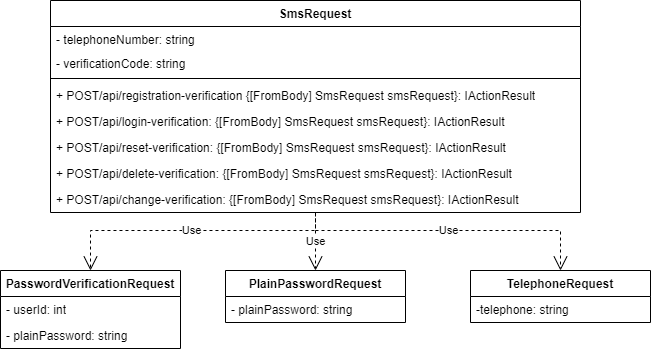
\includegraphics[scale=0.4]{SmsRequestClassDiagram.png}
	\caption{验证码请求设计UML类图设计}
\end{figure}

\begin{figure}[H]
	\centering
	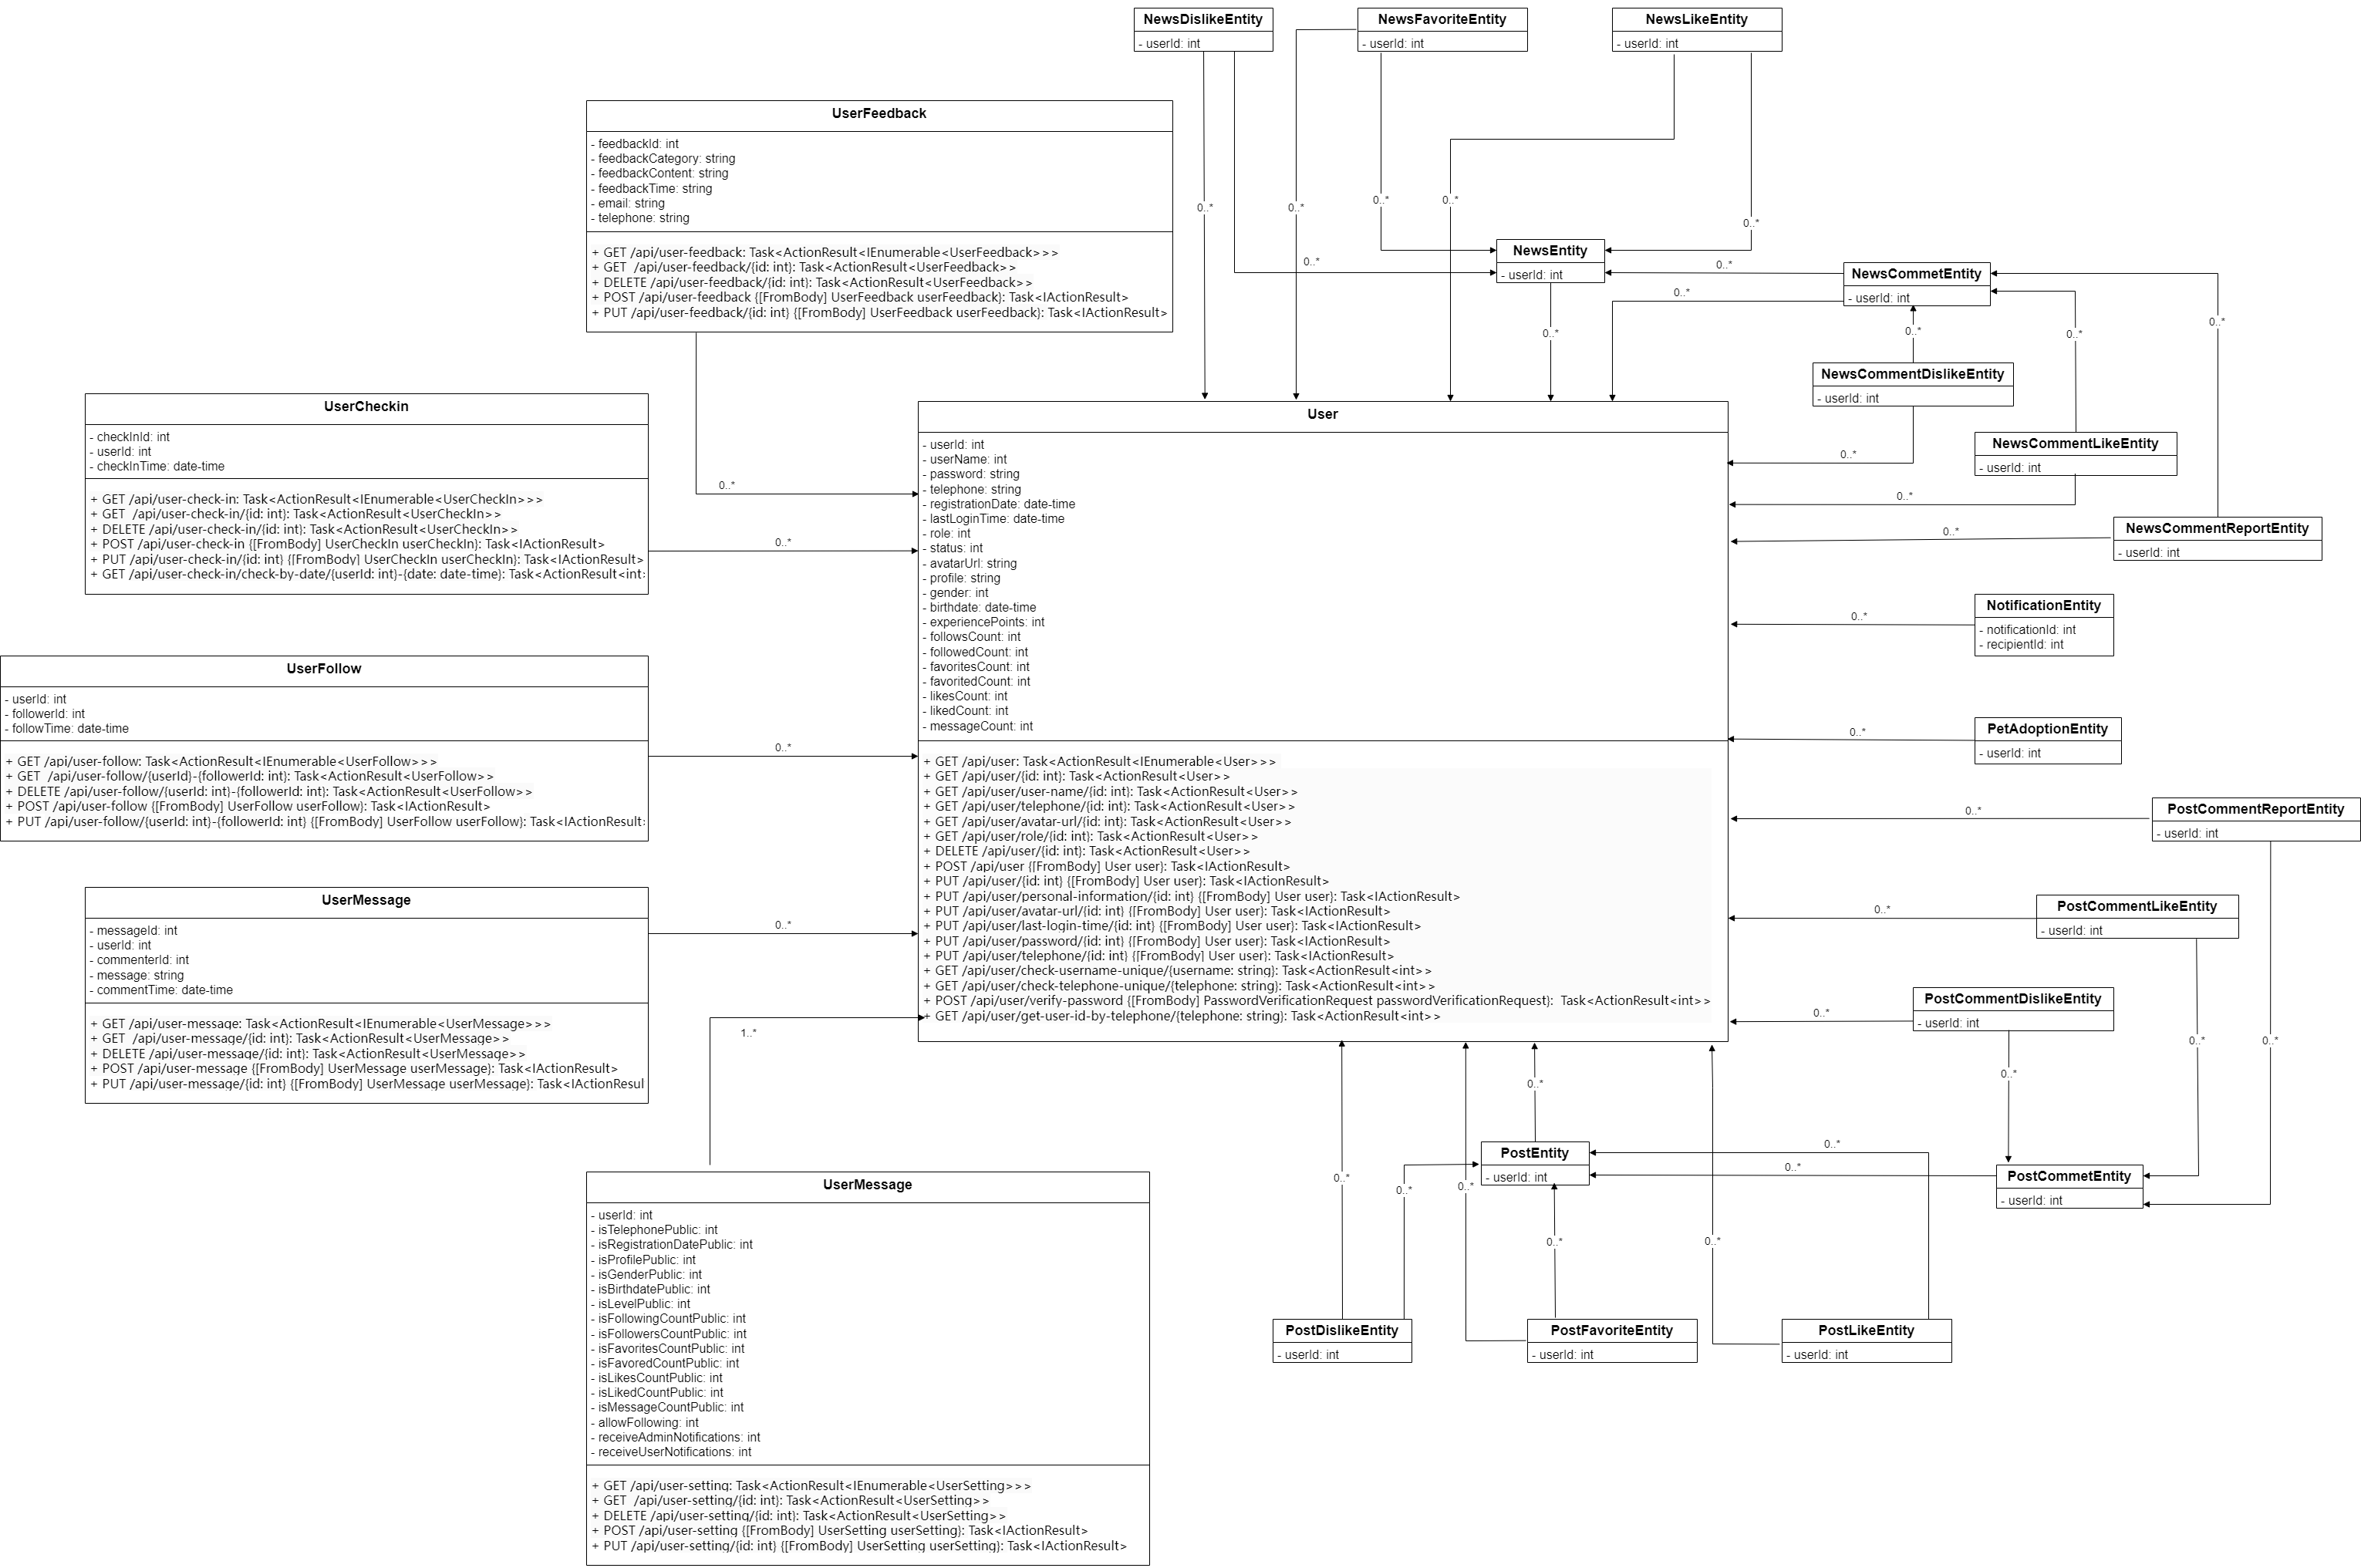
\includegraphics[scale=0.15]{UserClassDiagram.png}
	\caption{用户UML类图设计}
\end{figure}

\begin{figure}[H]
	\centering
	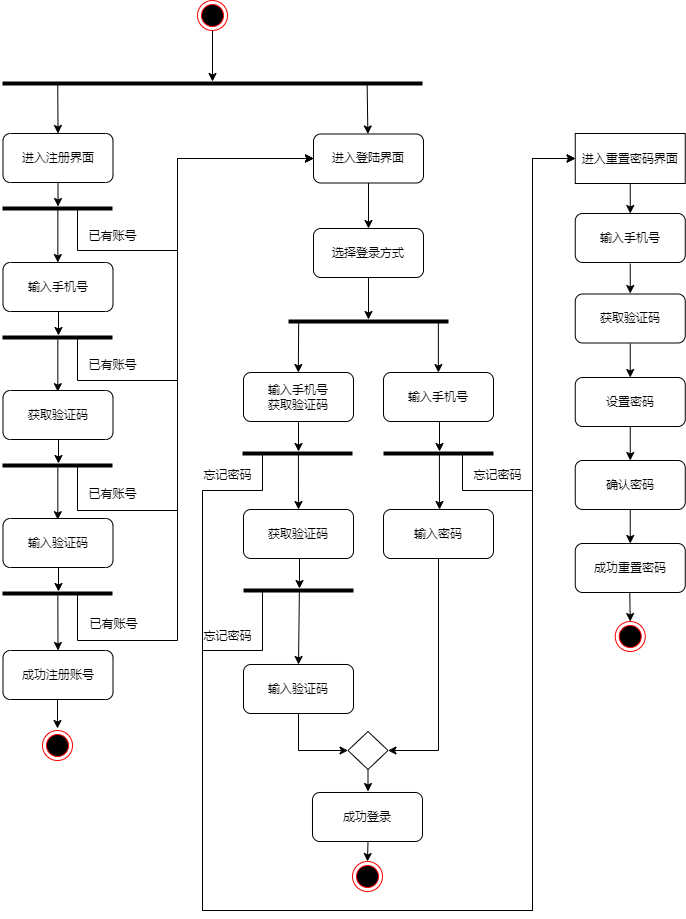
\includegraphics[scale=0.45]{AccountSystemActivityDiagram.drawio.png} 
	\caption{账号管理子系统UML活动图}
	\label{fig:AccountSystemActivityDiagram}
\end{figure}

\subsubsection{登录账号}

\begin{itemize}
	\item \textbf{界面设计}:
	\begin{figure}[H]
		\centering
		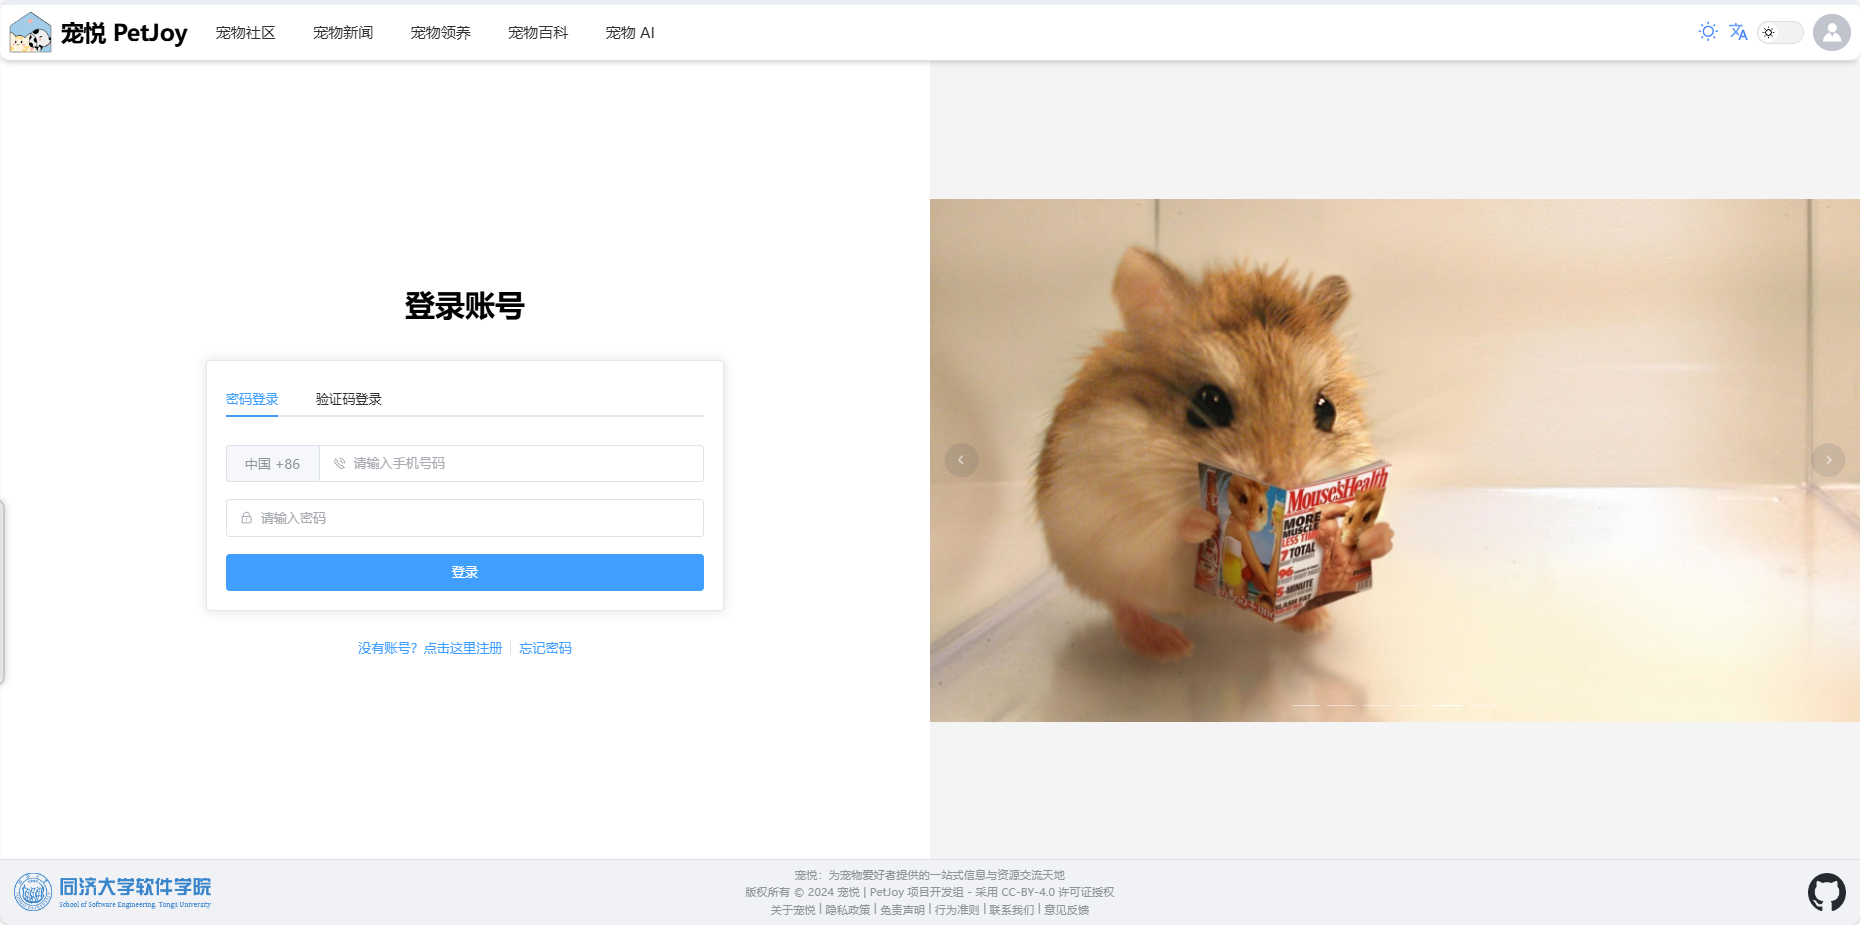
\includegraphics[scale=0.4]{Login1.png}
		\caption{登录账号}
	\end{figure}
	\item \textbf{动作序列}:
	\begin{table}[H]
		\centering
		\renewcommand\arraystretch{1.5}
		\begin{tabular}{|c|>{\raggedright\arraybackslash}p{10cm}|}
			\hline
			\textbf{动作名称} & \textbf{描述} \\ \hline
			\textbf{点击“登录”按钮} & 用户跳转到登录界面。\\ \hline
			\textbf{选择登录方式} & 用户选择密码登录或验证码登录。\\ \hline
			\textbf{输入手机号} & 用户输入自己的手机号。\\ \hline
			\textbf{输入密码或输入验证码} & 用户输入自己的密码。\\ \hline
			\textbf{点击“登录”按钮} & 用户点击登录按钮。\\ \hline
			\textbf{人类测试} & 用户完成拖拽任务。\\ \hline
		\end{tabular}
	\end{table}

	\item \textbf{用例实现}

	\textbf{点击“登录”按钮}:用户跳转到登录界面。

	\begin{figure}[H]
		\centering
		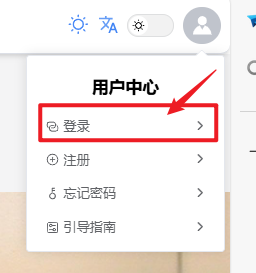
\includegraphics[scale=0.8]{Login2.png}
		\caption{用户跳转到登录界面}
	\end{figure}

	\textbf{选择登录方式}:用户选择密码登录或验证码登录。

	\begin{figure}[H]
		\centering
		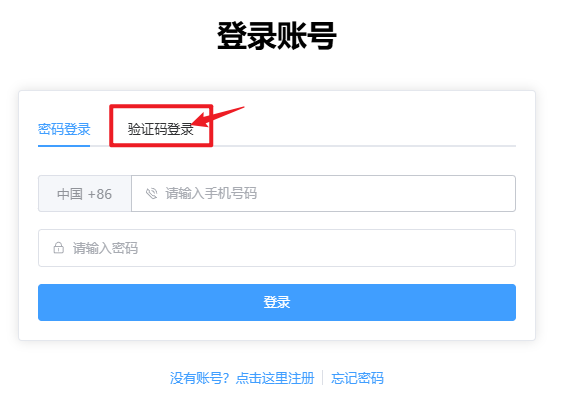
\includegraphics[scale=0.75]{Login3.png}
		\caption{选择登录方式}
	\end{figure}

	\textbf{输入手机号}:用户输入自己的手机号。

	\begin{figure}[H]
		\centering
		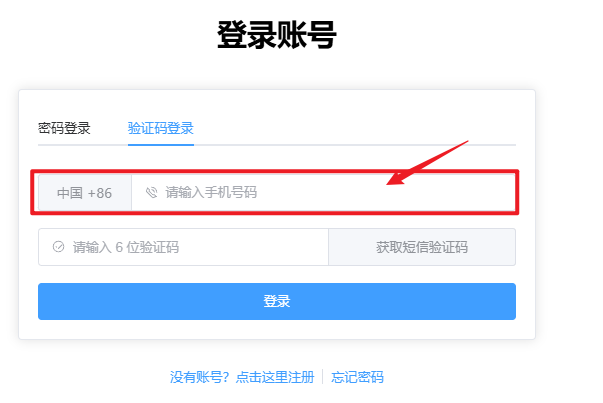
\includegraphics[scale=0.75]{Login4.png}
		\caption{输入手机号}
	\end{figure}

	\textbf{输入密码}:用户输入自己的密码。

	\begin{figure}[H]
		\centering
		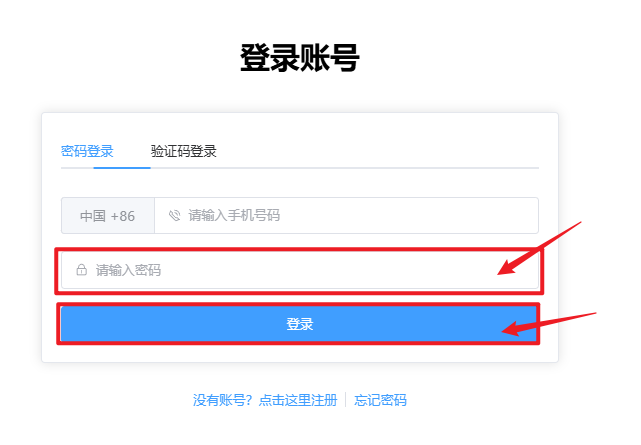
\includegraphics[scale=0.75]{Login5.png}
		\caption{输入密码}
	\end{figure}

	\textbf{输入验证码(如果使用验证码登录)}:用户输入验证码。

	\begin{figure}[H]
		\centering
		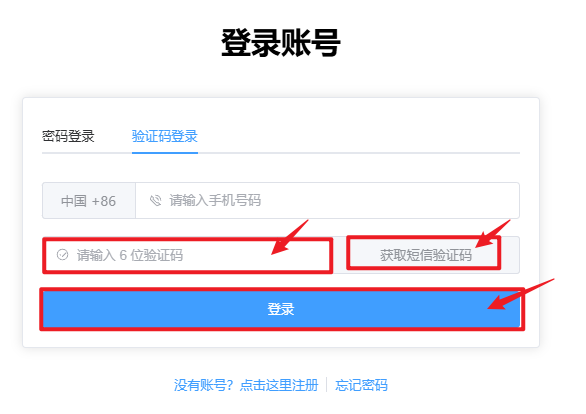
\includegraphics[scale=0.75]{Login6.png}
		\caption{输入验证码(如果使用验证码登录)}
	\end{figure}

	\textbf{人类测试}:用户完成拖拽任务。

	\begin{figure}[H]
		\centering
		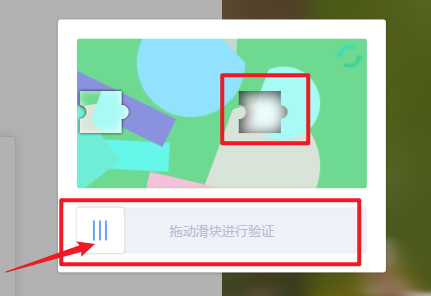
\includegraphics[scale=0.75]{Login7.png}
		\caption{人类测试}
	\end{figure}

	\item \textbf{代码实现}:
	\begin{minted}[baselinestretch=1]{html}
<template>
...
 <el-card style='width: 550px; margin-top: 16px; margin-bottom: 30px' shadow='always'>
  <el-tabs v-model='activeName'>
    <el-tab-pane :label="t('LoginPage.PasswordLogin')" name='PasswordLogin'>
      <el-form ref='loginRuleFormRef1'
               style='max-width: 100%'
               :model='loginRuleForm1'
               :rules='loginRules1'>
        <el-form-item prop='telephone'>
          <!--suppress TypeScriptValidateTypes-->
          <el-input size='large'
                    style='padding-top: 16px'
                    :placeholder="t('RegisterPage.InputTelephonePrompt')"
                    :prefix-icon='Phone'
                    v-model='loginRuleForm1.telephone'
                    clearable>
            <template #prepend>{{ t('LoginPage.TelephonePrepend') }}</template>
          </el-input>
        </el-form-item>
        <el-form-item prop='password'>
          <!--suppress TypeScriptValidateTypes-->
          <el-input v-model='loginRuleForm1.password'
                    type='password'
                    size='large'
                    :prefix-icon='Lock'
                    :placeholder="t('RegisterPage.InputPasswordPrompt')"
                    autocomplete='off'
                    show-password/>
        </el-form-item>
        <el-button type='primary'
                   size='large'
                   @click='submitLogin1(loginRuleFormRef1)'
                   style='width: 100%'>{{ t('LoginPage.Login') }}
        </el-button>
      </el-form>
    </el-tab-pane>
	
    <el-tab-pane :label="t('LoginPage.VerificationCodeLogin')" name='VerificationCodeLogin'>
      <el-form ref='loginRuleFormRef2'
               style='max-width: 100%'
               :model='loginRuleForm2'
               :rules='loginRules2'>
        <el-form-item prop='telephone'>
          <!--suppress TypeScriptValidateTypes-->
          <el-input size='large'
                    style='padding-top: 16px'
                    :placeholder="t('RegisterPage.InputTelephonePrompt')"
                    v-model='loginRuleForm2.telephone'
                    :prefix-icon='Phone'
                    clearable>
            <template #prepend>{{ t('LoginPage.TelephonePrepend') }}</template>
          </el-input>
        </el-form-item>
        <el-form-item prop='loginVerificationCode'>
          <!--suppress TypeScriptValidateTypes-->
          <el-input size='large'
                    :prefix-icon='CircleCheck'                    
                    :placeholder=
                    "t('RegisterPage.InputRegistrationVerificationCodePrompt')"
                    v-model='loginRuleForm2.loginVerificationCode'
                    clearable>
            <template #append>
              <el-button size='large'
                         type='info'
                         style='width: 200px'
                         @click='sendLoginVerificationCode'
                         :disabled='countdown>0'
                         plain>{{ buttonLabel }}
              </el-button>
            </template>
          </el-input>
        </el-form-item>
        <el-button type='primary'
                   size='large'
                   @click='submitLogin2(loginRuleFormRef2)'
                   style='width: 100%'>{{ t('LoginPage.Login') }}
        </el-button>
      </el-form>
    </el-tab-pane>
  </el-tabs>
 </el-card>
...
</template>
	\end{minted}
	
	\begin{minted}[baselinestretch=1]{typescript}
<script setup lang='ts'>
const submitLogin1 = async (formEl: FormInstance | undefined) => {
if (loginRuleForm1.password && loginRuleForm1.telephone) {
	isShowVCode.value = true
}
while (isShowVCode.value) {
	await new Promise(resolve => setTimeout(resolve, 100))
}
if (!formEl) {
	return
}
try {
	const valid = await formEl.validate();
	if (valid) {
		let userId = 0
		let isPasswordCorrect = -1
		try {
			const response = await
			axiosInstance.get(`user/get-user-id-by-telephone
			/${loginRuleForm1.telephone}`)
			userId = response.data
			try {
				const response = await axiosInstance.post
				('user/verify-password', {
					userId: userId,
					plainPassword: 
					loginRuleForm1.password
				})
				isPasswordCorrect = response.data
				if (isPasswordCorrect == -1) {
					ElMessage.error(t('LoginPage.NetworkError'))
				} else if (isPasswordCorrect == 0) {
					ElMessage.error(t('LoginPage.IncorrectPassword'))
				} else {
				try {
					axiosInstance.put(`user/last-login-time/${userId}`, {
						lastLoginTime: new Date().toISOString()
					}).then(() => {
						localStorage.setItem('currentUserId', userId.toString())
						router.push('/')
						window.location.href = '/'
					}).catch(() => {
						ElMessage.error(t('LoginPage.LoginErrorPrompt'))
					})
				} catch (error) {
					ElMessage.error(t('LoginPage.LoginErrorPrompt'))
				}
				}
			} catch (error) {
				ElMessage.error(t('LoginPage.LoginErrorPrompt'))
			}
		} catch (error) {
			ElMessage.error(t('LoginPage.LoginErrorPrompt'))
		}
	}
} catch (error) {
}
}

 async function sendLoginVerificationCode() {
    	if (countdown.value > 0) {
    		return
    	}
    	const phoneRegex = /^\d{11}$/
    	const telephone = loginRuleForm2.telephone
    	let loginVerificationCode = ''
    	for (let i = 0; i < 6; i++) {
    		loginVerificationCode += Math.floor(Math.random() * 10).toString()
    	}
    	currentCode.value = loginVerificationCode
    	currentPhone.value = loginRuleForm2.telephone
    	if (telephone != '' && phoneRegex.test(telephone) 
    	&& isTelephoneUnique.value == 0) {
    		ElMessage.warning(t('LoginPage.NotRegistered'))
    	}
    	if (telephone != '' && phoneRegex.test(telephone) 
    	&& isTelephoneUnique.value == 1) {
    		console.log('Telephone: ' + 
    		(currentPhone.value == '' ? 'null' : currentPhone.value)
    		 + ' - Code: ' + currentCode.value)
    		countdown.value = 60
    		const intervalId = setInterval(() => {
    			countdown.value--
    			if (countdown.value <= 0) {
    				clearInterval(intervalId)
    			}
    		}, 1000)
    		const body = {telephoneNumber: telephone, verificationCode:
    			 loginVerificationCode}
    		try {
    			await axiosInstance.post('login-verification', body)
    		} catch (error) {
    			ElNotification({
    				title: 
    				t('RegisterPage.VerificationCodeSendingFailed'),
    				message: 
    				t('RegisterPage.VerificationCodeSendingFailedPrompt'),
    				type: 'error',
    			})
    		}
    	}
 }
 
 const submitLogin2 = async (formEl: FormInstance | undefined) => {
    	if (loginRuleForm2.loginVerificationCode && loginRuleForm2.telephone) {
    		isShowVCode.value = true
    	}
    	while (isShowVCode.value) {
    		await new Promise(resolve => setTimeout(resolve, 100))
    	}
    	if (!formEl) {
    		return
    	}
    	try {
    		const valid = await formEl.validate();
    		if (valid) {
    			let userId = 0
    			try {
    				const response = await axiosInstance.get
    				(`user/get-user-id-by-telephone/${loginRuleForm2.telephone}`)
    				userId = response.data
    				localStorage.setItem('currentUserId', userId.toString())
    				await router.push('/')
    				window.location.href = '/'
    			} catch (error) {
    				ElMessage.error(t('LoginPage.LoginErrorPrompt'))
    			}
    		}
    	} catch (error) {
    	}
 }

</script>
	\end{minted}

\end{itemize}

\subsubsection{注册账号}

\begin{itemize}
\item \textbf{界面设计}:
	\begin{figure}[H]
		\centering
		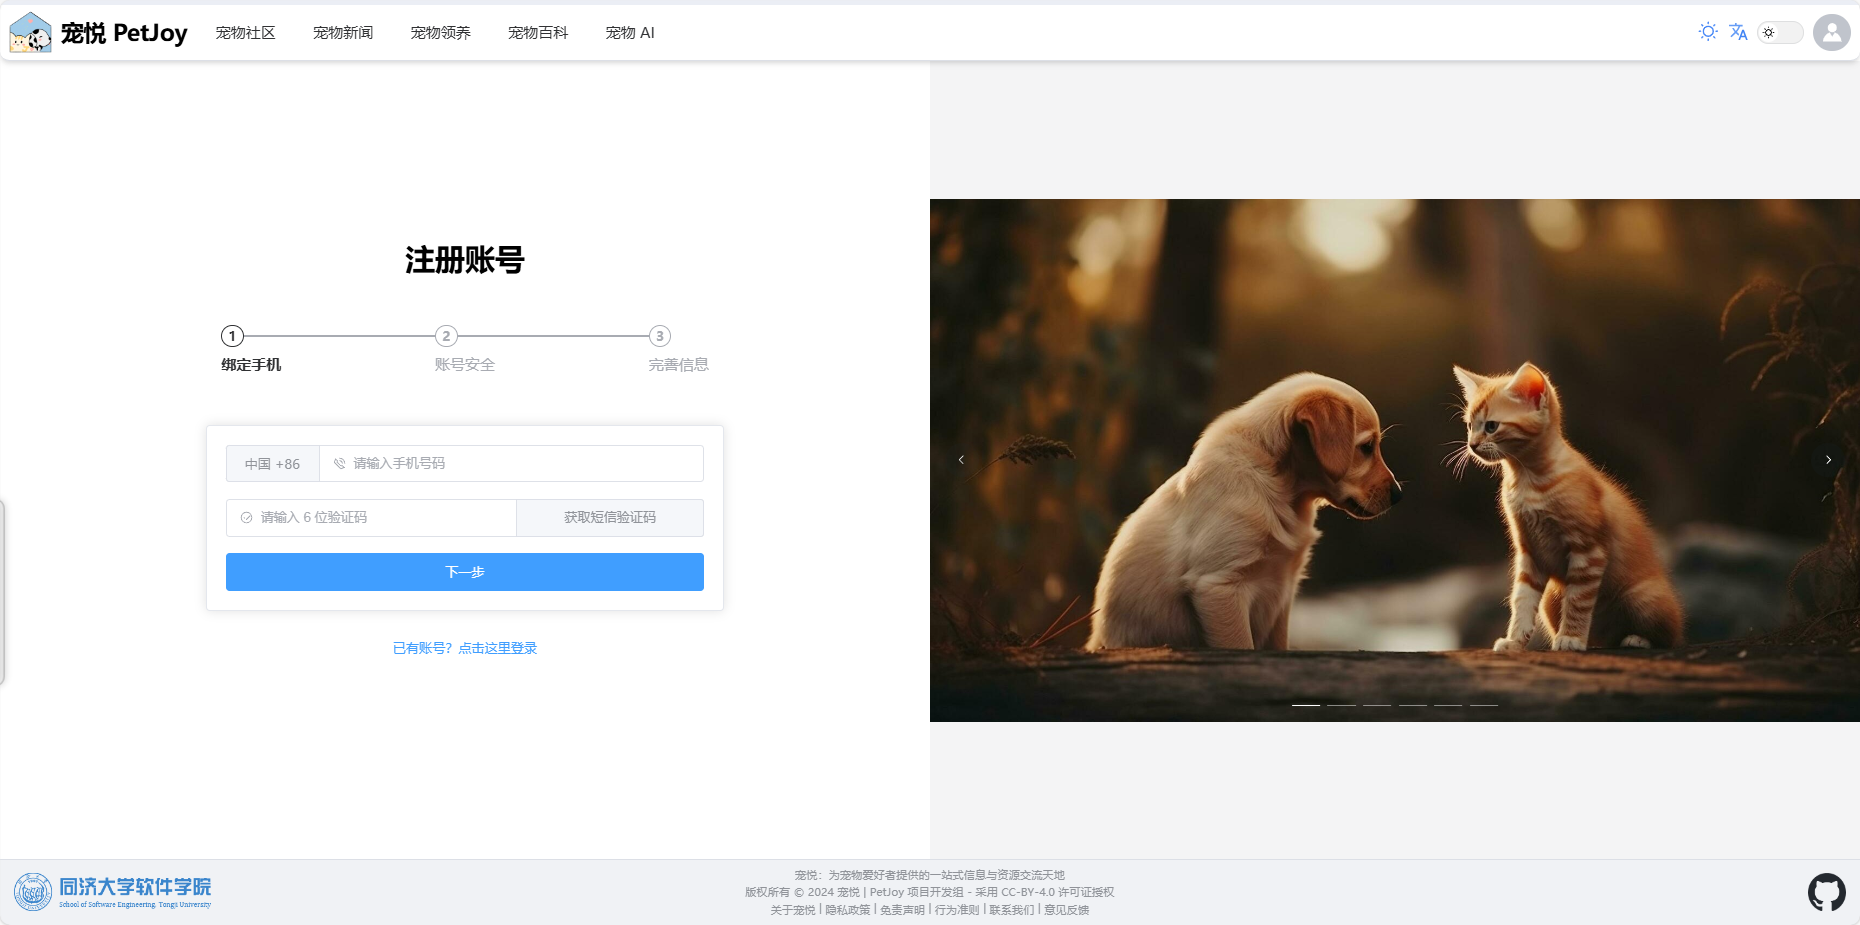
\includegraphics[scale=0.4]{Register1.png}
		\caption{注册账号}
	\end{figure}
	\item \textbf{动作序列}:
	\begin{table}[H]
		\centering
		\renewcommand\arraystretch{1.5}
		\begin{tabular}{|c|>{\raggedright\arraybackslash}p{10cm}|}
			\hline
			\textbf{动作名称} & \textbf{描述} \\ \hline
			\textbf{点击“注册”按钮} & 用户可以跳转到注册界面。\\ \hline
			\textbf{输入手机号} & 用户可以将新账号与一个未注册过的手机号绑定。\\ \hline
			\textbf{点击“获取验证码”按钮} & 用户可以通过输入的手机号获取验证码并输入到验证框内。\\ \hline
			\textbf{点击“下一步”按钮} & 用户可以进入到密码设置页面。\\ \hline
			\textbf{输入个性化密码} & 用户可以根据系统提示输入合法密码并确认。\\ \hline
			\textbf{点击“下一步”按钮} & 用户可以进入到信息完善页面。\\ \hline
			\textbf{输入昵称、点击选项按钮} & 用户可根据自己的个人信息完善平台的账户信息。\\ \hline
		\end{tabular}
	\end{table}

	\item \textbf{用例实现}

	\textbf{点击“注册”按钮}:用户可以跳转到注册界面。

	\begin{figure}[H]
		\centering
		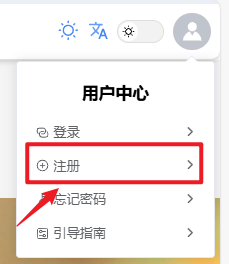
\includegraphics[scale=0.8]{Register2.png}
		\caption{用户可以跳转到注册界面}
	\end{figure}

	\textbf{输入手机号}:用户可以将新账号与一个未注册过的手机号绑定。

	\begin{figure}[H]
		\centering
		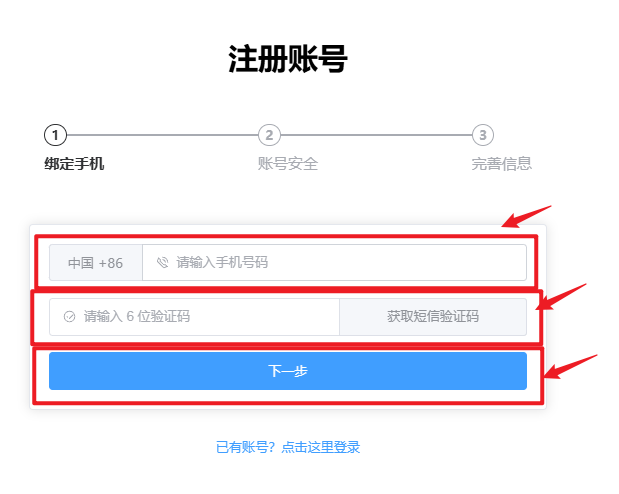
\includegraphics[scale=0.75]{Register3.png}
		\caption{输入手机号}
	\end{figure}

	\textbf{输入个性化密码}:用户可以根据系统提示输入合法密码并确认。

	\begin{figure}[H]
		\centering
		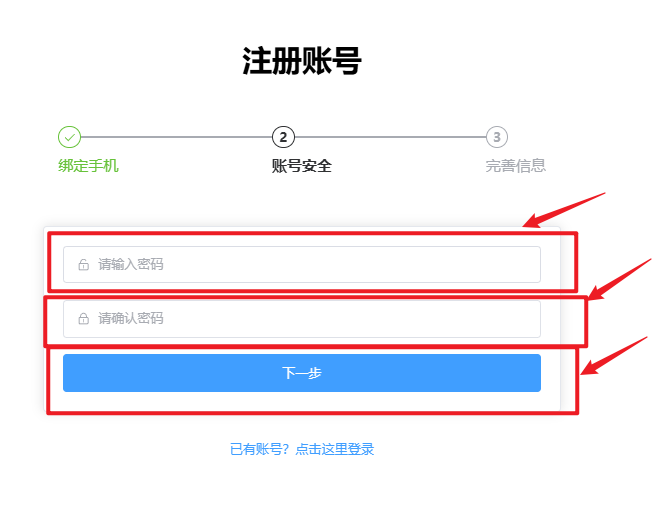
\includegraphics[scale=0.75]{Register4.png}
		\caption{输入个性化密码}
	\end{figure}

	\textbf{输入昵称、点击选项按钮}:用户可根据自己的个人信息完善平台的账户信息。

	\begin{figure}[H]
		\centering
		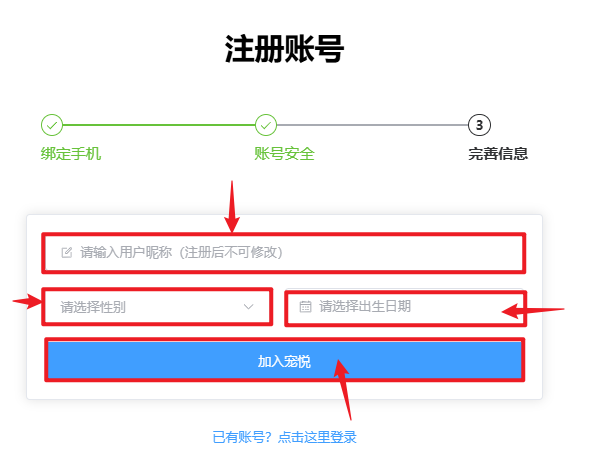
\includegraphics[scale=0.75]{Register5.png}
		\caption{输入昵称、点击选项按钮}
	\end{figure}

	\item \textbf{代码实现}:
	\begin{minted}[baselinestretch=1]{html}
<template>
...
 <div class='left'>
  <h1 style='margin-bottom: 50px'>{{ t('RegisterPage.RegisterAccount') }}</h1>
	
  <el-steps style='width: 520px' :active='activeStep' finish-status='success'>
    <el-step :title="t('RegisterPage.BindPhone')"/>
    <el-step :title="t('RegisterPage.AccountSecurity')"/>
    <el-step :title="t('RegisterPage.CompleteInformation')"/>
  </el-steps>
	
  <el-card style='width: 550px; margin-top: 50px; margin-bottom: 30px' shadow='always'>
    <div v-if='activeStep==0'>
      <el-form ref='registrationRuleFormRef1'
               style='max-width: 100%'
               :model='registrationRuleForm1'
               :rules='registrationRules'>
        <el-form-item prop='telephone'>
          <!--suppress TypeScriptValidateTypes-->
          <el-input size='large'
                    :placeholder="t('RegisterPage.InputTelephonePrompt')"
                    v-model='registrationRuleForm1.telephone'
                    :prefix-icon='Phone'
                    clearable>
            <template #prepend>{{ t('LoginPage.TelephonePrepend') }}</template>
          </el-input>
        </el-form-item>
        <el-form-item prop='registrationVerificationCode'>
          <!--suppress TypeScriptValidateTypes-->
          <el-input size='large'
                    :placeholder="t('RegisterPage.InputRegistrationVerificationCodePrompt')"
                    v-model='registrationRuleForm1.registrationVerificationCode'
                    :prefix-icon='CircleCheck'
                    clearable>
            <template #append>
              <el-button size='large'
                         type='info'
                         style='width: 200px'
                         @click='sendRegistrationVerificationCode'
                         :disabled='countdown>0'
                         plain>
                {{ buttonLabel }}
              </el-button>
            </template>
          </el-input>
        </el-form-item>
        <el-button type='primary'
                   size='large'
                   @click='submitRegistration(registrationRuleFormRef1)'
                   style='width: 100%'>{{ t('RegisterPage.NextStep') }}
        </el-button>
      </el-form>
    </div>
  ...同上,略
  </el-card>
	
  <el-link style='margin-bottom: 50px' type='primary' 
  :underline='false' @click="router.push('/login')">
    {{ t('RegisterPage.HaveAnAccountPrompt') }}
  </el-link>
 </div>
...
</template>
	\end{minted}
	
	\begin{minted}[baselinestretch=1]{typescript}
	<script setup lang='ts'>
	
	</script>
	\end{minted}

\end{itemize}

\subsubsection{登出账号}

\begin{itemize}
	\item \textbf{界面设计}:
	\begin{figure}[H]
		\centering
		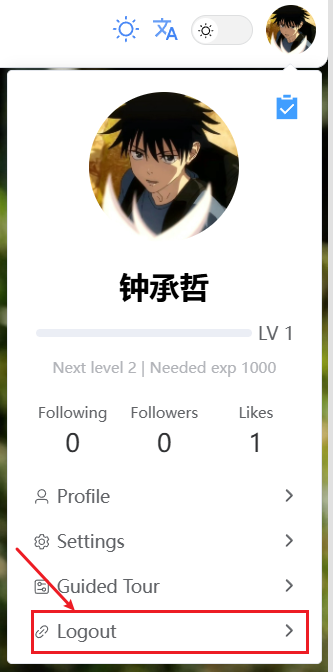
\includegraphics[scale=0.8]{Logout.png}
		\caption{登出账号}
	\end{figure}
	\item \textbf{动作序列}:
	\begin{table}[H]
		\centering
		\renewcommand\arraystretch{1.5}
		\begin{tabular}{|c|>{\raggedright\arraybackslash}p{10cm}|}
			\hline
			\textbf{动作名称} & \textbf{描述} \\ \hline
			\textbf{点击“退出登录”按钮} & 用户可以安全地退出登录状态。\\ \hline
		\end{tabular}
	\end{table}
	
	\item \textbf{用例实现}

	\textbf{点击“退出登录”按钮}:用户可以安全地退出登录状态。

	\begin{figure}[H]
		\centering
		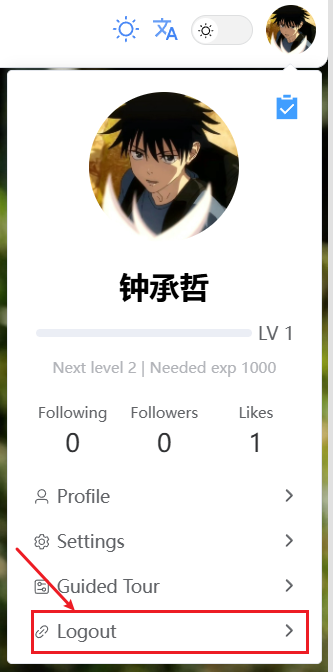
\includegraphics[scale=0.8]{Logout.png}
		\caption{用户可以安全地退出登录状态}
	\end{figure}

	\item \textbf{代码实现}:
	\begin{minted}[baselinestretch=1]{html}
	<template>
	...
 <el-dropdown-item :icon='Link' @click='logout'>
  <div class='dropdown-item'>
    <span>{{ t('HeaderNavbar.Logout') }}</span>
    <span><el-icon :size='12' class='dropdown-item-icon'>
    <ArrowRightBold/></el-icon></span>
  </div>
 </el-dropdown-item>
	...
	</template>
	\end{minted}
	
    \begin{minted}[baselinestretch=1]{typescript}
<script setup lang='ts'>
function logout() {
  	localStorage.setItem('currentUserId', '0')
  	router.push('/')
  	window.location.href = '/'
}
</script>
    \end{minted}
\end{itemize}

\subsubsection{账号安全性保护}

\paragraph{重置密码}

\begin{itemize}
\item \textbf{界面设计}:
	\begin{figure}[H]
		\centering
		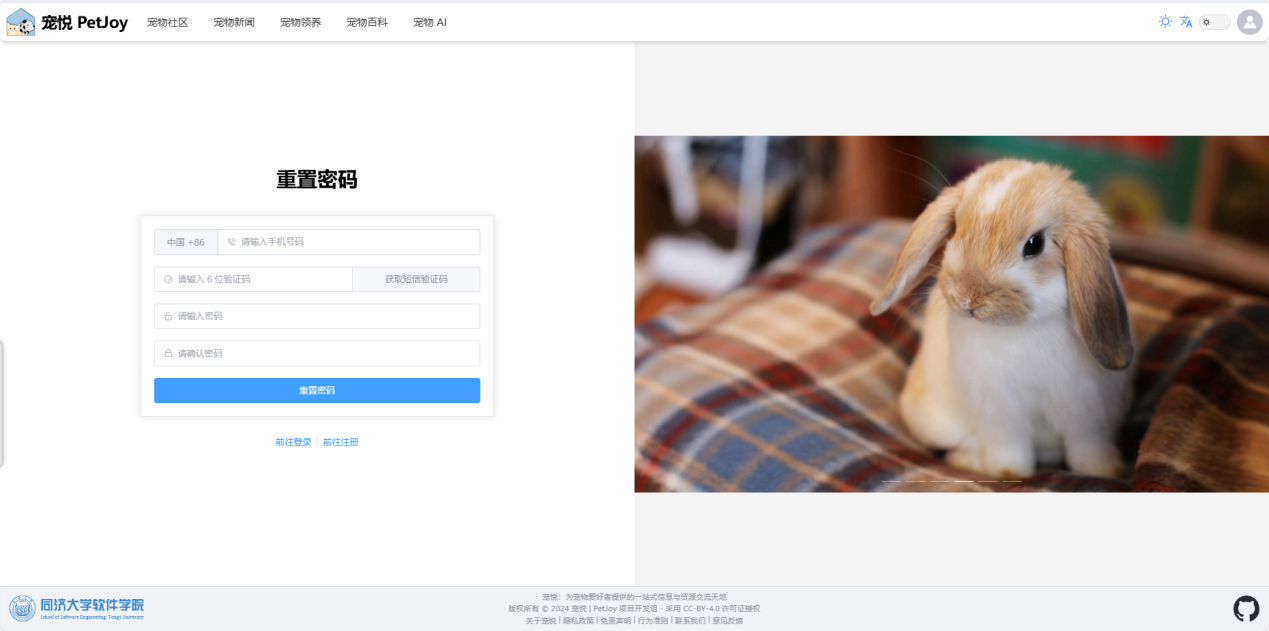
\includegraphics[scale=0.8]{ResetPassword1.png}
		\caption{重置密码}
	\end{figure}
	\item \textbf{动作序列}:
	\begin{table}[H]
		\centering
		\renewcommand\arraystretch{1.5}
		\begin{tabular}{|c|>{\raggedright\arraybackslash}p{10cm}|}
			\hline
			\textbf{动作名称} & \textbf{描述} \\ \hline
			\textbf{点击“忘记密码”或者“重置密码”按钮} & 用户跳转到重置密码页面。\\ \hline
			\textbf{输入手机号} & 用户输入自己账号绑定的手机号进行密码重置。\\ \hline
			\textbf{输入新密码} & 用户输入自己的新密码并二次确认新密码。\\ \hline
			\textbf{点击“重置密码”按钮} & 用户重置密码成功。\\ \hline
		\end{tabular}
	\end{table}

	\item \textbf{用例实现}

	\textbf{点击“忘记密码”或者“重置密码”按钮}:用户跳转到重置密码页面。

	\begin{figure}[H]
		\centering
		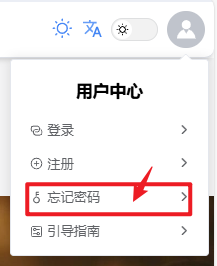
\includegraphics[scale=0.8]{ResetPassword2.png}
		\caption{用户跳转到重置密码页面}
	\end{figure}

	\textbf{输入手机号}:用户输入自己账号绑定的手机号进行密码重置。

	\begin{figure}[H]
		\centering
		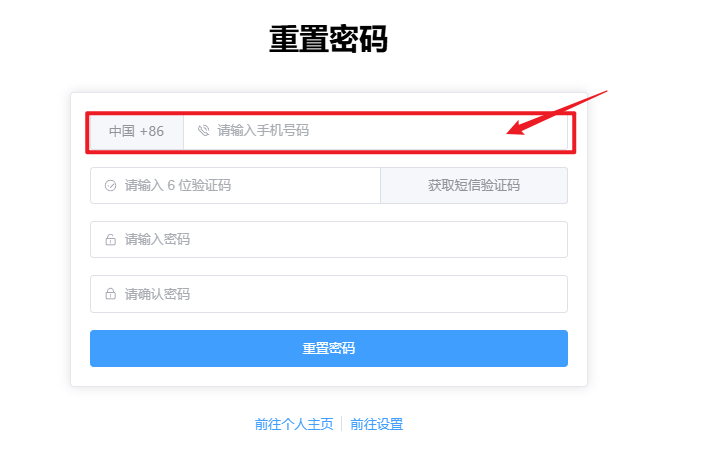
\includegraphics[scale=0.8]{ResetPassword3.png}
		\caption{输入手机号}
	\end{figure}

	\textbf{输入新密码}:用户输入自己的新密码并二次确认新密码。

	\begin{figure}[H]
		\centering
		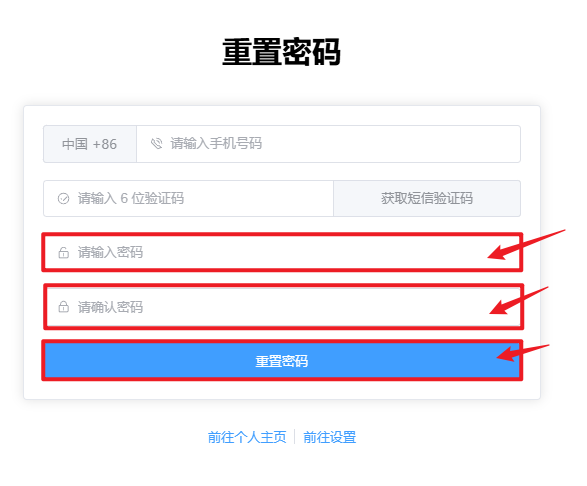
\includegraphics[scale=0.8]{ResetPassword4.png}
		\caption{输入新密码}
	\end{figure}

	\item \textbf{代码实现}:
	\begin{minted}[baselinestretch=1]{html}
<template>
...
 <div class='left'>
  <h1>{{ t('ResetPasswordPage.ResetPassword') }}</h1>
	
  <el-card style='width: 550px; margin-top: 16px; margin-bottom: 30px' shadow='always'>
    <el-form ref='resetPasswordRuleFormRef'
             style='max-width: 100%'
             :model='resetPasswordRuleForm'
             :rules='resetPasswordRules'>
      <el-form-item prop='telephone'>
        <!--suppress TypeScriptValidateTypes-->
        <el-input size='large'
                  :placeholder="t('RegisterPage.InputTelephonePrompt')"
                  v-model='resetPasswordRuleForm.telephone'
                  :prefix-icon='Phone'
                  clearable>
          <template #prepend>{{ t('LoginPage.TelephonePrepend') }}</template>
        </el-input>
      </el-form-item>
      ...同上,略
      <el-button type='primary'
                 size='large'
                 @click='submitResetPassword(resetPasswordRuleFormRef)'
                 style='width: 100%'>{{ t('ResetPasswordPage.ResetPassword') }}
      </el-button>
    </el-form>
  </el-card>
	
  <div v-if='currentUserId==0' style='display: flex; padding-bottom: 46px'>
    <el-link type='primary' :underline='false' @click="router.push('/login')">
      {{ t('ResetPasswordPage.GoToLogin') }}
    </el-link>
    <el-divider direction='vertical' style='margin-top: 1px'/>
    <el-link type='primary' :underline='false' @click="router.push('/register')">
      {{ t('ResetPasswordPage.GoToRegister') }}
    </el-link>
  </div>
	
  <div v-if='currentUserId!=0' style='display: flex; padding-bottom: 46px'>
    <el-link type='primary' :underline='false' 
    @click="router.push(`/profile/${currentUserId}`)">
      {{ t('ResetPasswordPage.GoToProfile') }}
    </el-link>
    <el-divider direction='vertical' style='margin-top: 1px'/>
    <el-link type='primary' :underline='false' @click="router.push('/settings')">
      {{ t('ResetPasswordPage.GoToSettings') }}
    </el-link>
  </div>
 </div>
...
</template>
	\end{minted}
	
	\begin{minted}[baselinestretch=1]{typescript}
<script setup lang='ts'>
...
	const router = useRouter()
	...
	const submitResetPassword = async (formEl: FormInstance | undefined) => {
		if (resetPasswordRuleForm.resetVerificationCode
		&& resetPasswordRuleForm.telephone
		&& resetPasswordRuleForm.password
		&& resetPasswordRuleForm.passwordCheck) {
			isShowVCode.value = true
		}
		while (isShowVCode.value) {
			await new Promise(resolve => setTimeout(resolve, 100))
		}
		if (!formEl) {
			return
		}
		try {
		const valid = await formEl.validate();
		if (valid) {
		try {
			await axiosInstance.get(`user/get-user-id-by-telephone/
			${resetPasswordRuleForm.telephone}`).then((response) => {
				axiosInstance.put(`user/password/${response.data}`, 
				{plainPassword: resetPasswordRuleForm.password}).then(() => {
					localStorage.setItem('currentUserId', '0')
					router.push('/login')
					window.location.href = '/login'
				}).catch(() => {
				ElMessage.error(t('ResetPasswordPage.ResetPasswordErrorPrompt'))
				})
			}).catch(() => {
				ElMessage.error(t('ResetPasswordPage.ResetPasswordErrorPrompt'))
			})
		} catch (error) {
			ElMessage.error(t('ResetPasswordPage.ResetPasswordErrorPrompt'))
		}
		}
		} catch (error) {
		}
	}
	...
</script>
	\end{minted}

\end{itemize}

\paragraph{修改绑定手机号}

\begin{itemize}
\item \textbf{界面设计}:
	\begin{figure}[H]
		\centering
		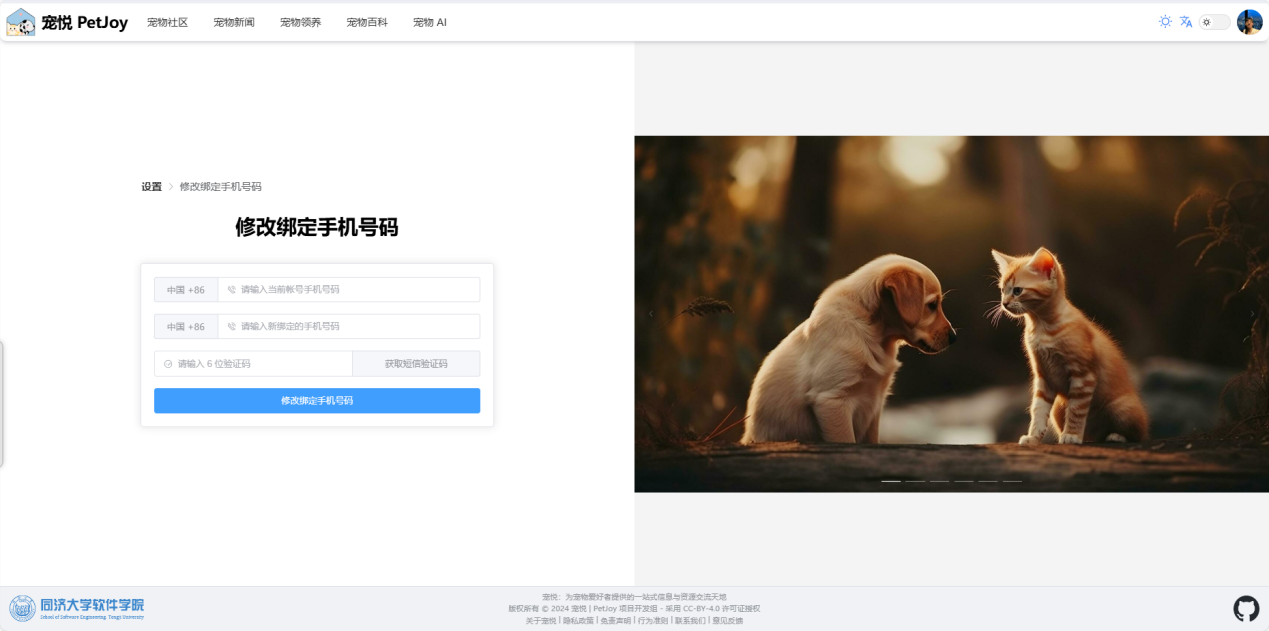
\includegraphics[scale=0.8]{ResetNumber1.png}
		\caption{修改绑定手机号}
	\end{figure}
	\item \textbf{动作序列}:
	\begin{table}[H]
		\centering
		\renewcommand\arraystretch{1.5}
		\begin{tabular}{|c|>{\raggedright\arraybackslash}p{10cm}|}
			\hline
			\textbf{动作名称} & \textbf{描述} \\ \hline
			\textbf{点击“修改绑定手机号”按钮} & 用户跳转到修改绑定手机号页面。\\ \hline
			\textbf{用户输入旧的手机号和新的手机号} & 用户分别输入新旧手机号进行重新绑定。\\ \hline
			\textbf{点击“获取验证码”按钮} & 用户获取验证码进行新的手机号验证。\\ \hline
		\end{tabular}
	\end{table}

	\item \textbf{用例实现}

	\textbf{点击“修改绑定手机号”按钮}:用户跳转到修改绑定手机号页面。

	\begin{figure}[H]
		\centering
		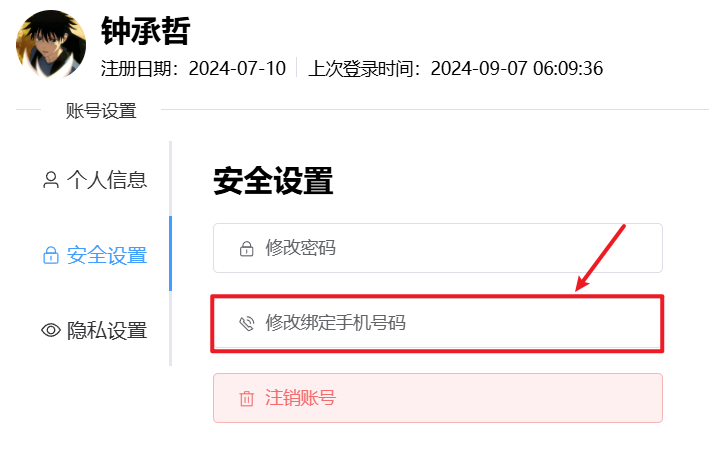
\includegraphics[scale=0.8]{ResetNumber2.png}
		\caption{用户跳转到修改绑定手机号页面}
	\end{figure}

	\textbf{用户输入旧的手机号和新的手机号}:用户分别输入新旧手机号进行重新绑定。

	\begin{figure}[H]
		\centering
		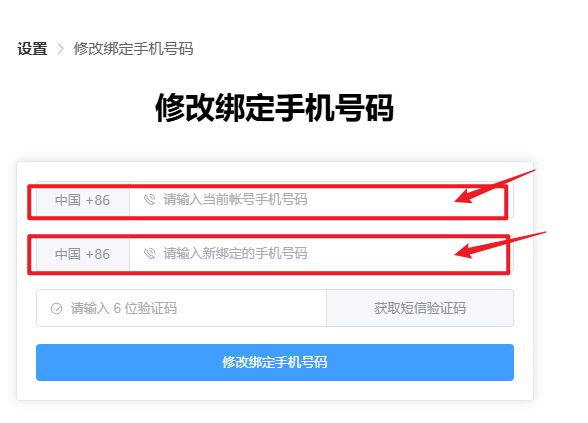
\includegraphics[scale=0.8]{ResetNumber3.png}
		\caption{用户输入旧的手机号和新的手机号}
	\end{figure}

	\textbf{点击“获取验证码”按钮}:用户获取验证码进行新的手机号验证。

	\begin{figure}[H]
		\centering
		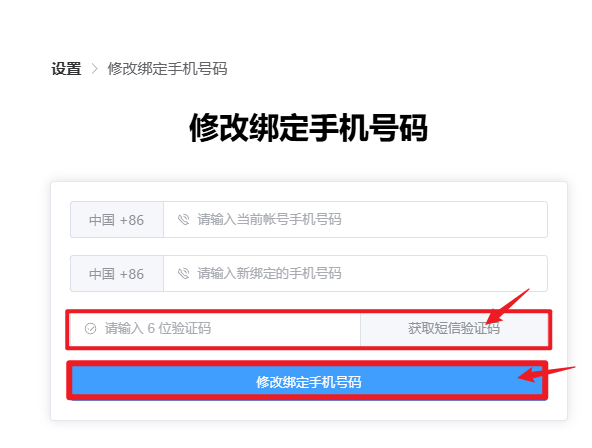
\includegraphics[scale=0.8]{ResetNumber4.png}
		\caption{用户获取验证码进行新的手机号验证}
	\end{figure}

	\item \textbf{代码实现}:
	\begin{minted}[baselinestretch=1]{html}
<template>
...
 <div class='container'>
  <div class='left'>
    <div style='width: 550px'>
      <!--suppress TypeScriptValidateTypes-->
      <el-breadcrumb :separator-icon='ArrowRight' class='breadcrumb-with-margin'>
        <el-breadcrumb-item to='/settings'>{{ t('HeaderNavbar.Settings') }}</el-breadcrumb-item>
        <el-breadcrumb-item>{{ t('SettingsPage.ChangeBoundTelephone') }}</el-breadcrumb-item>
      </el-breadcrumb>
    </div>
	
    <h1>{{ t('SettingsPage.ChangeBoundTelephone') }}</h1>
	
    <el-card style='width: 550px; margin-top: 16px; margin-bottom: 30px' shadow='always'>
      <el-form ref='changeTelephoneRuleFormRef'
               style='max-width: 100%'
               :model='changeTelephoneRuleForm'
               :rules='changeTelephoneRules'>
        <el-form-item prop='currentTelephone'>
          <!--suppress TypeScriptValidateTypes-->
          <el-input size='large'
                    :placeholder="t('ChangeTelephonePage.InputCurrentTelephonePrompt')"
                    v-model='changeTelephoneRuleForm.currentTelephone'
                    :prefix-icon='Phone'
                    clearable>
            <template #prepend>{{ t('LoginPage.TelephonePrepend') }}</template>
          </el-input>
        </el-form-item>
        <el-form-item prop='telephone'>
          <!--suppress TypeScriptValidateTypes-->
          <el-input size='large'
                    :placeholder="t('ChangeTelephonePage.InputBoundTelephonePrompt')"
                    v-model='changeTelephoneRuleForm.telephone'
                    :prefix-icon='Phone'
                    clearable>
          <template #prepend>{{ t('LoginPage.TelephonePrepend') }}</template>
        </el-input>
      </el-form-item>
      <el-form-item prop='changeVerificationCode'>
        <!--suppress TypeScriptValidateTypes-->
        <el-input size='large'
                  :placeholder="t('RegisterPage.InputRegistrationVerificationCodePrompt')"
                  v-model='changeTelephoneRuleForm.changeVerificationCode'
                  :prefix-icon='CircleCheck'
                  clearable>
          <template #append>
            <el-button size='large'
                       type='info'
                        style='width: 200px'
                       @click='sendChangeVerificationCode'
                       :disabled='countdown>0'
                       plain>
              {{ buttonLabel }}
            </el-button>
          </template>
        </el-input>
      </el-form-item>
      <el-button type='primary'
                 size='large'
                 @click='submitChangeTelephone(changeTelephoneRuleFormRef)'
                 style='width: 100%'>{{ t('SettingsPage.ChangeBoundTelephone') }}
      </el-button>
    </el-form>
  </el-card>
 </div>
	
 <div v-if='windowWidth>=1200' class='right'>
  <div class='carousel-container'>
    <el-carousel trigger='click' :interval='3000' motion-blur height='calc(50vw * 9 / 16)'>
      <el-carousel-item v-for='(img, index) in carouselImages' :key='index'>
        <img :src='img' alt='CarouselImages' class='carousel-image'>
      </el-carousel-item>
    </el-carousel>
  </div>
 </div>
	</div>
	
	<Vcode :show='isShowVCode'
     @success='isShowVCode=false'
     @fail='isShowVCode=true'
     @close='isShowVCode=true'
     :successText="t('RegisterPage.VerificationSuccessful')"
     :failText="t('RegisterPage.VerificationFailed')"
     :sliderText="t('RegisterPage.DragTheSliderToVerify')"/>
...
</template>
	\end{minted}
	
	\begin{minted}[baselinestretch=1]{typescript}
<script setup lang='ts'>
const submitChangeTelephone = async (formEl: FormInstance | undefined) => {
	if (changeTelephoneRuleForm.changeVerificationCode && changeTelephoneRuleForm.telephone) {
		isShowVCode.value = true
	}
	while (isShowVCode.value) {
		await new Promise(resolve => setTimeout(resolve, 100))
	}
	if (!formEl) {
		return
	}
	try {
		const valid = await formEl.validate();
		if (valid) {
			try {
				axiosInstance.put(`user/telephone/$
				{currentUserId.value}`, {
					telephone: changeTelephoneRuleForm.telephone
				}).then(() => {
					localStorage.setItem('currentUserId', '0')
					router.push('/login')
					window.location.href = '/login'
				}).catch(() => {
					ElMessage.error(t('ErrorMessage.PutErrorMessage'))
				})
			} catch (error) {
				ElMessage.error(t('ErrorMessage.PutErrorMessage'))
			}
		}
	} catch (error) {
}
}
</script>
	\end{minted}

\end{itemize}

\paragraph{注销账号}

\begin{itemize}
\item \textbf{界面设计}:
	\begin{figure}[H]
		\centering
		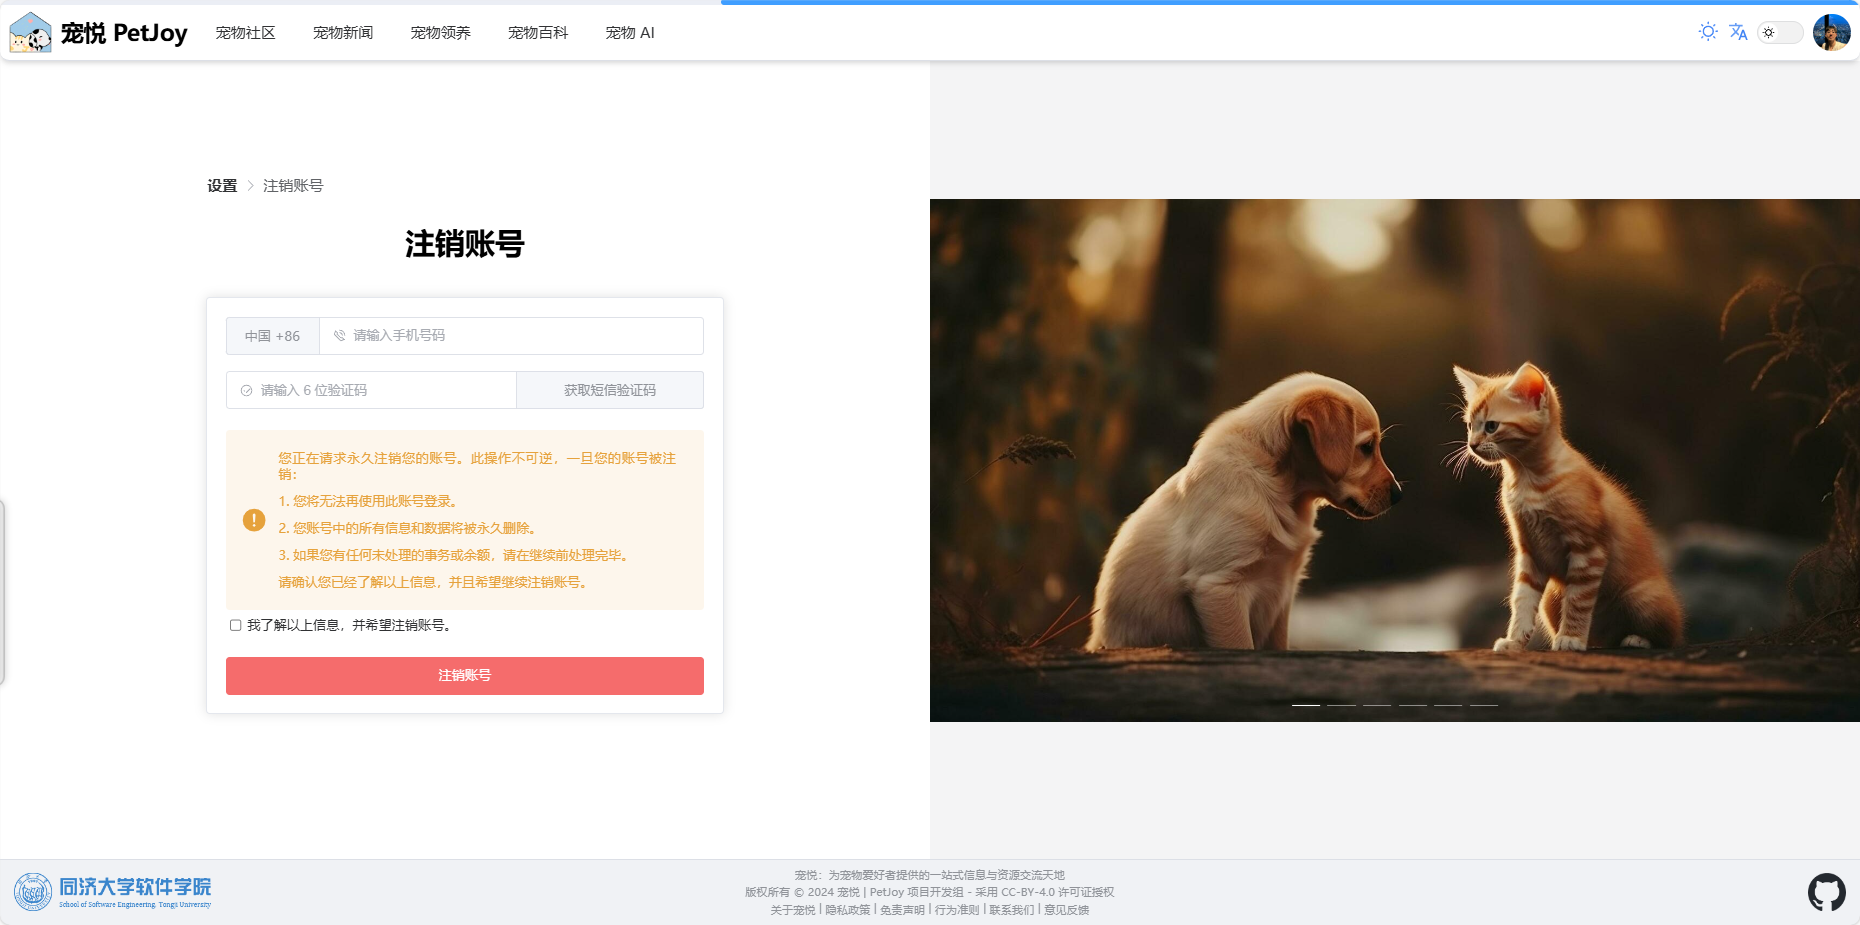
\includegraphics[scale=0.4]{DeleteAccount1.png}
		\caption{注销账号}
	\end{figure}
	\item \textbf{动作序列}:
	\begin{table}[H]
		\centering
		\renewcommand\arraystretch{1.5}
		\begin{tabular}{|c|>{\raggedright\arraybackslash}p{10cm}|}
			\hline
			\textbf{动作名称} & \textbf{描述} \\ \hline
			\textbf{点击“注销账号”按钮} & 用户跳转到注销账号页面。\\ \hline
			\textbf{用户输入密码} & 用户输入自己的手机号并通过验证码验证进行账号注销。\\ \hline
			\textbf{点击“注销账号”按钮} & 用户注销账号成功。\\ \hline
		\end{tabular}
	\end{table}

	\item \textbf{用例实现}

	\textbf{点击“注销账号”按钮}:用户跳转到注销账号页面。

	\begin{figure}[H]
		\centering
		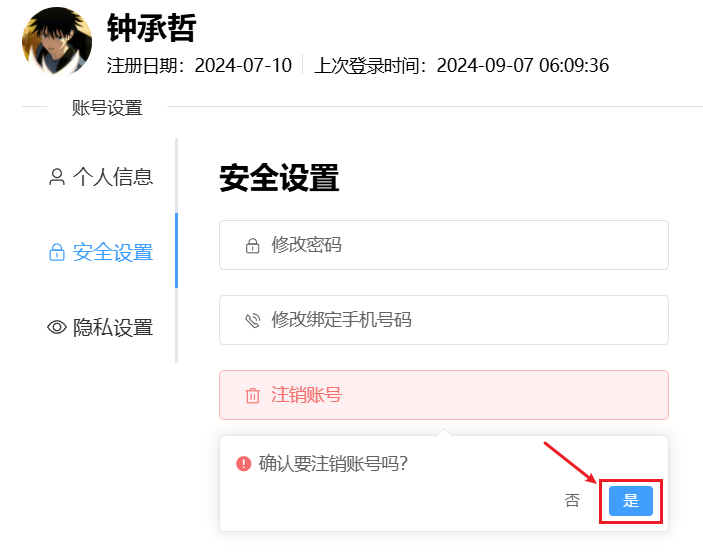
\includegraphics[scale=0.8]{DeleteAccount2.png}
		\caption{用户跳转到注销账号页面}
	\end{figure}

	\textbf{用户输入密码}:用户输入自己的手机号并通过验证码验证进行账号注销。

	\begin{figure}[H]
		\centering
		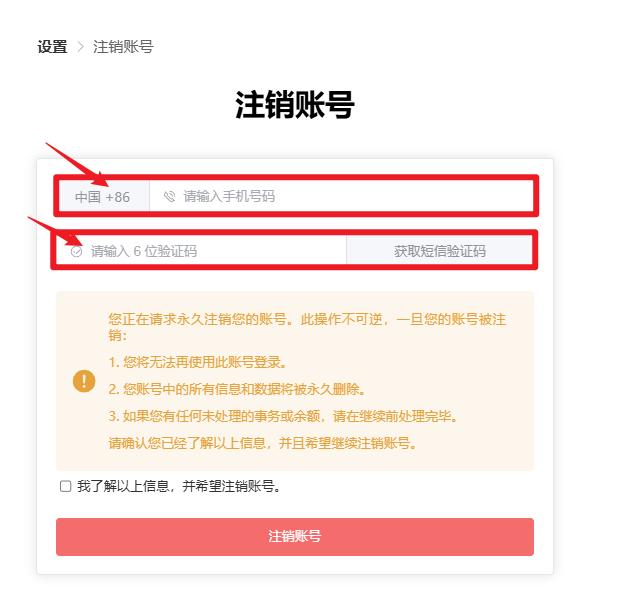
\includegraphics[scale=0.8]{DeleteAccount3.png}
		\caption{用户输入密码}
	\end{figure}

	\item \textbf{代码实现}:
	\begin{minted}[baselinestretch=1]{html}
<template>
...
 <div style='width: 360px; display: flex; flex-direction: column'>
  <!--suppress TypeScriptValidateTypes-->
  <el-popconfirm :title="t('SettingsPage.ConfirmDeleteAccount')"
                 :confirm-button-text="t('SettingsPage.Yes')"
                 :cancel-button-text="t('SettingsPage.No')"
                 :icon='WarningFilled'
                 width='360px'
                 :hide-after='0'
                 icon-color='#F56C6C'
                 @confirm="router.push('/delete-account')">
    <template #reference>
      <!--suppress TypeScriptValidateTypes-->
      <el-button size='large'
                 :icon='Delete'
                 plain
                 type='danger'
                 style='justify-content: flex-start'>
        {{ t('SettingsPage.DeleteAccount') }}
      </el-button>
    </template>
  </el-popconfirm>
 </div>
...
</template>
	\end{minted}
	
	\begin{minted}[baselinestretch=1]{typescript}
<script setup lang='ts'>
	const router = useRouter()
</script>
	\end{minted}

\end{itemize}

\subsubsection{隐私设置}

\begin{itemize}
\item \textbf{界面设计}:
	\begin{figure}[H]
		\centering
		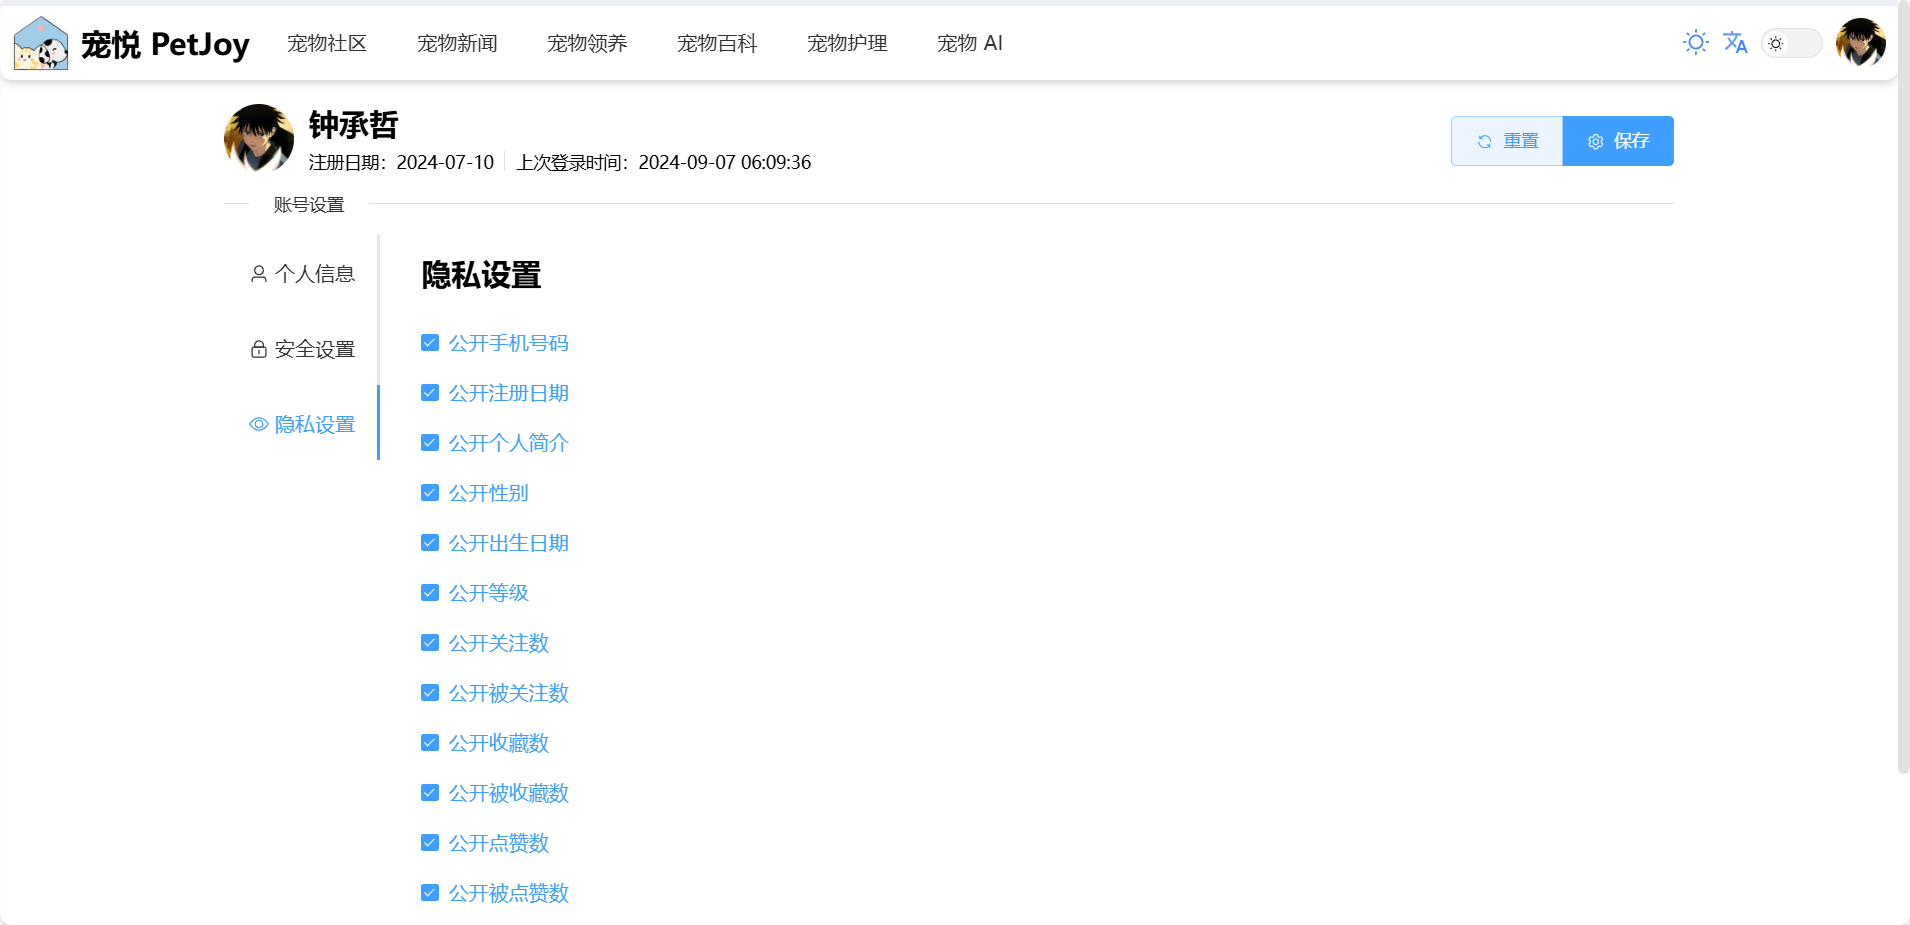
\includegraphics[scale=0.4]{PrivacySettings1.png}
		\caption{隐私设置}
	\end{figure}
	\item \textbf{动作序列}:
	\begin{table}[H]
		\centering
		\renewcommand\arraystretch{1.5}
		\begin{tabular}{|c|>{\raggedright\arraybackslash}p{10cm}|}
			\hline
			\textbf{动作名称} & \textbf{描述} \\ \hline
			\textbf{点击“隐私设置”按钮} & 用户跳转到隐私设置页面。\\ \hline
			\textbf{用户选择隐私设置} & 用户选择自己的隐私设置。\\ \hline
			\textbf{点击“保存”按钮} & 用户保存隐私设置。\\ \hline
		\end{tabular}
	\end{table}

	\item \textbf{用例实现}

	\textbf{点击“隐私设置”按钮}:用户跳转到隐私设置页面。

	\begin{figure}[H]
		\centering
		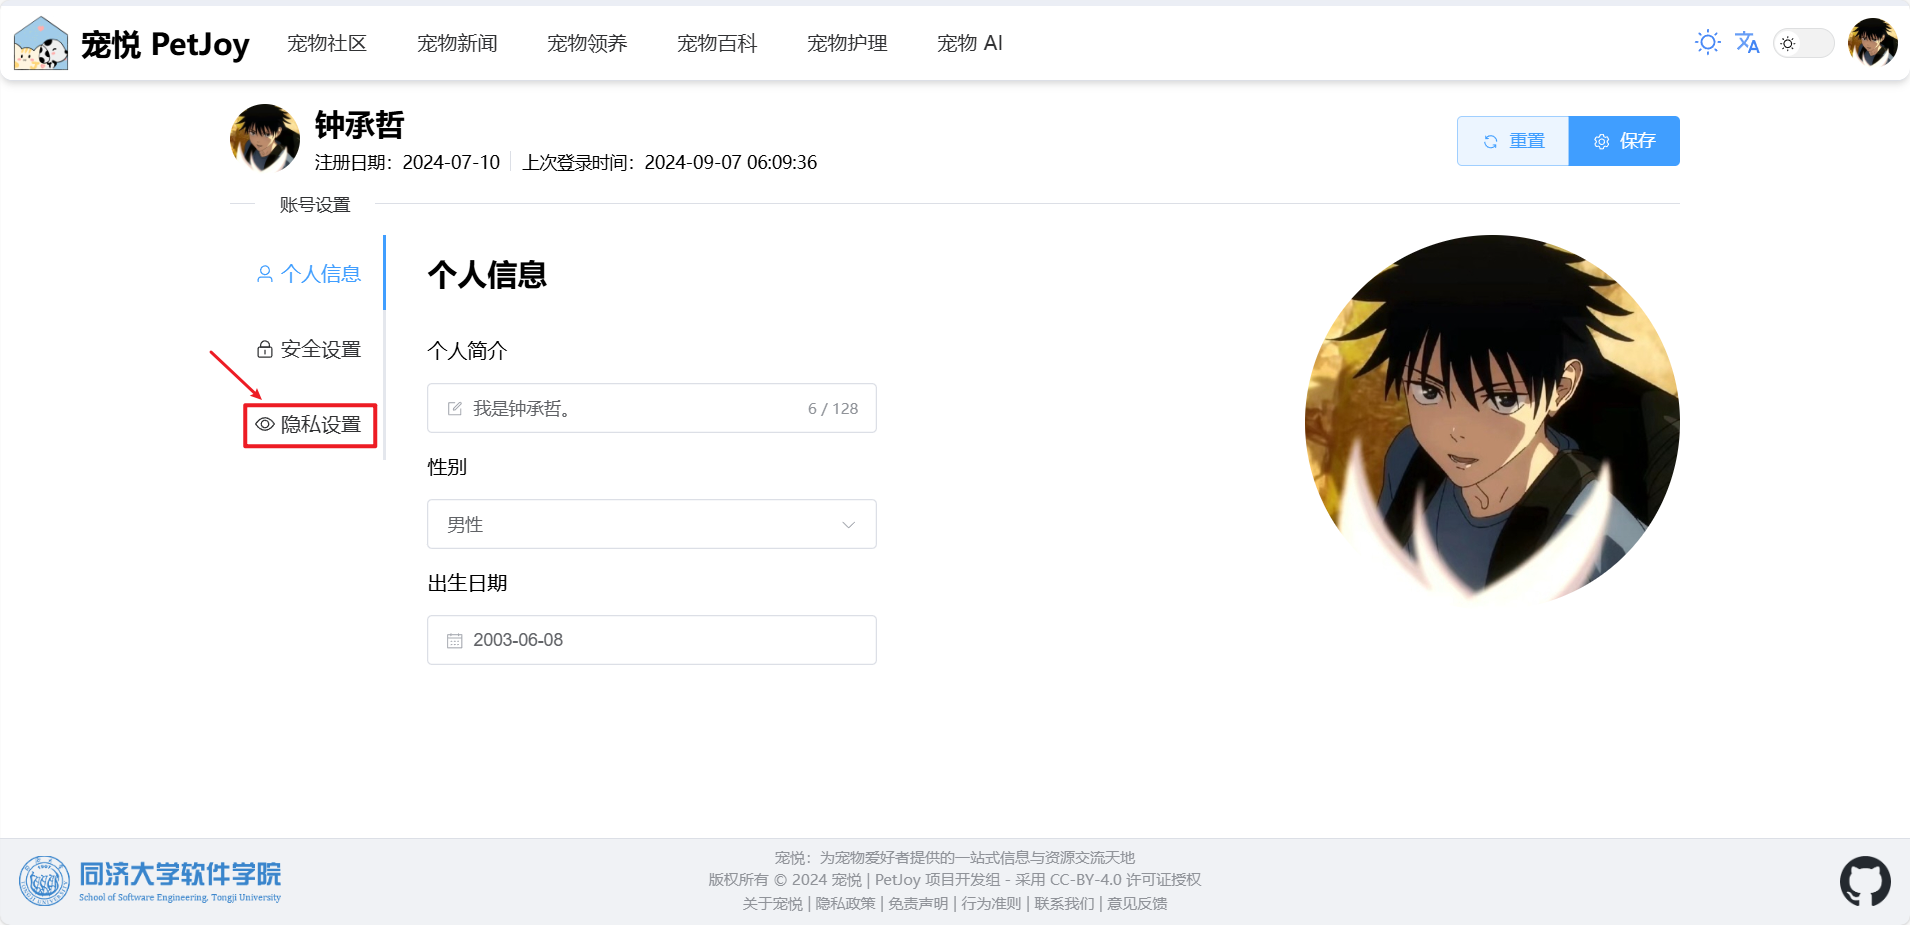
\includegraphics[scale=0.4]{PrivacySettings2.png}
		\caption{用户跳转到隐私设置页面}
	\end{figure}

	\textbf{用户选择隐私设置}:用户选择自己的隐私设置。

	\begin{figure}[H]
		\centering
		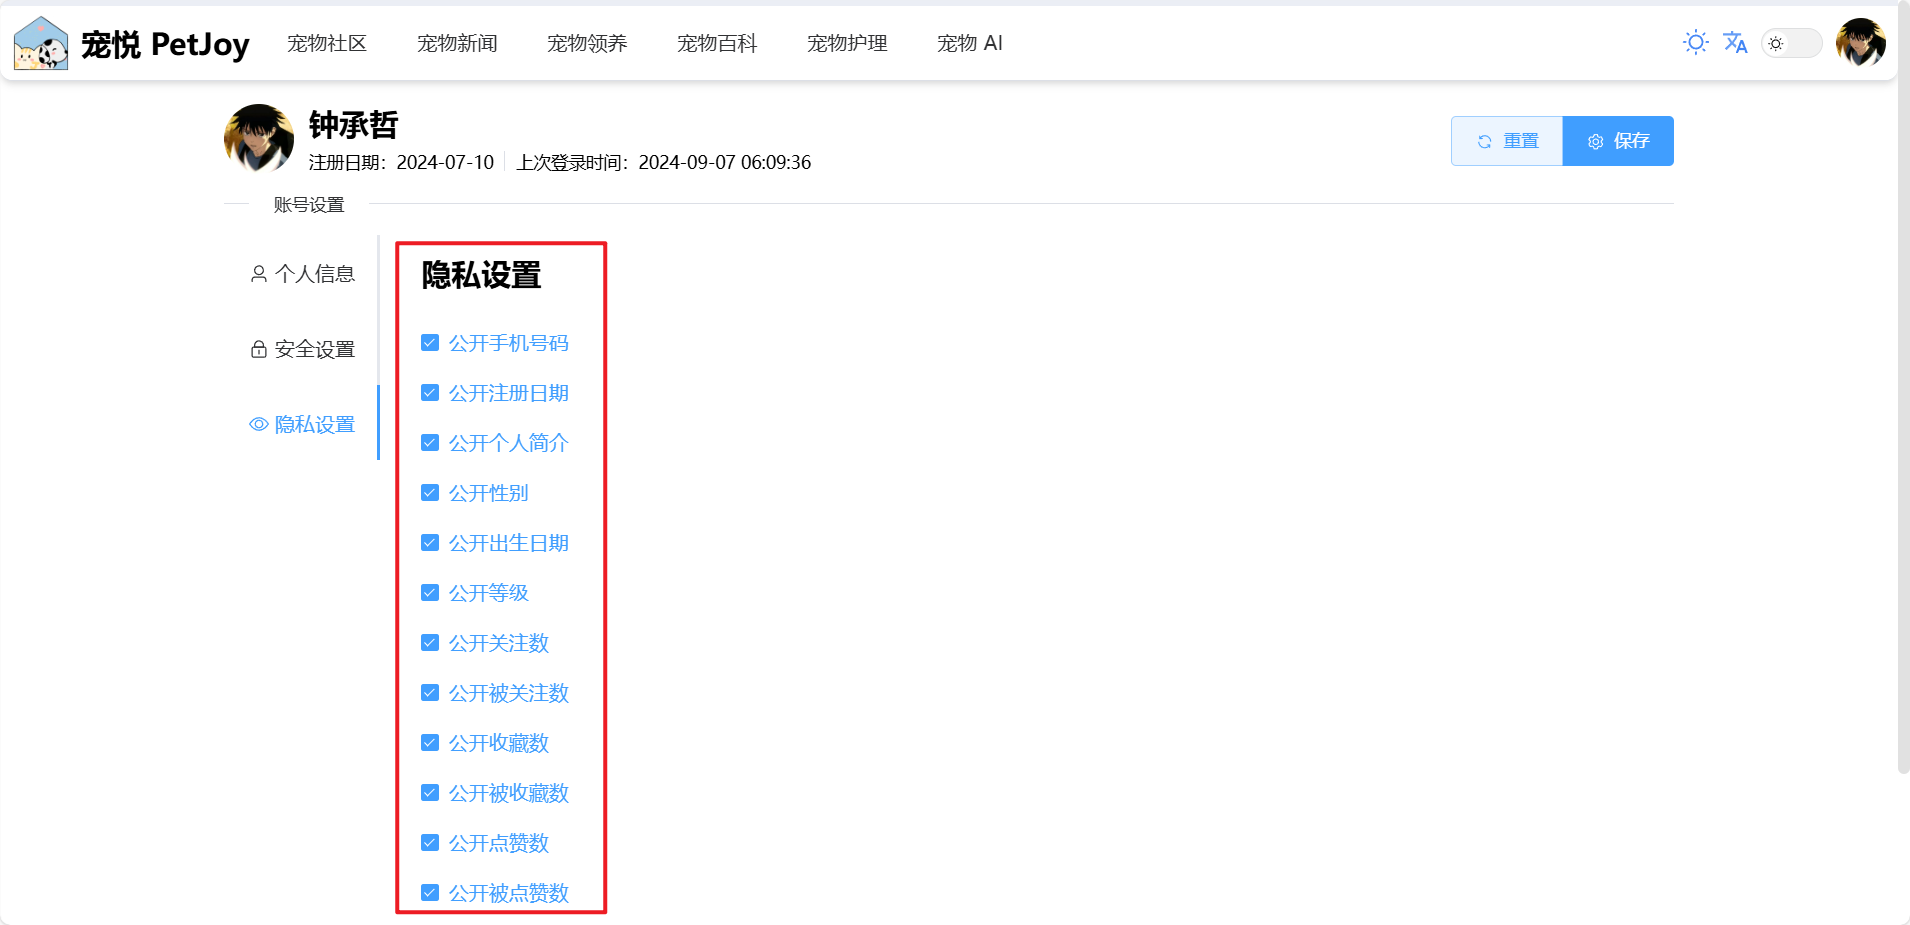
\includegraphics[scale=0.4]{PrivacySettings3.png}
		\caption{用户选择隐私设置}
	\end{figure}

	\textbf{点击“保存”按钮}:用户保存隐私设置。

	\begin{figure}[H]
		\centering
		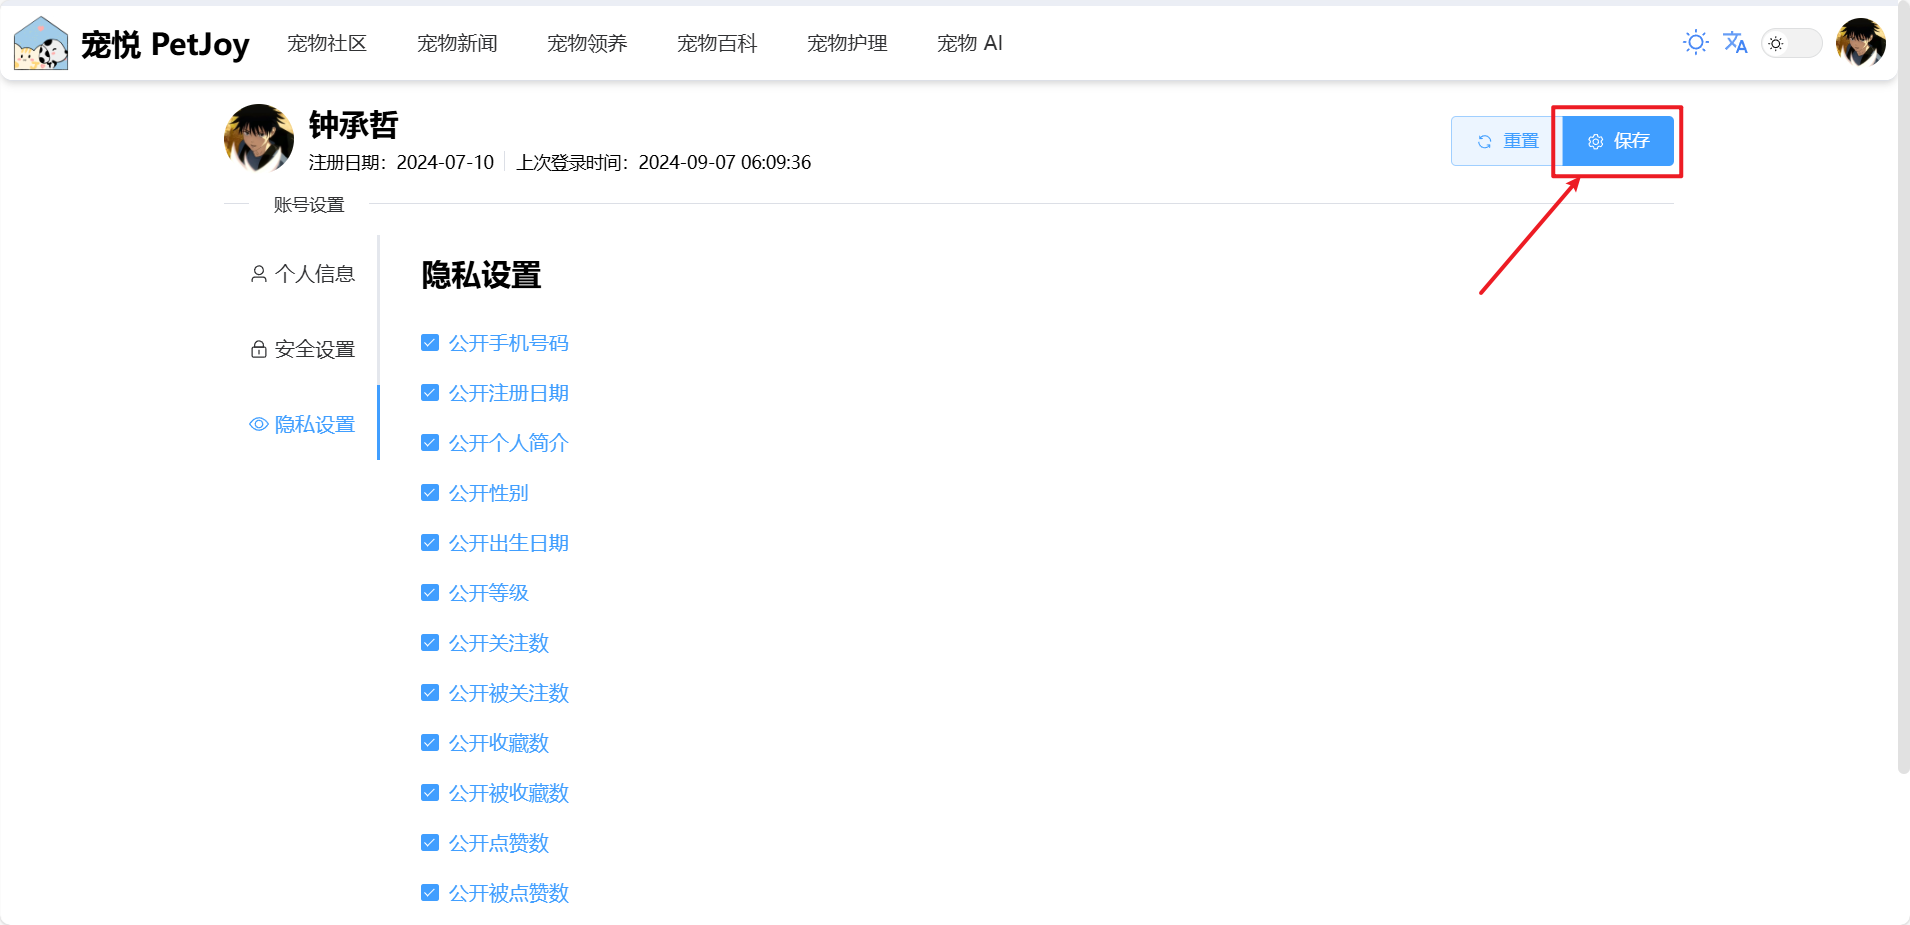
\includegraphics[scale=0.4]{PrivacySettings4.png}
		\caption{用户保存隐私设置}
	\end{figure}

	\item \textbf{代码实现}:
	\begin{minted}[baselinestretch=1]{html}
<template>
...
 <el-tab-pane>
  <template #label>
    <span>
      <el-icon class='icon-align'><View/></el-icon>
      <span>{{ ' ' + t('SettingsPage.PrivacySettings') }}</span>
    </span>
  </template>
	
  <div class='tab-content'>
    <h2>{{ t('SettingsPage.PrivacySettings') }}</h2>
    <div class='checkbox-group'>
      <el-checkbox v-model='userSetting.isTelephonePublic'
                   :label="t('SettingsPage.IsTelephonePublic')"
                   size='large'/>
    ...同上,略
    </div>
  </div>
 </el-tab-pane>
...
</template>
	\end{minted}

\end{itemize}

\subsubsection{账号个人信息}

\paragraph{个人信息展示}

\begin{itemize}
\item \textbf{界面设计}:
	\begin{figure}[H]
		\centering
		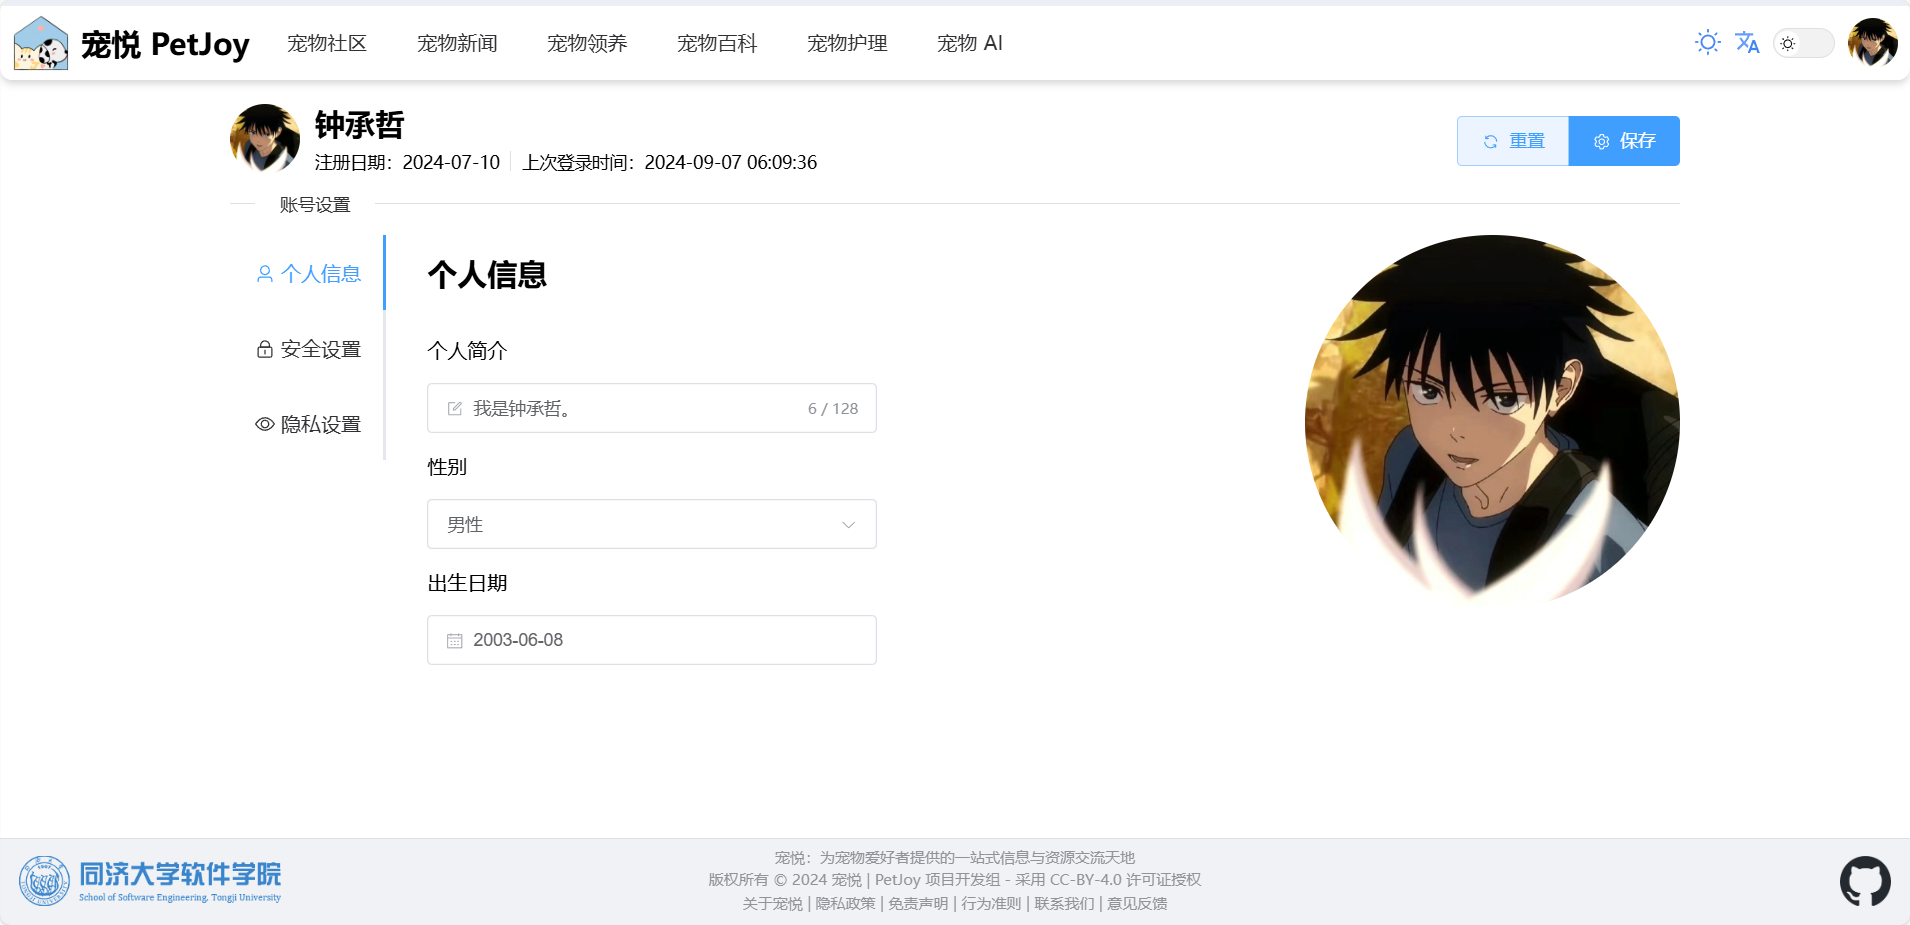
\includegraphics[scale=0.4]{PersonalInformation1.png}
		\caption{个人信息展示}
	\end{figure}
	\item \textbf{动作序列}:
	\begin{table}[H]
		\centering
		\renewcommand\arraystretch{1.5}
		\begin{tabular}{|c|>{\raggedright\arraybackslash}p{10cm}|}
			\hline
			\textbf{动作名称} & \textbf{描述} \\ \hline
			\textbf{点击“个人信息”按钮} & 用户跳转到个人信息页面。\\ \hline
			\textbf{用户查看个人信息} & 用户查看自己的个人信息。\\ \hline
		\end{tabular}
	\end{table}

	\item \textbf{用例实现}

	\textbf{点击“个人信息”按钮}:用户跳转到个人信息页面。

	\begin{figure}[H]
		\centering
		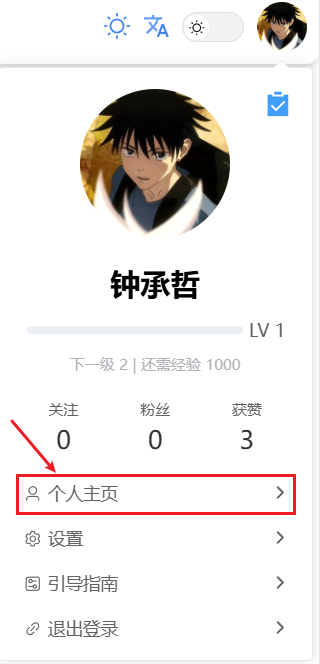
\includegraphics[scale=0.8]{PersonalInformation2.png}
		\caption{用户跳转到个人信息页面}
	\end{figure}

	\textbf{用户查看个人信息}:用户查看自己的个人信息。

	\begin{figure}[H]
		\centering
		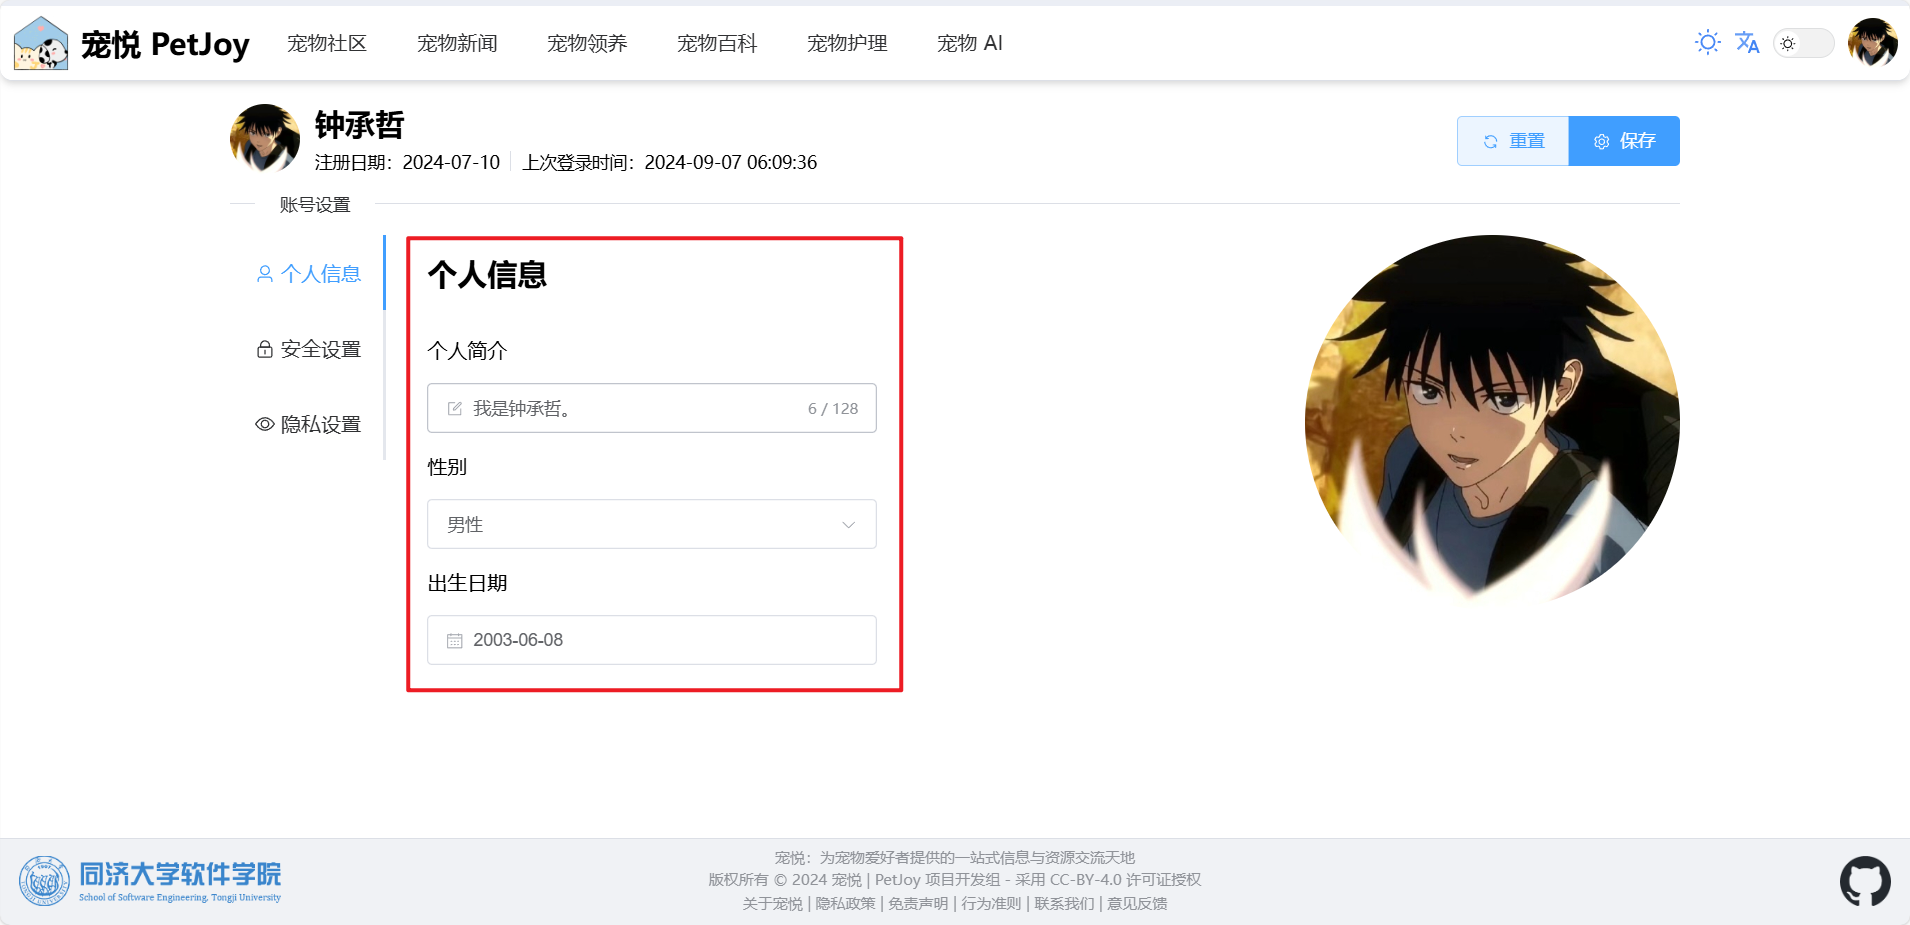
\includegraphics[scale=0.4]{PersonalInformation3.png}
		\caption{用户查看个人信息}
	\end{figure}

	\item \textbf{代码实现}:
	\begin{minted}[baselinestretch=1]{html}
<template>
...
 <el-tab-pane>
  <template #label>
    <span>
      <el-icon class='icon-align'><User/></el-icon>
      <span>{{ ' ' + t('SettingsPage.PersonalInformation') }}</span>
    </span>
  </template>
	
  <div class='tab-content'>
    <h2>{{ t('SettingsPage.PersonalInformation') }}</h2>
	
    <p>{{ t('SettingsPage.Profile') }}</p>
    <!--suppress TypeScriptValidateTypes-->
    <el-input v-model='user.profile'
              size='large'
              maxlength='128'
              style='width: 360px'
              :prefix-icon='Edit'
              :placeholder="t('SettingsPage.ProfilePrompt')"
              autocomplete='off'
              show-word-limit/>
    <p>{{ t('SettingsPage.Gender') }}</p>
    <el-select v-model='user.gender'
               size='large'
               :placeholder="t('SettingsPage.GenderPrompt')"
               style='width: 360px'>
      <el-option :label="t('SettingsPage.Male')" :value='0'/>
      <el-option :label="t('SettingsPage.Female')" :value='1'/>
    </el-select>
    <p>{{ t('SettingsPage.Birthdate') }}</p>
    <el-date-picker v-model='user.birthdate'
                    type='date'
                    :disabled-date='disabledDate'
                    style='width: 360px'
                    size='large'
                    :placeholder="t('SettingsPage.BirthdatePrompt')"
                    :editable='false'
                    :clearable='false'/>
	
    <div @click='showAvatarCropper=true' class='avatar-wrapper'>
      <el-avatar :src='`${ossBaseUrl}${user.avatarUrl}`' class='avatar-image'>
        <el-icon :size='150'>
          <Avatar/>
        </el-icon>
      </el-avatar>
      <div class='avatar-overlay'>
        <span class='upload-text'>{{ t('AvatarCropper.UploadAvatar') }}</span>
      </div>
    </div>
  </div>
 </el-tab-pane>
...
</template>
	\end{minted}

\end{itemize}

\paragraph{个人信息修改}

\begin{itemize}
\item \textbf{界面设计}:
	\begin{figure}[H]
		\centering
		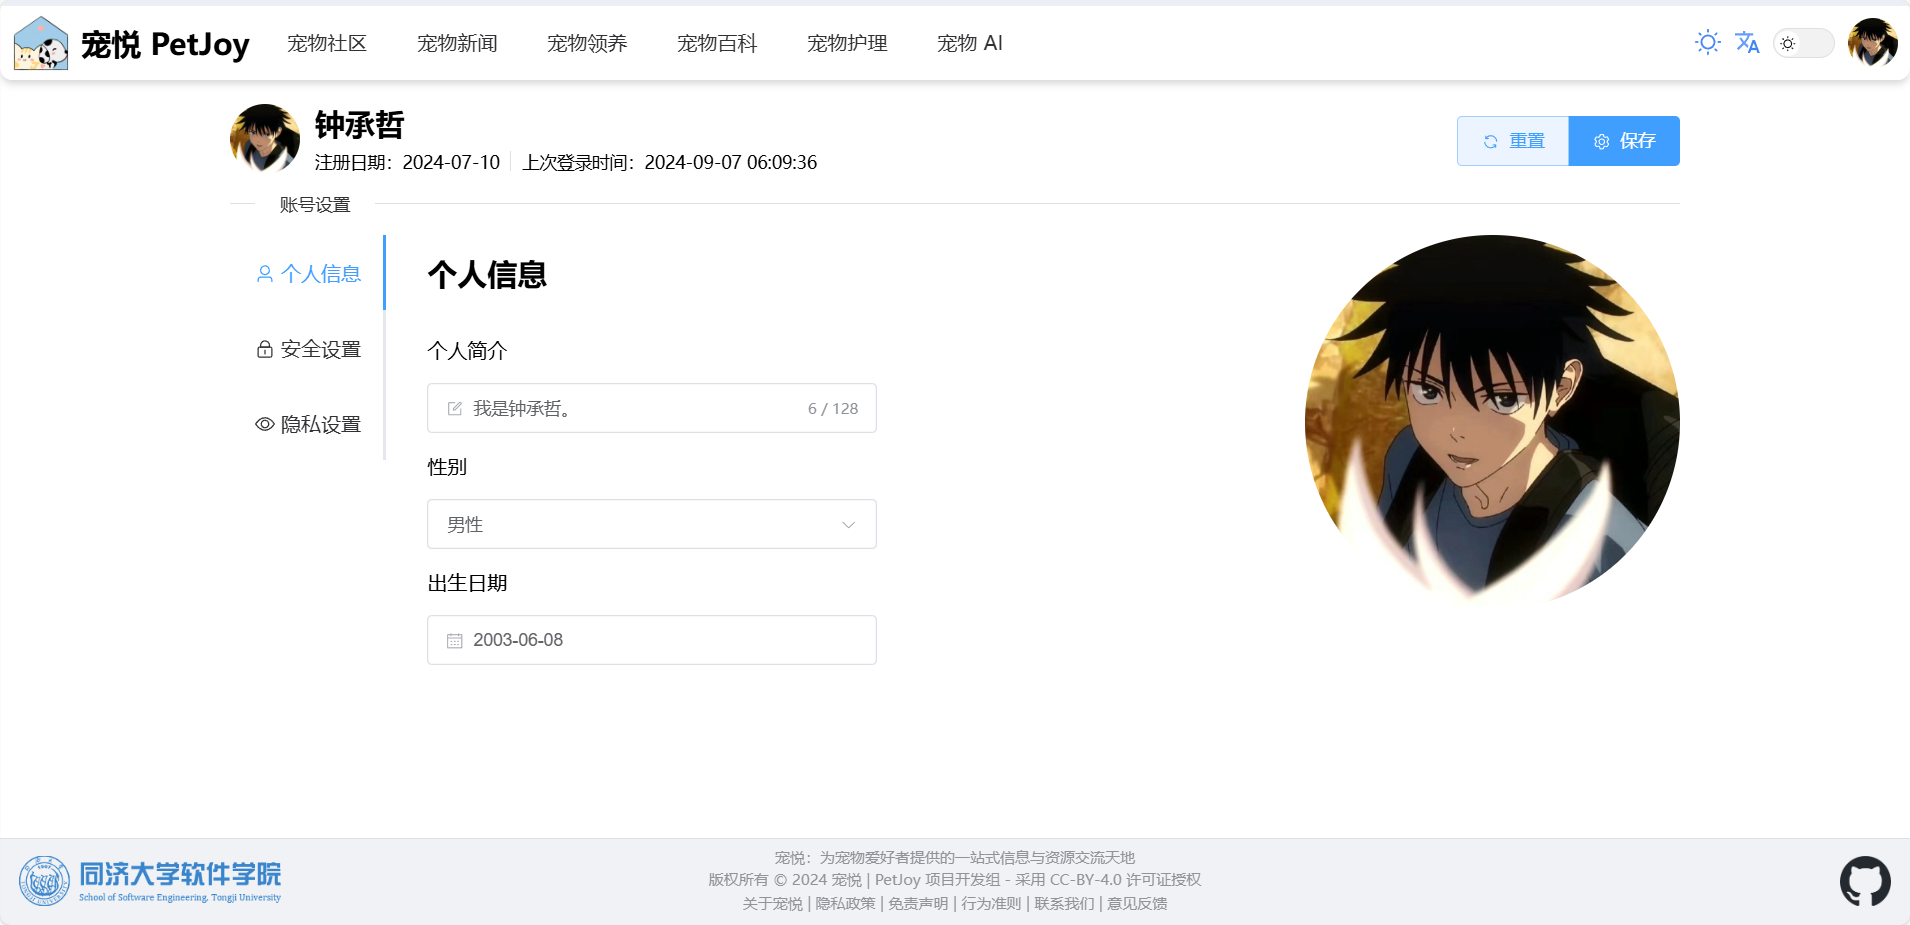
\includegraphics[scale=0.4]{PersonalInformation1.png}
		\caption{个人信息修改}
	\end{figure}
	\item \textbf{动作序列}:
	\begin{table}[H]
		\centering
		\renewcommand\arraystretch{1.5}
		\begin{tabular}{|c|>{\raggedright\arraybackslash}p{10cm}|}
			\hline
			\textbf{动作名称} & \textbf{描述} \\ \hline
			\textbf{点击“修改个人信息”按钮} & 用户跳转到修改个人信息页面。\\ \hline
			\textbf{用户修改个人信息} & 用户修改自己的个人信息。\\ \hline
			\textbf{点击“保存”按钮} & 用户保存修改的个人信息。\\ \hline
		\end{tabular}
	\end{table}

	\item \textbf{用例实现}

	\textbf{点击“个人信息”按钮}:用户跳转到修改个人信息页面。

	\begin{figure}[H]
		\centering
		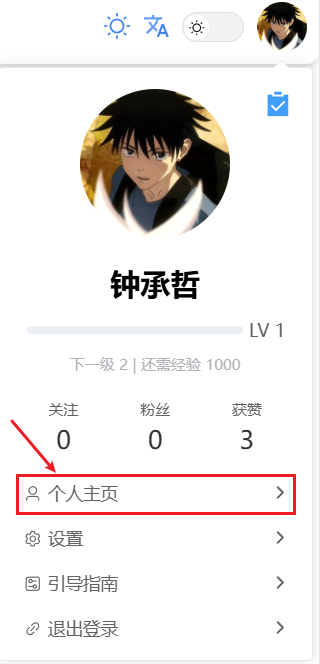
\includegraphics[scale=0.8]{PersonalInformation2.png}
		\caption{用户跳转到修改个人信息页面}
	\end{figure}

	\textbf{用户修改个人信息}:用户修改自己的个人信息。

	\begin{figure}[H]
		\centering
		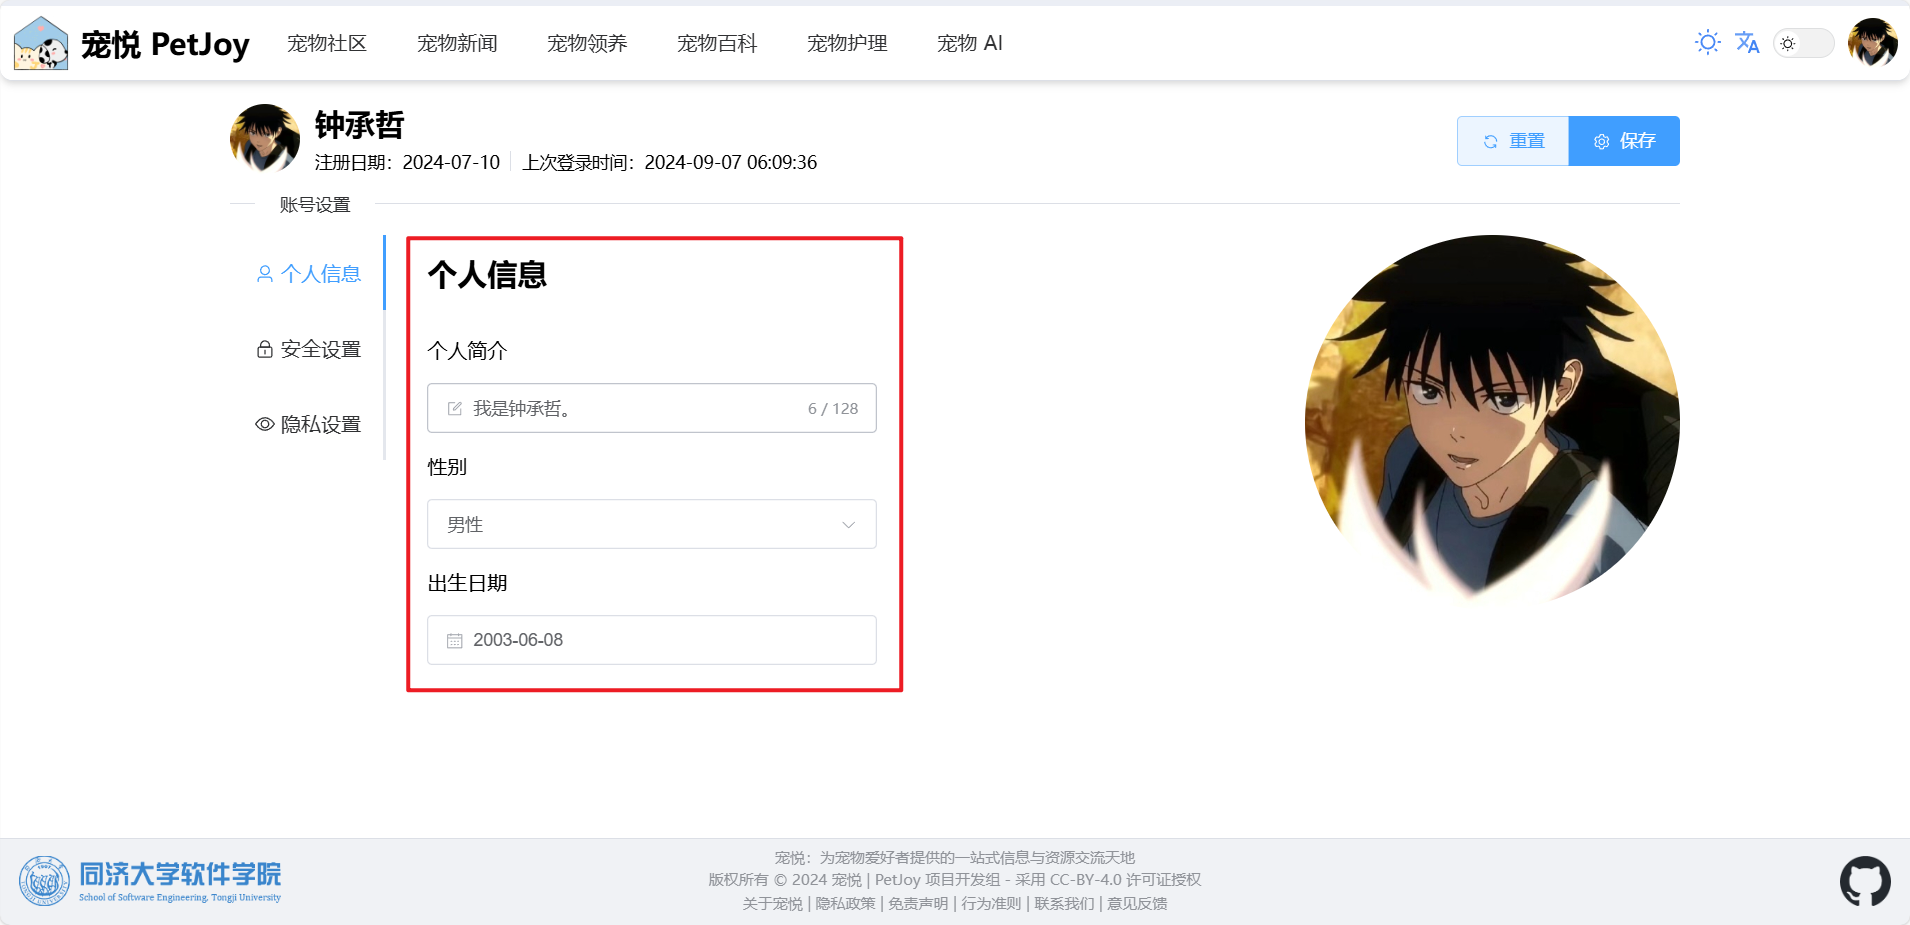
\includegraphics[scale=0.4]{PersonalInformation3.png}
		\caption{用户修改个人信息}
	\end{figure}

	\textbf{点击“保存”按钮}:用户保存修改的个人信息。

	\begin{figure}[H]
		\centering
		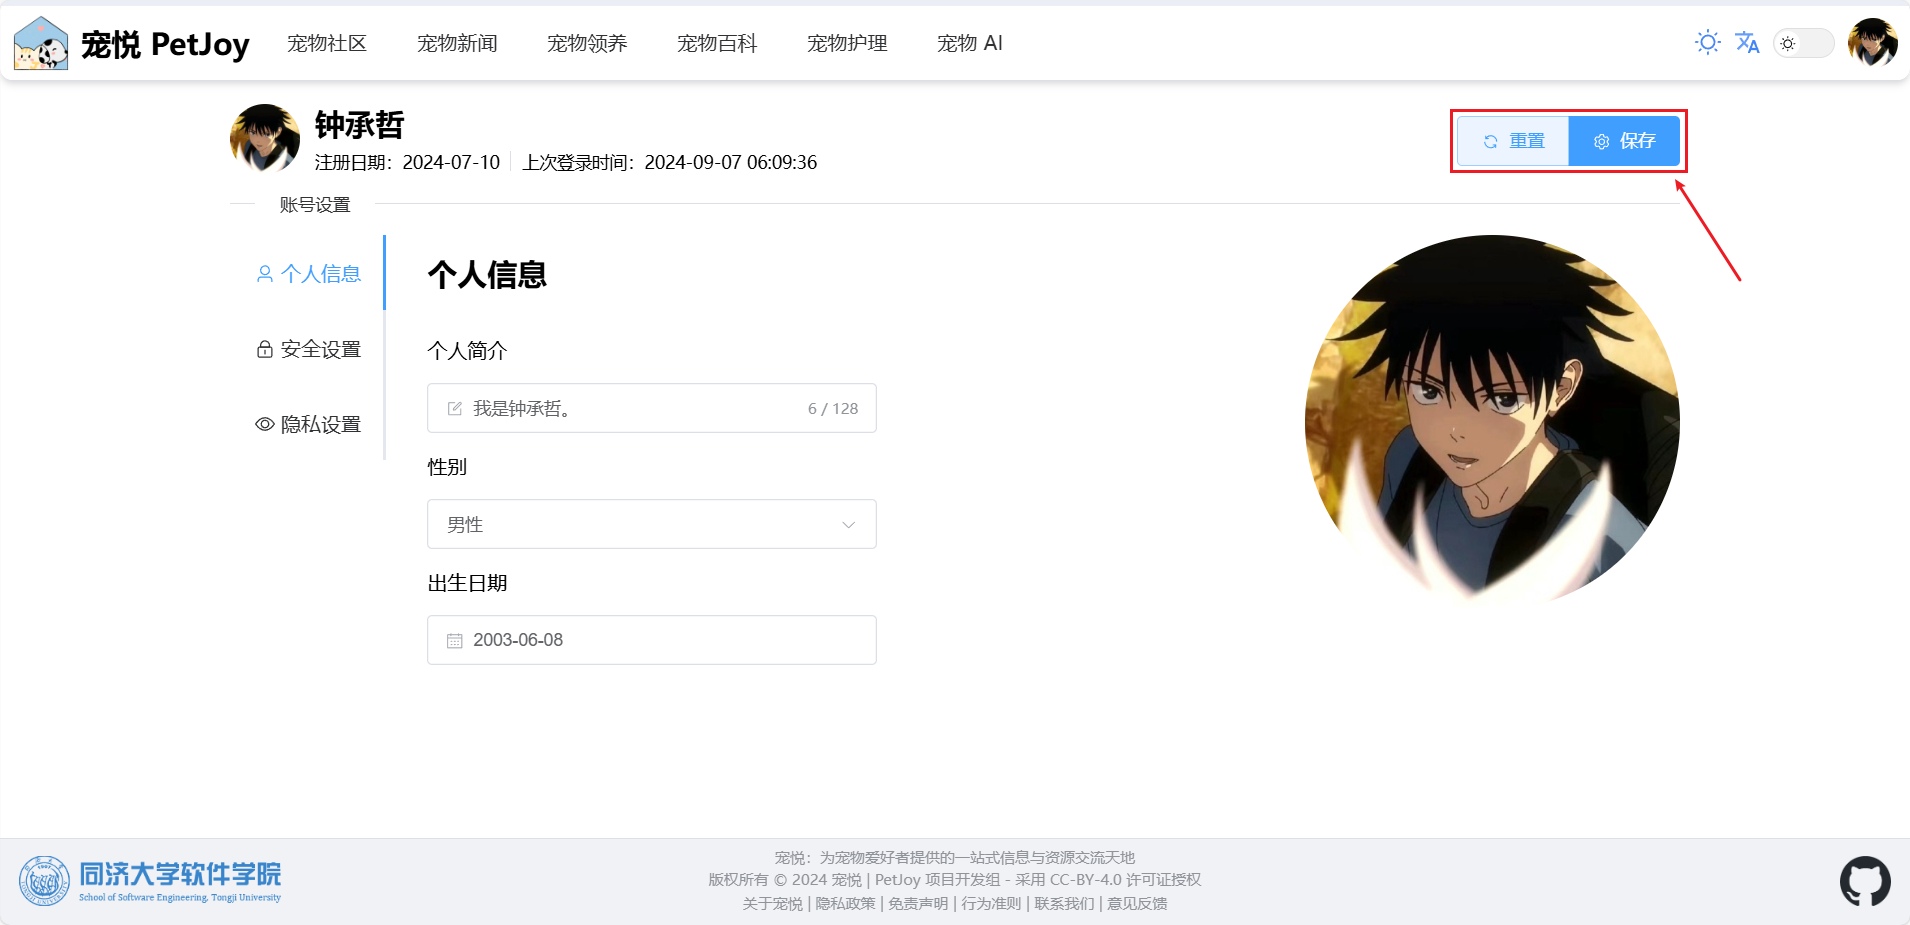
\includegraphics[scale=0.4]{PersonalInformation4.png}
		\caption{用户保存修改的个人信息}
	\end{figure}

	\item \textbf{代码实现}:
	\begin{minted}[baselinestretch=1]{html}
<template>
...
 <el-button-group style='margin-top: 28px'>
  <!--suppress TypeScriptValidateTypes-->
  <el-button type='primary' plain size='large' :icon='Refresh' @click='resetSettings'>{{
			t('SettingsPage.Reset')
	}}
  </el-button>
  <!--suppress TypeScriptValidateTypes-->
  <el-button type='primary' size='large' :icon='Setting' @click='saveSettings'>{{
			t('SettingsPage.Save')
	}}
  </el-button>
 </el-button-group>
...
</template>
	\end{minted}

\end{itemize}

\subsection{管理员子系统}

\subsubsection{帖子举报管理}

\begin{itemize}
	\item \textbf{界面设计}:
	\begin{figure}[H]
		\centering
		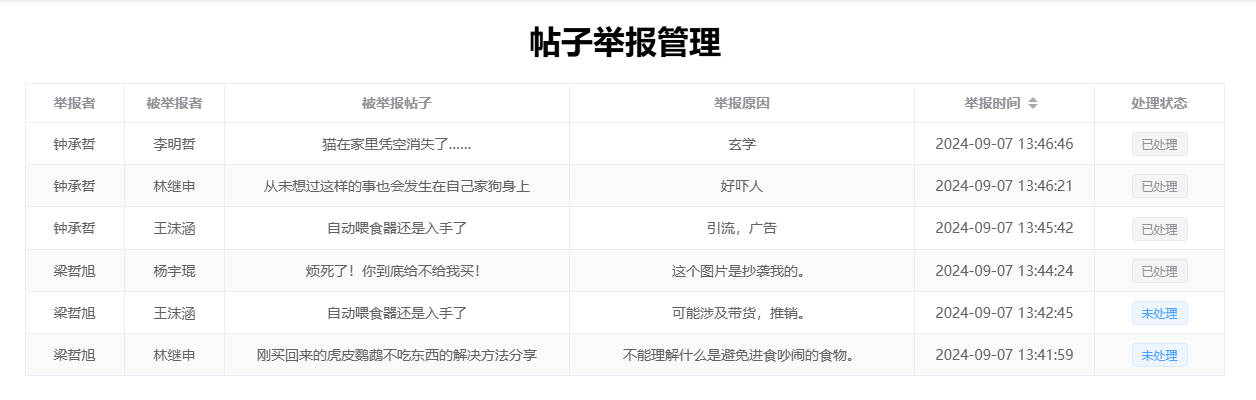
\includegraphics[scale=0.3]{PostReportManagementUI.jpg}
		\caption{帖子举报管理}
	\end{figure}
	\item \textbf{动作序列}:
	\begin{table}[H]
		\centering
		\renewcommand\arraystretch{1.5}
		\begin{tabular}{|c|>{\raggedright\arraybackslash}p{10cm}|}
			\hline
			\textbf{动作名称} & \textbf{描述} \\ \hline
			\textbf{查看被举报的帖子信息} & 管理员可以查看被举报的帖子信息,包括举报原因、举报时间等。\\ \hline
			\textbf{按时间顺序排列被举报的帖子} & 被举报的帖子可以根据举报时间排序,方便管理员优先处理较早的举报。\\ \hline
			\textbf{更改帖子处理状态} & 管理员在处理完举报后,可以将该帖子的处理状态从“未处理”更改为“已处理”,以便记录处理结果。\\ \hline
		\end{tabular}
	\end{table}
	
	\item \textbf{用例实现}
	
	\textbf{查看被举报的帖子信息}:管理员可以在举报管理界面中查看被举报的帖子详情,包括举报原因、举报时间等。
	
	\begin{figure}[H]
		\centering
		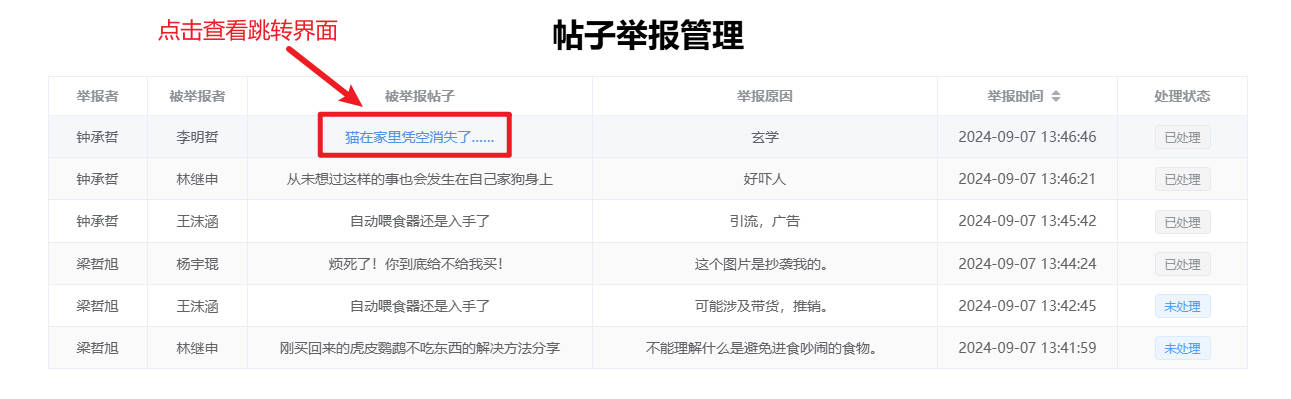
\includegraphics[scale=0.3]{ViewReportedPostDetails.jpg}
		\caption{查看被举报的帖子信息}
	\end{figure}
	
	\textbf{按时间顺序排列被举报的帖子}:系统可以按举报时间将帖子列表排序,管理员可以清晰地看到哪条帖子被举报的时间较早。
	
	\begin{figure}[H]
		\centering
		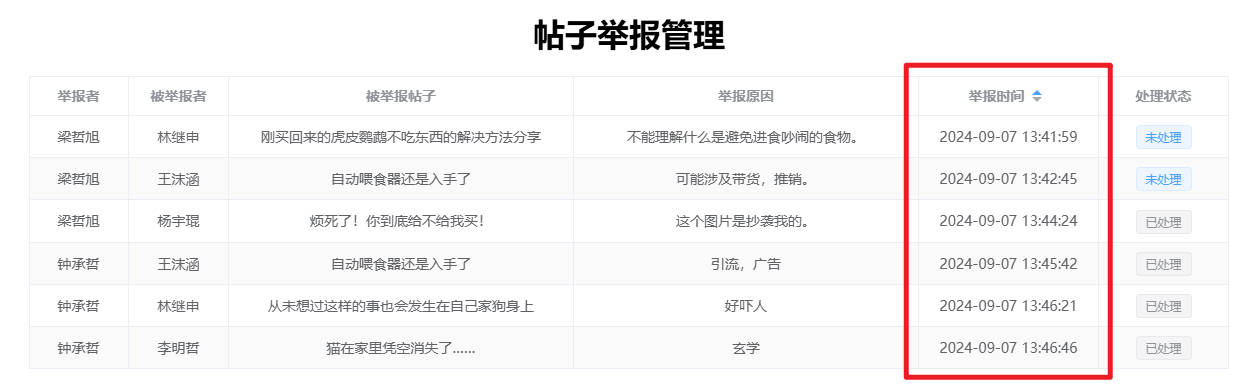
\includegraphics[scale=0.3]{SortReportedPostsByTime.jpg}
		\caption{按时间顺序排列被举报的帖子}
	\end{figure}
	
	\textbf{更改帖子处理状态}:管理员在处理完举报后,可以将帖子的状态从“未处理”改为“已处理”。
	
	\begin{figure}[H]
		\centering
		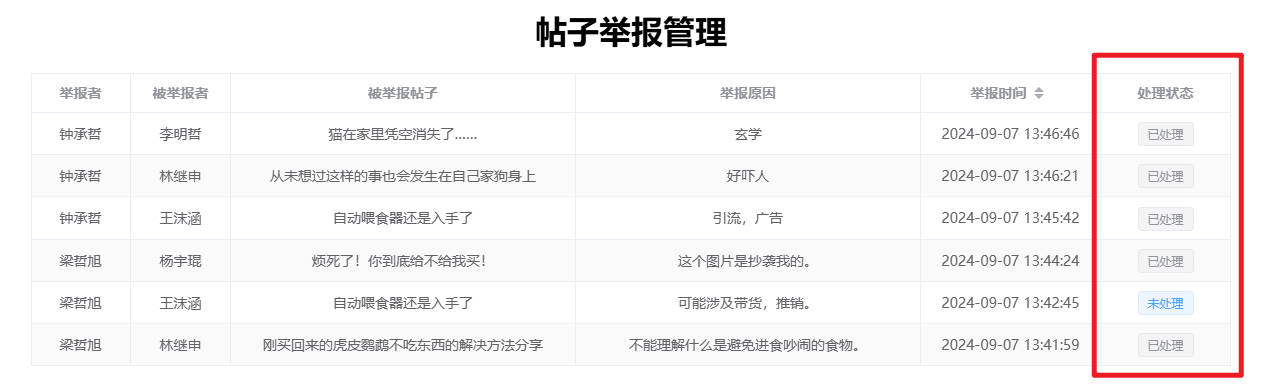
\includegraphics[scale=0.3]{ChangePostStatus.jpg}
		\caption{更改帖子处理状态}
	\end{figure}
	
	\item \textbf{代码实现}:
	
\end{itemize}

\subsubsection{帖子评论举报管理}

\begin{itemize}
	\item \textbf{界面设计}:
	\begin{figure}[H]
		\centering
		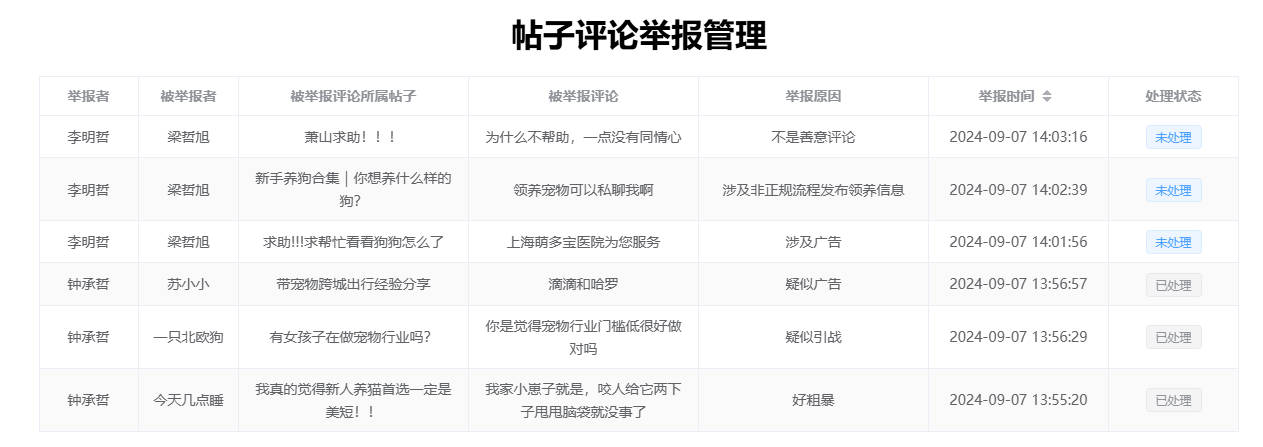
\includegraphics[scale=0.3]{PostCommentReportManagementUI.jpg}
		\caption{帖子评论举报管理}
	\end{figure}
	\item \textbf{动作序列}:
	\begin{table}[H]
		\centering
		\renewcommand\arraystretch{1.5}
		\begin{tabular}{|c|>{\raggedright\arraybackslash}p{10cm}|}
			\hline
			\textbf{动作名称} & \textbf{描述} \\ \hline
			\textbf{查看被举报的帖子评论信息} & 管理员可以查看被举报的帖子评论信息,包括举报原因、举报时间等。\\ \hline
			\textbf{按时间顺序排列被举报的帖子评论} & 被举报的帖子评论可以根据举报时间排序,方便管理员优先处理较早的举报。\\ \hline
			\textbf{更改帖子评论处理状态} & 管理员在处理完举报后,可以将该评论的处理状态从“未处理”更改为“已处理”,以便记录处理结果。\\ \hline
		\end{tabular}
	\end{table}
	
	\item \textbf{用例实现}
	
	\textbf{查看被举报的帖子评论信息}:管理员可以在举报管理界面中查看被举报的帖子评论详情,包括举报原因、举报时间等。
	
	\begin{figure}[H]
		\centering
		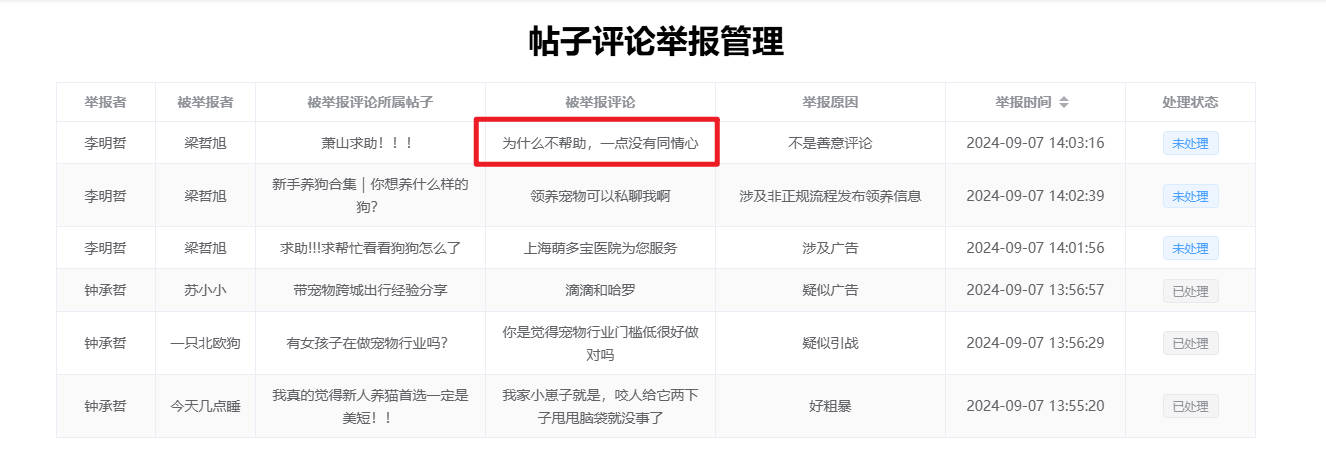
\includegraphics[scale=0.3]{ViewReportedPostCommentDetails.jpg}
		\caption{查看被举报的帖子评论信息}
	\end{figure}
	
	\textbf{按时间顺序排列被举报的帖子评论}:系统可以按举报时间将评论列表排序,管理员可以清晰地看到哪条评论被举报的时间较早。
	
	\begin{figure}[H]
		\centering
		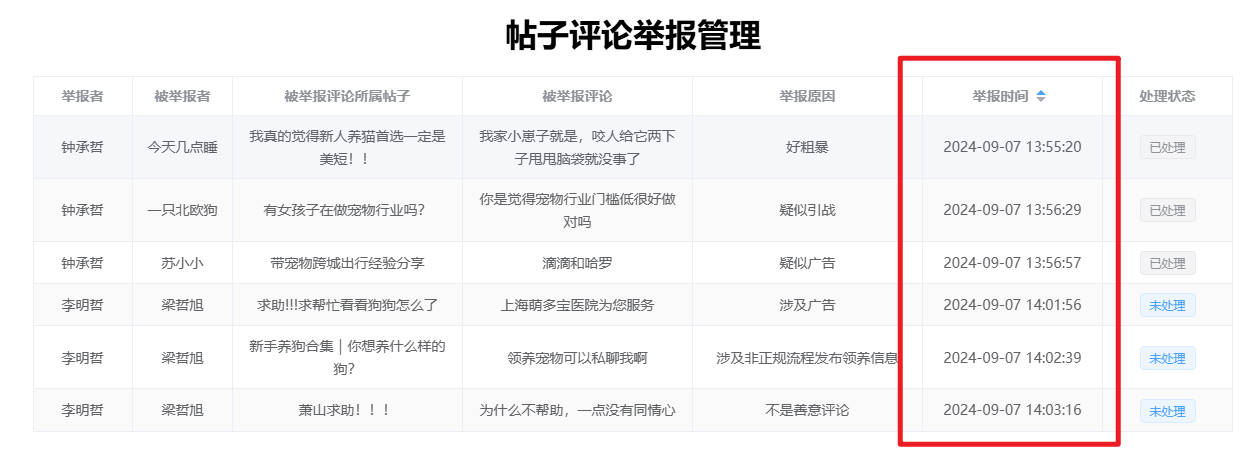
\includegraphics[scale=0.3]{SortReportedPostCommentsByTime.jpg}
		\caption{按时间顺序排列被举报的帖子评论}
	\end{figure}
	
	\textbf{更改帖子评论处理状态}:管理员在处理完举报后,可以将评论的状态从“未处理”改为“已处理”。
	
	\begin{figure}[H]
		\centering
		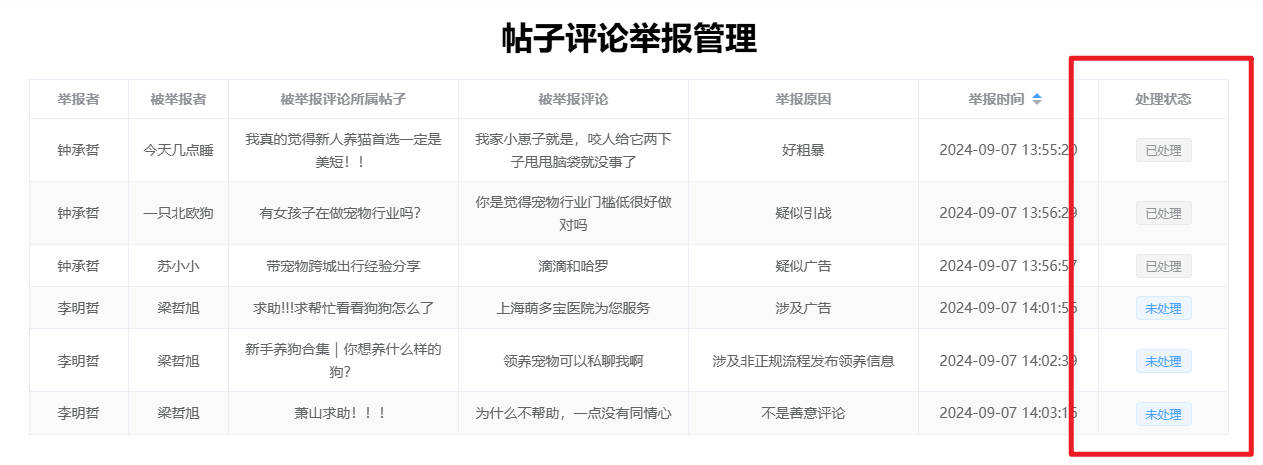
\includegraphics[scale=0.3]{ChangePostCommentStatus.jpg}
		\caption{更改帖子评论处理状态}
	\end{figure}
	
	\item \textbf{代码实现}:
	
\end{itemize}

\subsubsection{新闻评论举报管理}

\begin{itemize}
	\item \textbf{界面设计}:
	\begin{figure}[H]
		\centering
		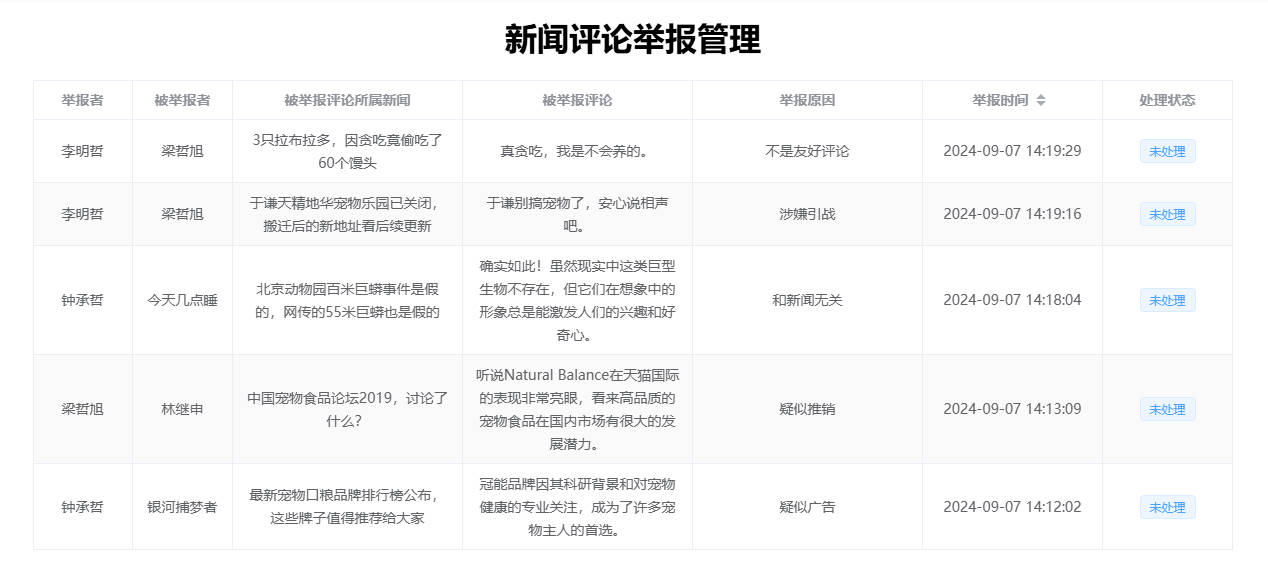
\includegraphics[scale=0.3]{NewsCommentReportManagementUI.jpg}
		\caption{新闻评论举报管理}
	\end{figure}
	\item \textbf{动作序列}:
	\begin{table}[H]
		\centering
		\renewcommand\arraystretch{1.5}
		\begin{tabular}{|c|>{\raggedright\arraybackslash}p{10cm}|}
			\hline
			\textbf{动作名称} & \textbf{描述} \\ \hline
			\textbf{查看被举报的新闻评论信息} & 管理员可以查看被举报的新闻评论信息,包括举报原因、举报时间等。\\ \hline
			\textbf{按时间顺序排列被举报的新闻评论} & 被举报的新闻评论可以根据举报时间排序,方便管理员优先处理较早的举报。\\ \hline
			\textbf{更改新闻评论处理状态} & 管理员在处理完举报后,可以将该评论的处理状态从“未处理”更改为“已处理”,以便记录处理结果。\\ \hline
		\end{tabular}
	\end{table}
	
	\item \textbf{用例实现}
	
	\textbf{查看被举报的新闻评论信息}:管理员可以在举报管理界面中查看被举报的新闻评论详情,包括举报原因、举报时间等。
	
	\begin{figure}[H]
		\centering
		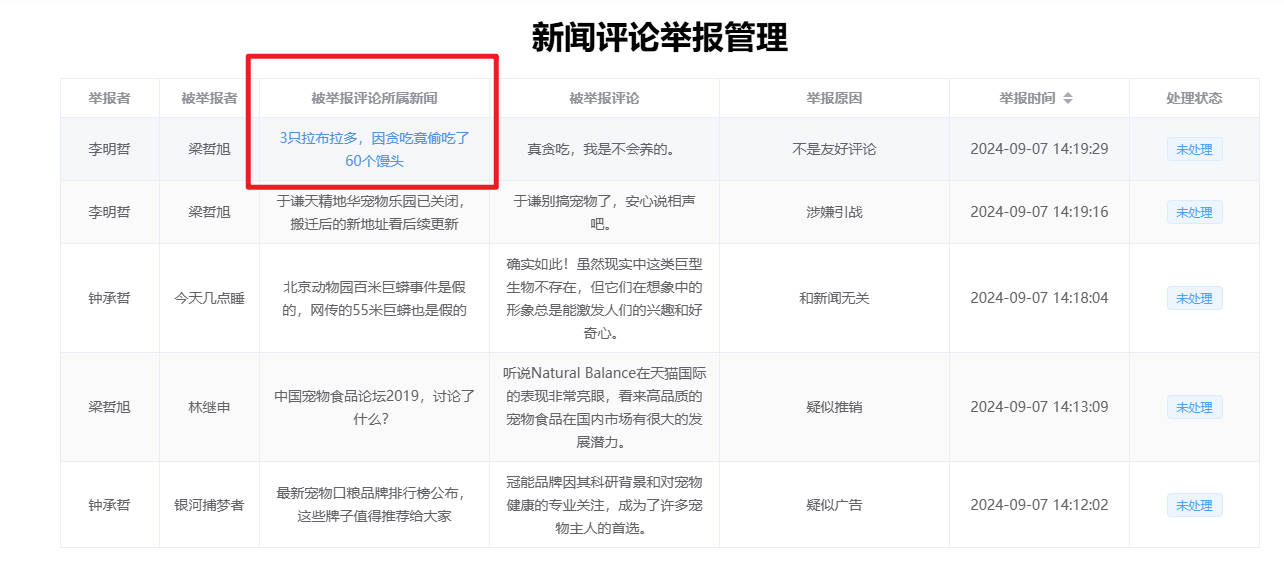
\includegraphics[scale=0.3]{ViewReportedNewsCommentDetails.jpg}
		\caption{查看被举报的新闻评论信息}
	\end{figure}
	
	\textbf{按时间顺序排列被举报的新闻评论}:系统可以按举报时间将评论列表排序,管理员可以清晰地看到哪条评论被举报的时间较早。
	
	\begin{figure}[H]
		\centering
		\includegraphics[scale=0.3]{SortReportedNewsCommentsByTime.jpg}
		\caption{按时间顺序排列被举报的新闻评论}
	\end{figure}
	
	\textbf{更改新闻评论处理状态}:管理员在处理完举报后,可以将评论的状态从“未处理”改为“已处理”。
	
	\begin{figure}[H]
		\centering
		\includegraphics[scale=0.3]{ChangeNewsCommentStatus.jpg}
		\caption{更改新闻评论处理状态}
	\end{figure}
	
	\item \textbf{代码实现}:
	
\end{itemize}

\subsubsection{新闻管理}

\begin{itemize}
	\item \textbf{界面设计}:
	\begin{figure}[H]
		\centering
		\includegraphics[scale=0.3]{NewsManagementUI.jpg}
		\caption{新闻管理}
	\end{figure}
	\item \textbf{动作序列}:
	\begin{table}[H]
		\centering
		\renewcommand\arraystretch{1.5}
		\begin{tabular}{|c|>{\raggedright\arraybackslash}p{10cm}|}
			\hline
			\textbf{动作名称} & \textbf{描述} \\ \hline
			\textbf{查看新闻列表} & 管理员查看发布的所有新闻的列表。\\ \hline
			\textbf{点击“预览”按钮} & 管理员点击某个新闻的“预览”按钮,查看新闻的详细信息。\\ \hline
			\textbf{点击“编辑”按钮} & 管理员点击某个新闻的“编辑”按钮,进入编辑界面对新闻内容进行修改。\\ \hline
			\textbf{点击“删除”按钮} & 管理员点击“删除”按钮,移除某条新闻。\\ \hline
		\end{tabular}
	\end{table}
	
	\item \textbf{用例实现}
	
	\textbf{查看新闻列表}:管理员可以在新闻管理页面中查看发布的所有新闻。
	
	\textbf{点击“预览”按钮}:管理员点击某个新闻的“预览”按钮,查看该新闻的详细内容。
	
	\begin{figure}[H]
		\centering
		\includegraphics[scale=0.3]{PreviewNews.jpg}
		\caption{点击“预览”按钮}
	\end{figure}
	
	\textbf{点击“编辑”按钮}:管理员点击“编辑”按钮,进入编辑界面对该新闻内容进行修改。
	
	\begin{figure}[H]
		\centering
		\includegraphics[scale=0.3]{EditNews.jpg}
		\caption{点击“编辑”按钮}
	\end{figure}
	
	\textbf{点击“删除”按钮}:管理员选择符合删除标准的新闻,点击“删除”按钮,新闻将被删除。
	
	\begin{figure}[H]
		\centering
		\includegraphics[scale=0.3]{DeleteNews.jpg}
		\caption{点击“删除”按钮}
	\end{figure}
	
	\item \textbf{代码实现}:
	
\end{itemize}

\subsubsection{用户反馈管理}

\begin{itemize}
	\item \textbf{界面设计}:
	\begin{figure}[H]
		\centering
		\includegraphics[scale=0.4]{UserFeedbackManagementUI.png}
		\caption{用户反馈管理}
	\end{figure}
	\item \textbf{动作序列}:
	\begin{table}[H]
		\centering
		\renewcommand\arraystretch{1.5}
		\begin{tabular}{|c|>{\raggedright\arraybackslash}p{10cm}|}
			\hline
			\textbf{动作名称} & \textbf{描述} \\ \hline
			\textbf{查看用户反馈信息} & 管理员可以查看用户提交的反馈信息,包括反馈类型、反馈内容、提交时间以及用户的联系方式(如果提供)。\\ \hline
			\textbf{按时间顺序排列用户反馈} & 用户反馈可以按照提交时间排序,管理员可以优先处理较早的反馈。\\ \hline
			\textbf{更改用户反馈处理状态} & 管理员在处理完反馈后,可以将该反馈的状态从“未处理”改为“已处理”,记录处理结果。\\ \hline
		\end{tabular}
	\end{table}
	
	\item \textbf{用例实现}
	
	\textbf{查看用户反馈信息}:管理员可以在反馈管理界面中查看用户提交的反馈详情,具体包括反馈内容、反馈类型以及用户提交的时间。
	
	\begin{figure}[H]
		\centering
		\includegraphics[scale=0.3]{ViewUserFeedbackDetails.png}
		\caption{查看用户反馈信息}
	\end{figure}
	
	\textbf{按时间顺序排列用户反馈}:系统可以按反馈提交时间将列表排序,方便管理员查看最早提交的反馈。
	
	\begin{figure}[H]
		\centering
		\includegraphics[scale=0.3]{SortUserFeedbackByTime.png}
		\caption{按时间顺序排列用户反馈}
	\end{figure}
	
	\item \textbf{代码实现}:
	
\end{itemize}

\subsubsection{数据库网络应用程序接口}

\begin{itemize}
	\item \textbf{界面设计}:
	\begin{figure}[H]
		\centering
		\includegraphics[scale=0.3]{APIDocumentationUI.png}
		\caption{数据库网络应用程序接口}
	\end{figure}
	\item \textbf{动作序列}:
	\begin{table}[H]
		\centering
		\renewcommand\arraystretch{1.5}
		\begin{tabular}{|c|>{\raggedright\arraybackslash}p{10cm}|}
			\hline
			\textbf{动作名称} & \textbf{描述} \\ \hline
			\textbf{查看接口使用方法和介绍} & 开发者可以在接口文档页面查看各个 API 接口的详细使用说明,包括 HTTP 请求类型、路由、参数要求、返回格式等信息。\\ \hline
			\textbf{使用接口的示例} & 开发者可以查看每个接口的示例请求和响应,学习如何通过实际请求调用接口并得到响应结果。\\ \hline
		\end{tabular}
	\end{table}
	
	\item \textbf{用例实现}
	
	\textbf{查看接口使用方法和介绍}:开发者可以通过接口文档界面,查看 API 接口的详细说明,包括请求类型(GET、POST、PUT、DELETE)、路由、参数要求以及返回数据格式的描述。
	
	\begin{figure}[H]
		\centering
		\includegraphics[scale=0.3]{ViewAPIUsageDetails.png}
		\caption{查看接口使用方法和介绍}
	\end{figure}
	
	\textbf{使用接口的示例}:开发者可以通过查看 API 文档中提供的示例请求,学习如何调用接口。示例包括如何使用 HTTP 请求工具如 Postman 发送请求并接收响应。
	
	\begin{figure}[H]
		\centering
		\includegraphics[scale=0.3]{UseAPIExample.png}
		\caption{使用接口的示例}
	\end{figure}
	
	\item \textbf{代码实现}:
	
\end{itemize}

\subsection{首页子系统}

\subsubsection{首页基本功能}

\begin{figure}[H]
	\centering
	\includegraphics[scale=0.37]{HomepageBasicFunctionsDiagram} 
	\caption{首页基本功能UML活动图}
	\label{fig:HomepageBasicFunctionsDiagram}
\end{figure}

\begin{itemize}
	\item \textbf{界面设计}

	\begin{figure}[H]
		\centering
		\includegraphics[scale=0.8]{figures/HomepageBasicFunctions1.png} 
		\caption{首页界面}
	\end{figure}

	\begin{figure}[H]
		\centering
		\includegraphics[scale=0.8]{figures/HomepageBasicFunctions2.png} 
		\caption{首页界面}
	\end{figure}

	\item \textbf{流程图}

	\begin{figure}[H]
		\centering
		\includegraphics[scale=0.5]{figures/HomepageBasicFunctions9.jpg} 
		\caption{首页界面流程图}
	\end{figure}

	\item \textbf{动作序列}

	\begin{table}[H]
		\centering
		\caption{首页基本功能动作序列}
		\renewcommand\arraystretch{1.5}
		\begin{tabular}{|c|>{\raggedright\arraybackslash}p{10cm}|}
			\hline
			\textbf{动作名称} & \textbf{动作描述} \\ \hline
			\textbf{访问主页} & 访问网站主页,系统显示项目介绍及五大模块的导航链接。 \\ \hline
			\textbf{选择宠物社区模块} & 点击“宠物社区”模块的“了解详情”按钮,进入宠物社区模块。 \\ \hline
			\textbf{选择宠物新闻模块} & 点击“宠物新闻”模块的“了解详情”按钮,进入宠物新闻模块。 \\ \hline
			\textbf{选择宠物领养模块} & 点击“宠物领养”模块的“了解详情”按钮,进入宠物领养模块。 \\ \hline
			\textbf{选择宠物百科模块} & 点击“宠物百科”模块的“了解详情”按钮,进入宠物百科模块。 \\ \hline
			\textbf{选择宠物AI模块} & 点击“宠物AI”模块的“小悦”按钮,进入宠物AI模块。 \\ \hline
			\textbf{与宠物社区模块互动} & 在宠物社区模块内进行交互,可以发布或回复帖子,参与讨论。 \\ \hline
			\textbf{与宠物新闻模块互动} & 在宠物新闻模块内阅读最新的宠物新闻和资讯。 \\ \hline
			\textbf{与宠物领养模块互动} & 点击“宠物百科”模块的“了解详情”按钮,进入宠物百科模块。 \\ \hline
			\textbf{与宠物百科模块互动} & 在宠物百科模块内获取与宠物相关的百科知识,进行查询和学习。 \\ \hline
			\textbf{与宠物AI模块互动} & 在宠物AI模块内与AI助手“小悦”进行交互,获取相关的宠物信息和服务。 \\ \hline
		\end{tabular}
	\end{table}

	\item \textbf{用例实现}

	访问主页后,系统显示项目介绍以及五大模块的导航链接。

	\begin{figure}[H]
		\centering
		\includegraphics[scale=0.8]{figures/HomepageBasicFunctions3.png} 
		\caption{访问主页}
	\end{figure}

	可以浏览宠物社区介绍,通过点击“了解详情”按钮跳转到宠物社区模块。

	\begin{figure}[H]
		\centering
		\includegraphics[scale=0.8]{figures/HomepageBasicFunctions4.png} 
		\caption{宠物社区介绍}
	\end{figure}

	可以浏览宠物新闻介绍,通过点击“了解详情”按钮跳转到宠物新闻模块。

	\begin{figure}[H]
		\centering
		\includegraphics[scale=0.8]{figures/HomepageBasicFunctions5.png} 
		\caption{宠物新闻介绍}
	\end{figure}

	可以浏览宠物领养介绍,通过点击“了解详情”按钮跳转到宠物领养模块。

	\begin{figure}[H]
		\centering
		\includegraphics[scale=0.8]{figures/HomepageBasicFunctions6.png} 
		\caption{宠物领养介绍}
	\end{figure}

	可以浏览宠物百科介绍,通过点击“了解详情”按钮跳转到宠物百科模块。

	\begin{figure}[H]
		\centering
		\includegraphics[scale=0.8]{figures/HomepageBasicFunctions7.png} 
		\caption{宠物百科介绍}
	\end{figure}

	可以浏览宠物AI介绍,通过点击“小悦”跳转到宠物AI模块。

	\begin{figure}[H]
		\centering
		\includegraphics[scale=0.8]{figures/HomepageBasicFunctions8.png} 
		\caption{宠物AI介绍}
	\end{figure}
	
	\item \textbf{代码实现}
	\begin{minted}[baselinestretch=1]{html}
<template>
...
 <div class='ai-introduction-card'>
  <div class='content'>
    <div class='bubble' @mouseenter='startTyping' :class='{ expanded: isExpanded }'>
      <el-icon class='initial'>
        <MoreFilled/>
      </el-icon>
      <p class='full' ref='fullTextRef'/>
    </div>
    <img style='height: 200px; margin-left: 20px; cursor: pointer' @click="router.push('/pet-ai')"
         :src='`${ossBaseUrl}LogosAndIcons/PetAIAnime.gif`'
         alt='PetAIAnime'>
  </div>
 </div>
	
 <div id='app' class='bg-group-one'>
  <div class='component-horizontal'>
    <img :class="{ 'visible': showGroupOne }"
         :src='`${ossBaseUrl}HomePage/PetCommunity.jpg`'
         class='popup-image1'
         alt='PetCommunity'>
    <div :class="{ 'visible': showGroupOne }" class='popup-content1'>
      <div class='title-button-container'>
        <h1>{{ t('HeaderNavbar.PetCommunity') }}</h1>
        <el-button round plain type='danger' @click="router.push('/pet-community')">
          {{ t('HomePage.LearnMore') }}
        </el-button>
      </div>
      <div class='popup-text1'>{{ t('HomePage.CommunityPresentation') }}</div>
    </div>
  </div>
	
  <div class='component-horizontal reverse'>
    <div :class="{ 'visible': showGroupOne }" class='popup-content2'>
      <div class='title-button-container'>
        <h1>{{ t('HeaderNavbar.PetNews') }}</h1>
        <el-button round plain type='danger' @click="router.push('/pet-news')">
          {{ t('HomePage.LearnMore') }}
        </el-button>
      </div>
      <div class='popup-text2'>{{ t('HomePage.NewsPresentation') }}</div>
    </div>
    <img :class="{ 'visible': showGroupOne }"
         :src='`${ossBaseUrl}HomePage/PetNews.jpg`'
         class='popup-image2'
         alt='PetNews'>
    </div>
  </div>
      ...同上,略
 </div>
...
</template>
	\end{minted}
	
	\begin{minted}[baselinestretch=1]{typescript}
<script setup lang='ts'>
	const router: Router = createRouter({
		history: createWebHistory(),
		routes
	})
</script>
	\end{minted}
\end{itemize}

\subsubsection{顶部导航栏}

\begin{figure}[H]
	\centering
	\includegraphics[scale=0.40]{TopNavigationBarDiagram.png} 
	\caption{顶部导航栏UML活动图}
	\label{fig:TopNavigationBarDiagram}
\end{figure}

\begin{itemize}
	
	\item \textbf{界面设计}

	\begin{figure}[H]
		\centering
		\includegraphics[scale=0.8]{figures/TopNavigationBar1.png} 
		\caption{顶部导航栏}
	\end{figure}

	\item \textbf{流程图}

	\begin{figure}[H]
		\centering
		\includegraphics[scale=0.5]{figures/TopNavigationBar13.jpg} 
		\caption{顶部导航栏流程图}
	\end{figure}

	\item \textbf{动作序列}

	\begin{table}[H]
		\centering
		\caption{顶部导航栏动作序列}
		\renewcommand\arraystretch{1.5}
		\begin{tabular}{|c|>{\raggedright\arraybackslash}p{10cm}|}
			\hline
			\textbf{动作名称} & \textbf{动作描述} \\ \hline
			\textbf{页面跳转} & 在导航栏点击“主页”或其他模块链接,跳转到所选模块的内容,并进行进一步的交互。 \\ \hline
			\textbf{查看天气信息} & 将鼠标移动到导航栏的天气图标上,系统显示当前所在地点的时间、气温、湿度、风向等信息。 \\ \hline
			\textbf{切换语言} & 点击导航栏的语言转换按钮,系统显示可选语言列表,用户选择目标语言。系统根据选择,切换页面显示语言到所选语言。 \\ \hline
			\textbf{切换白天/黑夜模式} & 点击导航栏的白天/黑夜模式切换按钮,系统切换页面的亮暗模式。 \\ \hline
			\textbf{查看个人信息} & 将鼠标移动到导航栏的个人头像上。系统从数据库中加载用户的个人信息并展示,包括用户名、等级、关注、粉丝、获赞等信息,以及个人主页、通知、设置等链接。 \\ \hline
			\textbf{访问个人主页} & 点击个人主页链接,系统跳转到用户的个人主页,展示用户的详细信息。 \\ \hline
			\textbf{访问通知页面} & 点击通知链接,系统跳转到通知页面,显示用户的通知内容。 \\ \hline
			\textbf{访问设置页面} & 点击设置链接,系统跳转到设置页面,允许用户修改个人信息、隐私设置等。 \\ \hline
			\textbf{访问引导指南页面} & 点击引导指南链接,系统跳转到引导指南页面,提供详细的功能操作引导。 \\ \hline
			\textbf{退出登录} & 点击退出登录链接,系统注销用户的登录状态,返回到未登录状态或首页。 \\ \hline
			\textbf{未登录用户访问页面引导} & 未登录用户访问PetJoy 宠悦网站时,系统检测到未登录状态,自动显示引导页面,介绍导航栏和主页的基本功能。用户可以选择“上一步”或“下一步”按钮进行引导操作。 \\ \hline
		\end{tabular}
	\end{table}

	\item \textbf{用例实现}

	\textbf{页面跳转}:点击顶部导航栏的‘主页’或其他模块链接,浏览不同模块的内容。

	\begin{figure}[H]
		\centering
		\includegraphics[scale=0.8]{figures/TopNavigationBar2.png} 
		\caption{页面跳转}
	\end{figure}

	\textbf{查看天气信息}:将鼠标悬停在导航栏的天气图标上,查看当前位置的天气详情。

	\begin{figure}[H]
		\centering
		\includegraphics[scale=0.8]{figures/TopNavigationBar3.png} 
		\caption{查看天气信息}
	\end{figure}

	\textbf{切换语言}:点击导航栏的语言按钮,选择需要的语言,页面会自动切换。

	\begin{figure}[H]
		\centering
		\includegraphics[scale=0.8]{figures/TopNavigationBar4.png} 
		\caption{切换语言}
	\end{figure}

	\textbf{切换白天/黑夜模式}:点击导航栏的模式切换按钮,在白天和黑夜模式之间切换。

	\begin{figure}[H]
		\centering
		\includegraphics[scale=0.8]{figures/TopNavigationBar5.png} 
		\caption{切换白天/黑夜模式}
	\end{figure}
	
	\textbf{查看个人信息}:将鼠标移动到导航栏的个人头像上,查看个人信息和设置选项。

	\begin{figure}[H]
		\centering
		\includegraphics[scale=0.8]{figures/TopNavigationBar6.png} 
		\caption{查看个人信息}
	\end{figure}

	\textbf{访问个人主页}:点击个人主页链接,查看和管理个人资料。

	\begin{figure}[H]
		\centering
		\includegraphics[scale=0.8]{figures/TopNavigationBar7.png} 
		\caption{访问个人主页}
	\end{figure}

	\textbf{访问通知页面}:点击通知链接,查看收到的通知信息。

	\begin{figure}[H]
		\centering
		\includegraphics[scale=0.8]{figures/TopNavigationBar8.png} 
		\caption{访问通知页面}
	\end{figure}

	\textbf{访问设置页面}:点击设置链接,进入设置页面,修改个人信息和隐私设置。

	\begin{figure}[H]
		\centering
		\includegraphics[scale=0.8]{figures/TopNavigationBar9.png} 
		\caption{访问设置页面}
	\end{figure}

	\textbf{访问引导指南页面}:点击引导指南链接,查看详细的功能操作指南。

	\begin{figure}[H]
		\centering
		\includegraphics[scale=0.8]{figures/TopNavigationBar10.png} 
		\caption{访问引导指南页面}
	\end{figure}

	\textbf{退出登录}:点击退出登录按钮,安全地退出登录状态。
	
	\begin{figure}[H]
		\centering
		\includegraphics[scale=0.8]{figures/TopNavigationBar11.png} 
		\caption{退出登录}
	\end{figure}

	\textbf{未登录用户访问页面引导}:未登录用户通过该引导了解网站的主要功能,可以选择“上一步”、“下一步”或“关闭页面”进行引导操作。

	\begin{figure}[H]
		\centering
		\includegraphics[scale=0.8]{figures/TopNavigationBar12.png} 
		\caption{未登录用户访问页面引导}
	\end{figure}

	\item \textbf{代码实现}
	\begin{minted}[baselinestretch=1]{html}
<template>
...
 <el-menu :default-active='activeIndex' class='header-navbar' 
 mode='horizontal' :ellipsis='false'>
  <el-container ref='tourRef1' class='logo-title' @click="router.push('/')">
    <img :src='`${ossBaseUrl}LogosAndIcons/PetJoyIcon.png`' 
    style='height: 45px; margin-left: 10px' alt='PetJoyIcon'>
    <h1 style='white-space: nowrap'>宠悦 PetJoy</h1>
  </el-container>
	
  <el-menu-item ref='tourRef2' index='1' 
  class='navbar-item' @click="router.push('/pet-community')">
    {{ t('HeaderNavbar.PetCommunity') }}
  </el-menu-item>
  ...同上,略

  <div class='flex-grow'/>
	
  <el-icon v-if='currentUserId != 0 && currentUserRole == 1'
           color='#4888F6'
           :size='24'
           style='margin-right: 8px; margin-bottom: 2px'
           @click="router.push('/api')">
    <Operation/>
  </el-icon>
	
  <el-popover :width='350' popper-style='box-shadow:
   0 4px 8px rgba(0, 0, 0, 0.1); padding: 15px'>
    <template #reference>
      <el-icon ref='tourRef8' color='#4888F6' :size='24' 
      style='margin-right: 10px; margin-bottom: 2px'>
        <Sunny/>
      </el-icon>
    </template>
    <template #default>
      <WeatherForecast/>
    </template>
  </el-popover>
	
  <el-dropdown ref='tourRef9' size='large'>
    <p v-html='languageIconSvg' style='outline: none'/>
    <template #dropdown>
      <el-dropdown-menu>
        <el-dropdown-item @click="toggleLanguage('zh')" 
        :disabled="locale == 'zh'">简体中文</el-dropdown-item>
        ...同上,略
      </el-dropdown-menu>
    </template>
  </el-dropdown>
	
  <el-switch class='mode-switch'
             v-model='darkMode'
             size='large'
             ref='tourRef10'
             style='--el-switch-on-color: #2C2C2C; --el-switch-off-color: #F2F2F2;
              --el-switch-border-color: var(--el-color-info-light-7)'
             @change='toggleDarkMode'>
    <template #active-action>
      <el-icon>
        <Moon/>
      </el-icon>
    </template>
    <template #inactive-action>
      <el-icon class='icon-reverse'>
        <Sunny/>
      </el-icon>
    </template>
  </el-switch>
	
  <el-dropdown ref='tourRef11' size='large'>
    <el-avatar class='avatar' :src='`${ossBaseUrl}${currentUserAvatarUrl}`'>
      <el-icon :size='24'>
        <Avatar/>
      </el-icon>
    </el-avatar>
    <template #dropdown>
      <el-dropdown-menu style='width: 210px' v-if='currentUserId==0'>
        <h2 style='text-align: center'>{{ t('HomePage.TourRefTitle11') }}</h2>
	
        <!--suppress TypeScriptValidateTypes-->
        <el-dropdown-item :icon='Connection' @click="router.push('/login')">
          <div class='dropdown-item'>
            <span>{{ t('HeaderNavbar.Login') }}</span>
            <span><el-icon :size='12' class='dropdown-item-icon'>
            <ArrowRightBold/></el-icon></span>
         </div>
       </el-dropdown-item>
           ...同上,略
     </el-dropdown-menu>
	
     <el-dropdown-menu v-else style='width: 250px'>
       <div style='display: flex; align-items: center;
        justify-content: center; border-radius: 50%'
            @click="router.push('/settings')">
         <div class='avatar-container'>
           <el-avatar :src='`${ossBaseUrl}${currentUserAvatarUrl}`'
            class='dropdown-item-avatar'>
             <el-icon :size='80'>
               <Avatar/>
             </el-icon>
           </el-avatar>
           <el-icon class='edit-icon'>
             <Edit/>
           </el-icon>
         </div>
       </div>
	
       <h2 style='display: flex; justify-content: center; font-size: 24px'>
         {{ currentUserName }}
       </h2>
	
       <el-progress :percentage='experiencePercentage' 
       :format='formatLevel' style='margin-left: 22px'/>
	
       <div class='experience-bar'>
         <p class='experience-text'>
           {{ t('HeaderNavbar.NextLevel') }} {{ nextLevel }} |
           {{ t('HeaderNavbar.NeededExperience') }} {{ remainingExperience }}
         </p>
       </div>
	
       <div style='display: flex; width: 220px; padding-bottom: 16px; margin: 0 auto'>
       	   <el-col :span='8' style='display: flex; justify-content: center'>
           <el-statistic :value='userFollowsCount' 
           :title="t('HeaderNavbar.Following')" style='text-align: center'/>
         </el-col>
         <el-col :span='8' style='display: flex; justify-content: center'>
           <el-statistic :value='userFollowedCount' 
           :title="t('HeaderNavbar.Followers')" style='text-align: center'/>
         </el-col>
         <el-col :span='8' style='display: flex; justify-content: center'>
           <el-statistic :value='userLikedCount' 
           :title="t('HeaderNavbar.Likes')" style='text-align: center'/>
         </el-col>
       </div>
	
       <!--suppress TypeScriptValidateTypes-->
       <el-dropdown-item :icon='User' @click='router.push(`/profile/${currentUserId}`)'>
         <div class='dropdown-item'>
           <span>{{ t('HeaderNavbar.Profile') }}</span>
           <span><el-icon :size='12' 
           class='dropdown-item-icon'><ArrowRightBold/></el-icon></span>
         </div>
       </el-dropdown-item>
     ...同上,略
     </el-dropdown-menu>
   </template>
 </el-dropdown>
 </el-menu>
...
</template>
	\end{minted}
	
	\begin{minted}[baselinestretch=1]{typescript}
<script setup lang='ts'>
	const router = useRouter()
	...
	const toggleDarkMode = () => {
		const htmlElement = document.documentElement
		const isDarkMode = localStorage.getItem('darkMode') == 'true'
		localStorage.setItem('darkMode', (!isDarkMode).toString())
		if (isDarkMode) {
			htmlElement.classList.remove('dark')
			htmlElement.classList.add('light')
		} else {
			htmlElement.classList.remove('light')
			htmlElement.classList.add('dark')
		}
	}
	...
	function logout() {
		localStorage.setItem('currentUserId', '0')
		router.push('/')
		window.location.href = '/'
	}
</script>
	\end{minted}

\end{itemize}

\subsubsection{底部功能栏}

\begin{figure}[H]
	\centering
	\includegraphics[scale=0.37]{FooterNavigtionBarDiagram.png} 
	\caption{底部功能栏UML活动图}
	\label{fig:FooterNavigtionBarDiagram}
\end{figure}

\begin{itemize}

	\item \textbf{界面设计}

	\begin{figure}[H]
		\centering
		\includegraphics[scale=0.8]{figures/FooterNavigationBar1.png} 
		\caption{底部导航栏}
	\end{figure}

	\item \textbf{流程图}

	\begin{figure}[H]
		\centering
		\includegraphics[scale=0.5]{figures/FooterNavigationBar16.jpg} 
		\caption{底部导航栏流程图}
	\end{figure}

	\item \textbf{动作序列}

	\begin{table}[H]
		\centering
		\caption{访问“关于宠悦”页面动作序列}
		\renewcommand\arraystretch{1.5}
		\begin{tabular}{|c|>{\raggedright\arraybackslash}p{10cm}|}
			\hline
			\textbf{动作名称} & \textbf{动作描述} \\ \hline
			\textbf{点击“关于宠悦”链接} & 在底部功能栏点击“关于宠悦”链接,系统从数据库中加载宠悦团队的愿景、宗旨与成员信息,并展示相关页面。 \\ \hline
			\textbf{鼠标悬停显示成员详细信息} & 将鼠标移动到团队成员的图片上,系统展示详细信息滑动出现。 \\ \hline
		\end{tabular}
	\end{table}

	\begin{table}[H]
		\centering
		\caption{访问“隐私政策”页面动作序列}
		\renewcommand\arraystretch{1.5}
		\begin{tabular}{|c|>{\raggedright\arraybackslash}p{10cm}|}
			\hline
			\textbf{动作名称} & \textbf{动作描述} \\ \hline
			\textbf{点击“隐私政策”链接} & 在底部功能栏点击“隐私政策”链接,系统从数据库中加载并显示隐私政策内容。 \\ \hline
			\textbf{确认并关闭页面} & 阅读后点击“我已知晓”按钮,页面关闭。 \\ \hline
		\end{tabular}
	\end{table}

	\begin{table}[H]
		\centering
		\caption{访问“免责声明”页面动作序列}
		\renewcommand\arraystretch{1.5}
		\begin{tabular}{|c|>{\raggedright\arraybackslash}p{10cm}|}
			\hline
			\textbf{动作名称} & \textbf{动作描述} \\ \hline
			\textbf{点击“免责声明”链接} & 在底部功能栏点击“免责声明”链接,系统从数据库中加载并显示免责声明内容。 \\ \hline
			\textbf{确认并关闭页面} & 阅读后点击“我已知晓”按钮,页面关闭。 \\ \hline
		\end{tabular}
	\end{table}

	\begin{table}[H]
		\centering
		\caption{访问“行为准则”页面动作序列}
		\renewcommand\arraystretch{1.5}
		\begin{tabular}{|c|>{\raggedright\arraybackslash}p{10cm}|}
			\hline
			\textbf{动作名称} & \textbf{动作描述} \\ \hline
			\textbf{点击“行为准则”链接} & 在底部功能栏点击“行为准则”链接,系统从数据库中加载并显示行为准则内容。 \\ \hline
			\textbf{确认并关闭页面} & 阅读后点击“我已知晓”按钮,页面关闭。 \\ \hline
		\end{tabular}
	\end{table}

	\begin{table}[H]
		\centering
		\caption{访问“联系我们”页面动作序列}
		\renewcommand\arraystretch{1.5}
		\begin{tabular}{|c|>{\raggedright\arraybackslash}p{10cm}|}
			\hline
			\textbf{动作名称} & \textbf{动作描述} \\ \hline
			\textbf{点击“联系我们”链接} & 在底部功能栏点击“联系我们”链接,系统从数据库中加载并显示开发组的联系方式。 \\ \hline
			\textbf{点击空白处退出页面} & 可以通过点击页面周围的空白地方退出“联系我们”页面。 \\ \hline
		\end{tabular}
	\end{table}

	\begin{table}[H]
		\centering
		\caption{访问“意见反馈”页面动作序列}
		\renewcommand\arraystretch{1.5}
		\begin{tabular}{|c|>{\raggedright\arraybackslash}p{10cm}|}
			\hline
			\textbf{动作名称} & \textbf{动作描述} \\ \hline
			\textbf{点击“意见反馈”链接} & 在底部功能栏点击“意见反馈”链接,进入“意见反馈”页面。 \\ \hline
			\textbf{填写反馈} & 选择反馈类型,输入反馈内容,并可选择性地输入手机号码或电子邮箱。 \\ \hline
			\textbf{取消反馈} & 选择“取消反馈”,系统弹出确认提示,用户确认后,系统退出反馈页面,返回之前的页面。 \\ \hline
			\textbf{提交反馈} & 选择“提交反馈”,系统将反馈信息存储到数据库,用户提交成功后,系统显示成功信息。 \\ \hline
		\end{tabular}
	\end{table}

	\item \textbf{用例实现}

	\textbf{访问“关于宠悦”页面}

	\textbf{点击“关于宠悦”链接}:在底部导航栏找到并点击“关于宠悦”链接,了解宠悦团队的愿景、宗旨和成员信息。

	\begin{figure}[H]
		\centering
		\includegraphics[scale=0.8]{figures/FooterNavigationBar2.png} 
		\caption{点击“关于宠悦”链接}
	\end{figure}

	\textbf{鼠标悬停显示成员详细信息}:将鼠标移动到团队成员的图片上,查看更多关于该成员的详细信息。

	\begin{figure}[H]
		\centering
		\includegraphics[scale=0.8]{figures/FooterNavigationBar3.png} 
		\caption{鼠标悬停显示成员详细信息}
	\end{figure}

	\textbf{访问“隐私政策”页面}

	\textbf{点击“隐私政策”链接}:在底部导航栏点击“隐私政策”链接,查看如何保护用户的隐私信息。

	\begin{figure}[H]
		\centering
		\includegraphics[scale=0.8]{figures/FooterNavigationBar4.png} 
		\caption{点击“隐私政策”链接}
	\end{figure}

	\textbf{确认并关闭页面}:阅读完隐私政策后,点击“我已知晓”按钮以关闭页面。

	\begin{figure}[H]
		\centering
		\includegraphics[scale=0.8]{figures/FooterNavigationBar5.png} 
		\caption{确认并关闭页面}
	\end{figure}

	\textbf{访问“免责声明”页面}

	\textbf{点击“免责声明”链接}:点击底部导航栏中的“免责声明”链接,了解平台的免责条款。

	\begin{figure}[H]
		\centering
		\includegraphics[scale=0.8]{figures/FooterNavigationBar6.png} 
		\caption{点击“免责声明”链接}
	\end{figure}

	\textbf{确认并关闭页面}:阅读完免责声明后,点击“我已知晓”按钮关闭页面。

	\begin{figure}[H]
		\centering
		\includegraphics[scale=0.8]{figures/FooterNavigationBar7.png} 
		\caption{确认并关闭页面}
	\end{figure}

	\textbf{访问“行为准则”页面}

	\textbf{点击“行为准则”链接}:在底部导航栏点击“行为准则”链接,查看平台的行为规范。

	\begin{figure}[H]
		\centering
		\includegraphics[scale=0.8]{figures/FooterNavigationBar8.png} 
		\caption{点击“行为准则”链接}
	\end{figure}

	\textbf{确认并关闭页面}:阅读完行为准则后,点击“我已知晓”按钮关闭页面。

	\begin{figure}[H]
		\centering
		\includegraphics[scale=0.8]{figures/FooterNavigationBar9.png} 
		\caption{确认并关闭页面}
	\end{figure}

	\textbf{访问“联系我们”页面}

	\textbf{点击“联系我们”链接}:在底部导航栏点击“联系我们”链接,获取开发组的联系方式。

	\begin{figure}[H]
		\centering
		\includegraphics[scale=0.8]{figures/FooterNavigationBar10.png} 
		\caption{点击“联系我们”链接}
	\end{figure}

	\textbf{点击空白处退出页面}:如果不需要继续查看,可以通过点击页面周围的空白区域退出“联系我们”页面。

	\begin{figure}[H]
		\centering
		\includegraphics[scale=0.8]{figures/FooterNavigationBar11.png} 
		\caption{点击空白处退出页面}
	\end{figure}

	\textbf{访问“意见反馈”页面}

	\textbf{点击“意见反馈”链接}:在底部导航栏点击“意见反馈”链接,进入反馈页面,帮助改进服务。

	\begin{figure}[H]
		\centering
		\includegraphics[scale=0.8]{figures/FooterNavigationBar12.png} 
		\caption{点击“意见反馈”链接}
	\end{figure}
	
	\textbf{填写反馈}:选择反馈类型,输入反馈内容,并可以选择性地提供手机号码或电子邮箱以便平台联系。

	\begin{figure}[H]
		\centering
		\includegraphics[scale=0.8]{figures/FooterNavigationBar13.png} 
		\caption{填写反馈}
	\end{figure}

	\textbf{取消反馈}:如果改变了想法,可以选择“取消反馈”,确认后系统将退出反馈页面,返回之前的页面。

	\begin{figure}[H]
		\centering
		\includegraphics[scale=0.8]{figures/FooterNavigationBar14.png} 
		\caption{取消反馈}
	\end{figure}

	\textbf{提交反馈}:完成反馈填写后,点击“提交反馈”按钮,平台将收到意见并尽快处理。

	\begin{figure}[H]
		\centering
		\includegraphics[scale=0.8]{figures/FooterNavigationBar15.png} 
		\caption{提交反馈}
	\end{figure}

	\item \textbf{代码实现}
	\begin{minted}[baselinestretch=1]{html}
<template>
...
 <el-container class='footer-navbar'>
  <a href='https://sse.tongji.edu.cn' target='_blank'>
    <img :src='`${ossBaseUrl}LogosAndIcons/TongjiSSELogo.png`'
         class='footer-sse-logo-left'
         alt='TongjiSSELogo'
         height='40px'/>
  </a>
	
  <a href='https://github.com/MinmusLin/PetJoy' target='_blank'>
    <el-tooltip :content="t('FooterNavbar.GitHubRepository')" placement='top'>
      <img :src='`${ossBaseUrl}LogosAndIcons/GitHubLogo.png`'
           class='footer-github-logo-right'
           alt='GitHubLogo'
           height='40px'/>
    </el-tooltip>
  </a>
	
  <div class='footer-content'>
    <p>{{ t('FooterNavbar.ProjectDescription') }}</p>
    <p v-html="t('FooterNavbar.CopyrightStatement')"/>
    <p>
      <el-link :underline='false' class='footer-link' @click="router.push('/about-petjoy')">
        {{ t('FooterNavbar.AboutPetJoy') }}
      </el-link>
    ...同上,略
    </p>
  </div>
 </el-container>
...
</template>
	\end{minted}
	
	\begin{minted}[baselinestretch=1]{typescript}
<script setup lang='ts'>
	const router = useRouter()
</script>
	\end{minted}

\end{itemize}

\subsection{宠物社区子系统}

\begin{figure}[H]
	\centering
	\includegraphics[scale=0.2]{PetCommunityClassDiagram.png}
	\caption{宠物社区子系统UML类图设计}
\end{figure}

\subsubsection{帖子互动}

\paragraph{帖子分类}

\begin{itemize}
	\item \textbf{界面设计}
	
	帖子分类功能旨在帮助用户更高效地浏览和查找自己感兴趣的内容。通过分类标签,用户可以轻松筛选出特定主题的帖子,这不仅缩短了查找时间,还提升了阅读体验。例如,用户可以根据自己的偏好选择特定的分类,如‘饲养心得’、‘好物推荐’或‘宠物丢失’,从而快速定位相关内容。这样一来,无论是寻找实用的养宠知识,还是浏览有趣的宠物故事,用户都能在分类界面中轻松找到符合自己需求的内容,进行更有针对性的阅读。
	
	\begin{figure}[H]
		\centering
		\includegraphics[width=\textwidth]{PostCategorize.png} 
		\caption{帖子分类}
		\label{fig:post-categorize}
	\end{figure}
	
	
	\item \textbf{流程图}
	
	帖子分类动作序列流程图如下。
	
	\begin{figure}[H]
		\centering
		\includegraphics[scale=0.4]{PostCategorizeDrawio.png} 
		\caption{帖子分类动作序列流程图}
		\label{fig:post-categorize.drawio}
	\end{figure}
	
	\item \textbf{动作序列}
	
	在本界面中,用户能够浏览宠物社区中各类帖子的不同分类,便于根据个人兴趣进行选择。用户可以通过选择感兴趣的分类标签。该过程中,用户不仅能够选择感兴趣的分类标签,快速定位到相关的帖子内容,还可以阅读相关分类下的帖子,提升用户的社区参与感和阅读体验。表 \ref{table:post-categorize} 展示了具体的动作序列及其对应的描述。
	
	\begin{table}[H]
		\centering
		\caption{帖子分类}
		\renewcommand\arraystretch{1.5}
		\begin{tabular}{|c|>{\raggedright\arraybackslash}p{8cm}|}
			\hline
			\textbf{动作序列} & \textbf{描述} \\ \hline
			选择热门分类 & 用户进入宠物社区界面,来到热门分类部分,可以看到不同帖子的不同分类。 \\ \hline
			鼠标悬浮不同分类 & 用户可以鼠标悬浮至各个图片展示其对应的分类,进行阅读。 \\ \hline
			选择分类标签 & 用户从提供的分类标签列表中选择感兴趣的标签。 \\ \hline
			点击前往帖子界面 & 用户点击不同分类,系统将进行相关分类展示。 \\ \hline
			分类标签未选择 & 如果用户未选择分类标签,系统相关分类图片会继续轮转。 \\ \hline
		\end{tabular}
		\label{table:post-categorize}
	\end{table}
	
	\item \textbf{用例实现}
	
	在浏览帖子页面时,用户如果对某个特定分类感兴趣,可以通过点击该分类的卡片来进入详细的分类页面,从而查看该分类下的所有相关帖子内容。例如,如果用户希望了解和解决宠物养护过程中遇到的各类问题,可以选择‘疑难解答’分类。在该分类页面中,用户将看到一系列与宠物问题解答相关的帖子,帮助用户快速获取有用的信息和建议。
	
	\begin{figure}[H]
		\centering
		\includegraphics[width=\textwidth]{PostQuestion.png} 
		\caption{疑难解答}
		\label{fig:post-question}
	\end{figure}
	
	\item \textbf{代码实现}
	\begin{minted}[baselinestretch=1]{html}
<template>
...
 <div class='category-container'>
  <Swiper slidesPerView='5'
          :autoplay='{ delay: 2000, disableOnInteraction: false }'
          :edgeSwipeDetection='true'
          loop>
    <SwiperSlide v-for='(category, index) in petCategories' 
    :key='index' class='swiper-slide'>
      <div class='image-container' @click='isHovered=1'>
        <img :src='category.src' :alt='category.alt' class='image' style='height: 150px'/>
        <transition>
          <div v-if='isHovered' class='hover-layer' @click='categoryIds=[category.id]'>
            <div class='title'>{{ category.title }}</div>
          </div>
        </transition>
      </div>
    </SwiperSlide>
  </Swiper>
 </div>
...
</template>
	\end{minted}
	
	\begin{minted}[baselinestretch=1]{typescript}
	<script setup lang='ts'>
	const isHovered = ref(-1)
	
	const categoryIds = ref([1, 2, 3, 4, 5, 6, 7, 8, 9])
	</script>
	\end{minted}
	
\end{itemize}

\paragraph{发表帖子评论功能}

\begin{itemize}
	\item \textbf{界面设计}
	
	用户评论功能是社区互动的核心要素之一,它为用户提供了对帖子进行反馈、交流和讨论的平台。通过评论功能,用户不仅可以表达自己的观点和意见,还能与其他用户进行互动,增强社区的活跃度和参与感。以下部分展示了评论功能的实现过程及其关键步骤,帮助用户理解如何在社区中有效地参与讨论。相关界面如下所示。
	
	\begin{figure}[H]
		\centering
		\includegraphics[width=\textwidth]{PostComment.png} 
		\caption{发表帖子评论}
		\label{fig:post-comment}
	\end{figure}
	
	\item \textbf{流程图}
	
	发表帖子评论功能动作序列流程图如下。
	
	\begin{figure}[H]
		\centering
		\includegraphics[scale=0.5]{PostCommentDrawio.png} 
		\caption{发表帖子评论功能动作序列流程图}
		\label{fig:post-comment.drawio}
	\end{figure}
	
	\item \textbf{动作序列}
	
	本案例详细阐述了用户如何利用评论功能与帖子进行互动。通过此功能,用户可以发布评论,与其他用户分享自己的看法和体验。同时,该功能确保了评论内容的及时显示,并符合平台的社区规范和使用准则。表 \ref{table:post-comment} 展示了该功能的具体操作流程。
	
	\begin{table}[H]
		\centering
		\caption{发表帖子评论功能}
		\renewcommand\arraystretch{1.5}
		\begin{tabular}{|c|>{\raggedright\arraybackslash}p{8cm}|}
			\hline
			\textbf{动作序列} & \textbf{描述} \\ \hline
			输入评论内容 & 用户点击评论框,输入评论内容。 \\ \hline
			点击发布评论 & 用户点击“发布评论”按钮,系统保存评论内容。 \\ \hline
			更新页面显示 & 系统更新页面以显示新的评论,确保评论内容及时展示给所有用户。 \\ \hline
			内容包含敏感词 & 如果评论内容包含敏感词,系统提示用户修改内容,并阻止不符合规范的内容发布。 \\ \hline
		\end{tabular}
		\label{table:post-comment}
	\end{table}
	
	\item \textbf{用例实现}
	
	本用例实现描述了用户如何使用评论功能参与社区互动。用户可以在帖子下方输入并发布评论,系统会将评论内容保存到数据库,并实时更新页面显示。通过这项功能,用户能够快速与社区中的其他成员分享观点,增强互动。如果评论内容包含敏感词或违反社区规范,系统会阻止发布并提示用户进行修改。该功能的实现确保了平台内容的规范性和用户体验的一致性。
	
	\item \textbf{代码实现}
	\begin{minted}[baselinestretch=1]{html}
<template>
...
<div class='stat-item'>
 <el-popover :visible='commentVisible'
             placement='bottom-end'
             :width='500'>
   <template #reference>
     <img :src='`${ossBaseUrl}LogosAndIcons/Comment.png`'
          class='post-card-comment-logo'
          alt='CommentLogo'
          @click="commentVisible=!commentVisible; commentContent=''"
          height='16px'/>
   </template>
   <el-input v-model='commentContent'
             size='large'
             maxlength='128'
             :placeholder="t('PetCommunityPage.InputCommentPrompt')"
             show-word-limit/>
   <div style='margin-top: 10px; display: flex;
    justify-content: space-between; align-items: center'>
     <p style='margin: 0; font-size: 12px'>
     {{ t('PetCommunityPage.CommunityAtmospherePrompt') }}</p>
     <el-button-group>
       <el-button size='small' @click="commentVisible=false; commentContent=''">
         {{ t('FooterNavbar.Cancel') }}
       </el-button>
       <el-button type='primary' size='small' @click='sendComment'>
         {{ t('PetCommunityPage.Comment') }}
       </el-button>
     </el-button-group>
   </div>
 </el-popover>
 <span class='stat-text' style='color: #6F9DDF'>{{ postData.commentCount }}</span>
</div>
...
</template>
	\end{minted}
	
	\begin{minted}[baselinestretch=1]{typescript}
<script setup lang='ts'>
  const commentVisible = ref(false)
</script>
	\end{minted}
	
\end{itemize}

\paragraph{发表帖子子评论功能}

\begin{itemize}
	\item \textbf{界面设计}
	
	评论回复功能使用户能够对已有评论进行回复,从而推动讨论的深入和社区的互动。通过这一功能,用户不仅可以直接回复评论,还能确保回复内容的正确展示和相关用户的及时通知。系统会在回复内容前@原评论用户,使讨论更加清晰可见。同时,系统也会对不符合社区规范的回复内容进行有效的处理,确保讨论环境的健康。以下部分展示了评论回复功能的具体实现流程。
	
	\begin{figure}[H]
		\centering
		\includegraphics[width=\textwidth]{PostCommentReply.png} 
		\caption{发表帖子子评论功能}
		\label{fig:post-comment-reply}
	\end{figure}
	
	\item \textbf{流程图}
	
	评论回复功能动作序列流程图如下。
	
	\begin{figure}[H]
		\centering
		\includegraphics[scale=0.4]{PostCommentReplyDrawio.png} 
		\caption{发表帖子子评论功能动作序列流程图}
		\label{fig:post-comment-reply.drawio}
	\end{figure}
	
	\item \textbf{动作序列}
	
	本案例描述了用户如何在评论下进行回复操作,系统如何保存和展示回复内容,并如何确保社区规范的遵守。用户通过回复功能可以在原评论下进行深入的讨论和互动。表 \ref{table:comment-reply} 详细列出了该功能的关键步骤。
	
	\begin{table}[H]
		\centering
		\caption{发表帖子子评论复功能}
		\renewcommand\arraystretch{1.5}
		\begin{tabular}{|c|>{\raggedright\arraybackslash}p{8cm}|}
			\hline
			\textbf{动作序列} & \textbf{描述} \\ \hline
			点击回复按钮 & 用户在某条评论下点击“回复”按钮,系统显示回复输入框。 \\ \hline
			输入回复内容 & 用户输入回复内容,准备发布。 \\ \hline
			点击发布回复 & 用户点击“发布回复”按钮,系统保存回复内容,并更新显示。 \\ \hline
			层级展示回复 & 系统将回复显示在原评论下方,并@被回复的用户,形成层级结构,用户可以查看和互动。 \\ \hline
			回复内容违反规范 & 如果回复内容违反社区规范,系统提示用户修改内容并重新提交。 \\ \hline
		\end{tabular}
		\label{table:comment-reply}
	\end{table}
	
	\item \textbf{用例实现}
	在用户进行评论回复后,系统将在回复的内容头部添加 @ 原评论的作者用户名。这种做法不仅有助于明确回复的对象,还可以有效地区分不同的回复和评论内容,增强用户之间的互动性和可读性。通过这种方式,原评论作者可以及时收到通知,了解他人的回复,并参与到讨论中来,使得整体讨论更加有序和连贯,如下图。
	
	\begin{figure}[H]
		\centering
		\includegraphics[width=\textwidth]{PostCommentReplyEx.png} 
		\caption{发表帖子子评论}
		\label{fig:post-comment-reply-ex}
	\end{figure}
	
	\item \textbf{代码实现}
	\begin{minted}[baselinestretch=1]{html}
<template>
...
<div class='stat-item'>
 <el-popover :visible='commentVisible'
             placement='right-start'
             :width='500'>
   <template #reference>
     <img :src='`${ossBaseUrl}LogosAndIcons/Comment.png`'
          class='comment-card-comment-logo'
          alt='CommentLogo'
          @click="commentVisible=!commentVisible; commentContent=''"
          height='14px'/>
   </template>
   <el-input v-model='commentContent'
             size='large'
             maxlength='128'
             :placeholder="t('PetCommunityPage.InputCommentPrompt')"
             show-word-limit/>
   <div style='margin-top: 10px; display: flex;
    justify-content: space-between; align-items: center'>
     <p style='margin: 0; font-size: 12px'>{{ t('PetCommunityPage.CommunityAtmospherePrompt') }}</p>
     <el-button-group>
       <el-button size='small' @click="commentVisible=false; commentContent=''">
         {{ t('FooterNavbar.Cancel') }}
       </el-button>
       <el-button type='primary' size='small' @click='sendComment'>
         {{ t('PetCommunityPage.Comment') }}
       </el-button>
     </el-button-group>
   </div>
 </el-popover>
</div>
...
</template>
	\end{minted}
	
	\begin{minted}[baselinestretch=1]{typescript}
<script setup lang='ts'>
  const commentVisible = ref(false)
</script>
	\end{minted}
\end{itemize}

\paragraph{点赞点踩功能}

\begin{itemize}
	\item \textbf{界面设计}
	
	点赞点踩功能是平台上用户对内容进行快速反馈的核心交互方式之一。通过这一功能,用户可以通过简单的操作表达对特定帖子或评论的喜好或不满。点赞或点踩的操作将即时反映在界面上,动态更新显示,以增强用户的互动体验。以下部分展示了点赞点踩功能的具体实现流程和操作步骤,相关界面如下所示。
	
	\begin{figure}[H]
		\centering
		\includegraphics[width=\textwidth]{PostLike.png} 
		\caption{点赞点踩功能}
		\label{fig:post-like}
	\end{figure}
	
	\item \textbf{流程图}
	
	点赞点踩功能动作序列流程图如下。
	
	\begin{figure}[H]
		\centering
		\includegraphics[scale=0.4]{PostLikeDrawio.png} 
		\caption{点赞点踩功能动作序列流程图}
		\label{fig:post-like.drawio}
	\end{figure}
	
	\item \textbf{动作序列}
	
	本案例详细介绍了用户如何通过点赞点踩功能表达他们对帖子或评论的态度,以及系统在接收到这些操作时如何进行处理。通过此功能,用户可以方便地对内容进行评价,而系统则根据用户的操作即时更新相关数据并在界面上反映结果。表 \ref{table:post-like} 详细列出了该功能的关键步骤。
	
	\begin{table}[H]
		\centering
		\caption{点赞点踩功能}
		\renewcommand\arraystretch{1.5}
		\begin{tabular}{|c|>{\raggedright\arraybackslash}p{8cm}|}
			\hline
			\textbf{动作序列} & \textbf{描述} \\ \hline
			点击点赞或点踩按钮 & 用户点击帖子或评论下方的点赞或点踩按钮,表达对内容的喜好或不满。 \\ \hline
			验证操作 & 系统检查用户是否已对相同内容进行过点赞或点踩操作。 \\ \hline
			更新数据 & 系统记录用户的操作,并更新数据库中的相关数据。 \\ \hline
			实时更新 & 系统实时更新页面上的点赞/点踩数量,并反馈操作结果给用户。 \\ \hline
			已点赞或点踩提示 & 如果用户已进行过点赞或点踩,系统提示用户取消原操作,或者重新选择新的操作。 \\ \hline
		\end{tabular}
		\label{table:post-like}
	\end{table}
	
	\item \textbf{用例实现}
	
	用户可以通过点击爱心按钮来进行点赞操作。每次点击系统将增加一个点赞,显示在帖子或评论下方的点赞数量也会相应增加。如果用户再次点击相同按钮,则系统会减少一个点赞,点赞数量也会随之减少。该操作直观地反映了用户对帖子或评论的喜好程度。相关界面如下图所示。
	
	\begin{figure}[H]
		\centering
		\includegraphics[width=\textwidth]{PostLikeClick.png} 
		\caption{帖子点赞}
		\label{fig:post-like-click}
	\end{figure}
	
	\item \textbf{代码实现}
	\begin{minted}[baselinestretch=1]{html}
<template>
...
<div class='stat-item'>
 <img :src='`${ossBaseUrl}LogosAndIcons/Like.png`'
      class='post-card-like-logo'
      alt='LikeLogo'
      @click='handleLike'
      height='16px'/>
 <span class='stat-text' style='color: #6F9DDF'>{{ postData.likeCount }}</span>
</div>
...
<div class='stat-item'>
 <img :src='`${ossBaseUrl}LogosAndIcons/Dislike.png`'
      class='post-card-dislike-logo'
      alt='DislikeLogo'
      @click='handleDislike'
      height='16px'/>
</div>
...
</template>
	\end{minted}
	
	\begin{minted}[baselinestretch=1]{typescript}
<script setup lang='ts'>
	async function handleLike() {
	try {
	await axiosInstance.get
	(`post-like/${postId.value}-${currentUserId.value}`)
	try {
		await axiosInstance.delete
		(`post-like/${postId.value}-${currentUserId.value}`)
		postData.value.likeCount = postData.value.likeCount - 1
		ElMessage.success(t('NewsPage.CanceledLike'))
	} catch {
		ElMessage.error(t('ErrorMessage.PostErrorMessage'))
	}
	} catch {
	try {
		await axiosInstance.post('post-like', {
			postId: postId.value,
			userId: currentUserId.value,
			likeTime: new Date().toISOString()
		})
		postData.value.likeCount = postData.value.likeCount + 1
		ElMessage.success(t('NewsPage.Liked'))
	} catch {
		ElMessage.error(t('ErrorMessage.PostErrorMessage'))
	}
	}
	}
	...
	async function handleDislike() {
	try {
	await axiosInstance.get
	(`post-dislike/${postId.value}-${currentUserId.value}`)
	try {
		await axiosInstance.delete
		(`post-dislike/${postId.value}-${currentUserId.value}`)
		ElMessage.success(t('NewsPage.CanceledDislike'))
	} catch {
		ElMessage.error(t('ErrorMessage.PostErrorMessage'))
	}
	} catch {
	try {
		await axiosInstance.post('post-dislike', {
			postId: postId.value,
			userId: currentUserId.value,
			dislikeTime: new Date().toISOString()
		})
		ElMessage.success(t('NewsPage.Disliked'))
	} catch {
		ElMessage.error(t('ErrorMessage.PostErrorMessage'))
	}
	}
	}
</script>
	\end{minted}
\end{itemize}

\paragraph{评论点赞点踩功能}

\begin{itemize}
	\item \textbf{界面设计}
	
	评论点赞点踩功能是平台上用户对评论进行快速反馈的核心交互方式之一。通过这一功能,用户可以简单地表达对特定评论的支持或反对。点赞或点踩的操作将即时反映在界面上,动态更新显示,以增强用户的互动体验。以下部分展示了评论点赞点踩功能的具体实现流程和操作步骤,相关界面如下所示。
	
	\begin{figure}[H]
		\centering
		\includegraphics[width=\textwidth]{PostCommentLike.png} 
		\caption{评论点赞点踩功能}
		\label{fig:comment-like}
	\end{figure}
	
	\item \textbf{流程图}
	
	评论点赞点踩功能动作序列流程图如下。
	
	\begin{figure}[H]
		\centering
		\includegraphics[scale=0.4]{PostCommentLikeDrawio.png} 
		\caption{评论点赞点踩功能动作序列流程图}
		\label{fig:comment-like.drawio}
	\end{figure}
	
	\item \textbf{动作序列}
	
	本案例详细介绍了用户如何通过评论点赞点踩功能表达他们对评论的态度,以及系统在接收到这些操作时如何进行处理。通过此功能,用户可以方便地对评论进行评价,而系统则根据用户的操作即时更新相关数据并在界面上反映结果。表 \ref{table:comment-like} 详细列出了该功能的关键步骤。
	
	\begin{table}[H]
		\centering
		\caption{评论点赞点踩功能}
		\renewcommand\arraystretch{1.5}
		\begin{tabular}{|c|>{\raggedright\arraybackslash}p{8cm}|}
			\hline
			\textbf{动作序列} & \textbf{描述} \\ \hline
			点击点赞或点踩按钮 & 用户点击评论下方的点赞或点踩按钮,表达对内容的喜好或不满。 \\ \hline
			验证操作 & 系统检查用户是否已对相同评论进行过点赞或点踩操作。 \\ \hline
			更新数据 & 系统记录用户的操作,并更新数据库中的相关数据。 \\ \hline
			实时更新 & 系统实时更新页面上的点赞/点踩数量,并反馈操作结果给用户。 \\ \hline
			已点赞或点踩提示 & 如果用户已进行过点赞或点踩,系统提示用户取消原操作,或者重新选择新的操作。 \\ \hline
		\end{tabular}
		\label{table:comment-like}
	\end{table}
	
	\item \textbf{用例实现}
	
	用户可以通过点击评论下方的爱心按钮来进行点赞操作。每次点击系统将增加一个点赞,显示在评论下方的点赞数量也会相应增加。如果用户再次点击相同按钮,则系统会减少一个点赞,点赞数量也会随之减少。该操作直观地反映了用户对评论的喜好程度。
	
	\item \textbf{代码实现}
	\begin{minted}[baselinestretch=1]{html}
<template>
...
<div class='stat-item'>
 <img :src='`${ossBaseUrl}LogosAndIcons/Like.png`'
      class='comment-card-like-logo'
      alt='LikeLogo'
      @click='handleCommentLike(comment.commentId)'
      height='14px'/>
 <span class='stat-text' style='color: #6F9DDF'>{{ comment.commentLikeCount }}</span>
</div>
<div class='stat-item'>
 <img :src='`${ossBaseUrl}LogosAndIcons/Dislike.png`'
      class='comment-card-dislike-logo'
      alt='DislikeLogo'
      @click='handleCommentDislike(comment.commentId)'
      height='14px'/>
</div>
...
</template>
	\end{minted}
	
	\begin{minted}[baselinestretch=1]{typescript}
<script setup lang='ts'>
	async function handleCommentLike(commentId: number) {
		try {
			await axiosInstance.get
			(`post-comment-like/${commentId}-${currentUserId.value}`)
			try {
				await axiosInstance.delete
				(`post-comment-like/${commentId}-${currentUserId.value}`)
				comment.commentLikeCount = comment.commentLikeCount - 1
				ElMessage.success(t('NewsPage.CanceledLike'))
			} catch {
				ElMessage.error(t('ErrorMessage.PostErrorMessage'))
			}
		} catch {
			try {
				await axiosInstance.post('post-comment-like', {
					commentId: commentId,
					userId: currentUserId.value,
					likeTime: new Date().toISOString()
				})
				comment.commentLikeCount = comment.commentLikeCount + 1
				ElMessage.success(t('NewsPage.Liked'))
			} catch {
				ElMessage.error(t('ErrorMessage.PostErrorMessage'))
			}
		}
	}
	
	async function handleCommentDislike(commentId: number) {
		try {
			await axiosInstance.get
			(`post-comment-dislike/${commentId}-${currentUserId.value}`)
			try {
				await axiosInstance.delete
				(`post-comment-dislike/${commentId}-${currentUserId.value}`)
				ElMessage.success(t('NewsPage.CanceledDislike'))
			} catch {
				ElMessage.error(t('ErrorMessage.PostErrorMessage'))
			}
		} catch {
			try {
				await axiosInstance.post('post-comment-dislike', {
					commentId: commentId,
					userId: currentUserId.value,
					dislikeTime: new Date().toISOString()
				})
				ElMessage.success(t('NewsPage.Disliked'))
			} catch {
				ElMessage.error(t('ErrorMessage.PostErrorMessage'))
			}
		}
	}
</script>
	\end{minted}
	
\end{itemize}

\paragraph{举报功能}

\begin{itemize}
	\item \textbf{界面设计}
	举报功能为用户提供了一种有效的手段,用于标记和报告平台上的违规内容,从而帮助维护平台的健康生态。通过此功能,用户可以迅速对发现的不当内容进行举报。系统将记录并传递这些举报信息给管理员,以便及时进行审核和处理。该功能不仅提升了用户的参与感,还保障了平台内容的规范性和安全性。以下部分展示了举报功能的具体实现流程。
	
	\item \textbf{流程图}
	
	举报功能动作序列流程图如下。
	
	\begin{figure}[H]
		\centering
		\includegraphics[scale=0.3]{PostReportDrawio.png} 
		\caption{举报功能动作序列流程图}
		\label{fig:post-report.drawio}
	\end{figure}
	
	\item \textbf{动作序列}
	
	本案例详细描述了用户如何通过举报功能对不当内容进行标记的过程。用户可以使用此功能迅速提交举报信息,系统会处理并记录这些信息。随后,系统将相关举报信息传递给管理员,管理员负责进行进一步的审核和处理,以确保平台内容的合规性和安全性。表 \ref{table:post-report} 详细列出了该功能的关键步骤。
	
	\begin{table}[H]
		\centering
		\caption{举报功能}
		\renewcommand\arraystretch{1.5}
		\begin{tabular}{|c|>{\raggedright\arraybackslash}p{8cm}|}
			\hline
			\textbf{动作序列} & \textbf{描述} \\ \hline
			点击举报按钮 & 用户点击帖子或评论的举报按钮,系统弹出举报选项列表。 \\ \hline
			选择举报原因 & 用户从列表中选择适当的举报原因,确保举报内容的准确性。 \\ \hline
			提交举报 & 用户确认举报原因并提交,系统记录举报信息并进行初步处理。 \\ \hline
			保存举报信息 & 系统将举报信息保存到数据库中,并生成举报记录ID以便后续跟踪。 \\ \hline
			通知管理员 & 系统将举报信息通知给管理员,管理员根据举报内容进行进一步审核和处理。 \\ \hline
			举报不符合标准 & 如果举报内容不符合标准,管理员可以选择不处理并告知举报用户。 \\ \hline
		\end{tabular}
		\label{table:post-report}
	\end{table}
	
	\item \textbf{用例实现}
	
	本用例实现描述了用户如何使用举报功能标记和报告不当内容的过程。当用户发现不符合社区规范的帖子或评论时,他们可以点击举报按钮,并选择合适的举报原因进行提交。系统会将举报信息保存到数据库,并通知管理员进行审核。如果举报内容符合标准,管理员会对不当内容进行处理,确保社区环境的健康。通过这一功能,平台能够及时应对违规内容,提高用户的参与感和社区的安全性。
	
	\item \textbf{代码实现}
	\begin{minted}[baselinestretch=1]{html}
<template>
...
<el-popover :visible='reportVisible'
           placement='bottom-start'
           :width='500'>
 <template #reference>
   <button v-if='postData.userId!=currentUserId'
           @click="reportVisible=!reportVisible; reportContent=''"
           class='report-button-icon'>
     {{ t('NewsPage.Report') }}
   </button>
 </template>
 <el-input v-model='reportContent'
           size='large'
           maxlength='128'
           :placeholder="t('NewsPage.InputReportPrompt')"
           show-word-limit/>
 <div style='margin-top: 10px; display: flex;
  justify-content: space-between; align-items: center'>
   <p style='margin: 0; font-size: 12px'>
   {{ t('NewsPage.ProcessReportRequest') }}</p>
   <el-button-group>
     <el-button size='small' 
     @click="reportVisible=false; reportContent=''">
       {{ t('FooterNavbar.Cancel') }}
     </el-button>
     <el-button type='primary' size='small' @click='sendReport'>
       {{ t('NewsPage.Report') }}
     </el-button>
   </el-button-group>
 </div>
</el-popover>
...
</template>
	\end{minted}
	
	\begin{minted}[baselinestretch=1]{typescript}
<script setup lang='ts'>
	const reportVisible = ref(false)
	...
	async function sendReport() {
		if (reportContent.value.trim().length != 0) {
			try {
				await axiosInstance.post('post-report', {
					reporterId: currentUserId.value,
					reportedUserId: postData.value.userId,
					reportedPostId: postId.value,
					reportReason: reportContent.value,
					reportTime: new Date().toISOString(),
					status: 0
				})
				window.location.reload()
			} catch (error) {
				ElNotification({
					title: t('NewsPage.ReportFailed'),
					message: t('NewsPage.ReportFailedPrompt'),
					type: 'error'
				})
			}
		}
	}
</script>
	\end{minted}
\end{itemize}

\paragraph{删除帖子}
\begin{itemize}
	\item \textbf{界面设计}:
	
	\begin{figure}[H]
		\centering
		\includegraphics[scale=0.4]{PostDelete.png}
		\caption{帖子删除功能界面设计}
		\label{fig:post-comment-report.png}
	\end{figure}
	
	\item \textbf{流程图}:
	\begin{figure}[H]
		\centering
		\includegraphics[scale=0.6]{PostDeleteFlowChart.png}
		\caption{删除帖子流程图}
		\label{PostDeleteFlowChart}
	\end{figure}
	\item \textbf{动作序列}:
	\begin{table}[H]
		\centering
		\caption{删除帖子功能动作序列}
		\renewcommand\arraystretch{1.5}
		\begin{tabular}{|c|>{\raggedright\arraybackslash}p{10cm}|}
			\hline
			\textbf{动作名称} & \textbf{描述} \\ \hline
			\textbf{选中自己发布的贴子} & 执行者选择自己发布的详细帖子页面。 \\ \hline
			\textbf{删除} & 执行者点击“删除”按钮进行删除。 \\ \hline
		\end{tabular}
	\end{table}
	\item \textbf{用例实现}:执行者如果想要清除自己曾经发布的帖子,点击删除后即可清空。
	
	\item \textbf{代码实现}:
	\begin{minted}[baselinestretch=1]{html}
		<template>
		...
		<button v-if='postUser == currentUserId || user == currentUserId || isAdmin'
		@click='handleDelete(comment.commentId)'
		class='delete-button'>
		{{ t('NewsManagementPage.Delete') }}
		</button>
		...
		</template>
	\end{minted}
	
	\begin{minted}[baselinestretch=1]{typescript}
		<script setup lang='ts'>
	async function handleDelete(id: number) {
		try {
			await axiosInstance.delete(`post-comment/${id}`)
			window.location.reload()
		} catch (error) {
			ElNotification({
				title: t('NewsPage.DeleteFailed'),
				message: t('NewsPage.DeleteFailedPrompt'),
				type: 'error'
			})
		}
	}
		</script>
	\end{minted}
	
\end{itemize}

\paragraph{删除帖子评论}
\begin{itemize}
	\item \textbf{界面设计}:
	
	\begin{figure}[H]
		\centering
		\includegraphics[scale=0.4]{PostCommentDelete.png}
		\caption{帖子评论删除功能界面设计}
		\label{fig:post-comment-report.png}
	\end{figure}
	
	\item \textbf{流程图}:
	\begin{figure}[H]
		\centering
		\includegraphics[scale=0.6]{PostCommentDeleteFlowChart.png}
		\caption{删除帖子评论流程图}
		\label{PostCommentDeleteFlowChart}
	\end{figure}
	\item \textbf{动作序列}:
	\begin{table}[H]
		\centering
		\caption{删除帖子评论功能动作序列}
		\renewcommand\arraystretch{1.5}
		\begin{tabular}{|c|>{\raggedright\arraybackslash}p{10cm}|}
			\hline
			\textbf{动作名称} & \textbf{描述} \\ \hline
			\textbf{选中评论} & 执行者浏览某一帖子的详细帖子页面并选中某条评论。 \\ \hline
			\textbf{删除} & 执行者点击“删除”按钮进行删除。 \\ \hline
		\end{tabular}
	\end{table}
	\item \textbf{用例实现}:执行者在查看帖子与对应的帖子评论后,如果发现某条帖子评论有问题,点击评论旁边的删除按钮,对该帖子评论进行删除。
	
	\item \textbf{代码实现}:
		\begin{minted}[baselinestretch=1]{html}
<template>
...
	<div class='post-header'>
	<h2 class='post-title'>{{ postData.title }}</h2>
	<button v-if='currentUserId == postData.userId || isAdmin'
	@click='handleDelete(postId)'
	class='post-delete-button'>
	{{ t('NewsManagementPage.Delete') }}
	</button>
	</div>
...
</template>
	\end{minted}
	
	\begin{minted}[baselinestretch=1]{typescript}
<script setup lang='ts'>
async function handleDelete(id: number) {
	try {
		await axiosInstance.delete(`post/${id}`)
		await router.push('/pet-community')
	} catch (error) {
		ElNotification({
			title: t('NewsPage.DeleteFailed'),
			message: t('NewsPage.DeleteFailedPrompt'),
			type: 'error'
		})
	}
}
</script>
	\end{minted}
	
\end{itemize}

\paragraph{收藏功能}

\begin{itemize}
	\item \textbf{界面设计}
	
	收藏功能允许用户将感兴趣的帖子保存到个人收藏列表中,以便日后快速访问和管理。这一功能不仅支持用户对帖子进行收藏操作,还支持取消收藏操作,确保用户能够灵活管理自己的收藏内容。每当用户执行收藏或取消收藏的操作时,系统会实时更新用户界面,反映当前的收藏状态,并提供相应的反馈信息,以便用户了解操作的成功与否。以下部分展示了收藏功能的具体实现步骤,包括用户如何收藏帖子、系统如何处理这些操作,并如何在界面上进行实时更新。
	
	\begin{figure}[H]
		\centering
		\includegraphics[width=\textwidth]{PostFavorite.png} 
		\caption{帖子收藏}
		\label{fig:post-favorite}
	\end{figure}
	
	\item \textbf{流程图}
	
	收藏功能动作序列流程图如下。
	
	\begin{figure}[H]
		\centering
		\includegraphics[scale=0.4]{PostFavoriteDrawio.png} 
		\caption{收藏功能动作序列流程图}
		\label{fig:post-favorite.drawio}
	\end{figure}
	
	\item \textbf{动作序列}
	
	本案例详细描述了用户如何利用收藏功能将感兴趣的帖子保存到个人收藏列表中,以及系统如何记录和更新每个帖子的收藏状态。通过该功能,用户可以轻松收藏帖子以便未来访问,并在必要时取消收藏。系统会实时更新用户界面,展示最新的收藏状态,并提供反馈信息,以确保操作的透明性和准确性。表 \ref{table:post-favorite} 详细列出了实现该功能的主要操作流程。
	
	\begin{table}[H]
		\centering
		\caption{收藏功能}
		\renewcommand\arraystretch{1.5}
		\begin{tabular}{|c|>{\raggedright\arraybackslash}p{8cm}|}
			\hline
			\textbf{动作序列} & \textbf{描述} \\ \hline
			点击收藏按钮 & 用户点击帖子的收藏按钮,系统开始执行收藏操作。 \\ \hline
			更新收藏列表 & 系统确认用户的收藏操作,并更新用户的收藏列表。 \\ \hline
			保存收藏记录 & 系统将帖子ID和用户ID保存到收藏记录中,以便后续查询和管理。 \\ \hline
			更新界面显示 & 系统更新界面,显示帖子已被成功收藏,并改变收藏按钮的状态。 \\ \hline
			提供反馈信息 & 系统向用户显示收藏成功的反馈消息,或在操作失败时显示错误提示。 \\ \hline
			取消收藏 & 如果用户再次点击已收藏的帖子,系统将取消收藏,并更新用户的收藏列表。 \\ \hline
		\end{tabular}
		\label{table:post-favorite}
	\end{table}
	
	\item \textbf{用例实现}
	
	点击星星按钮,即可进行收藏操作。第一次点击按钮时,帖子将被加入到用户的收藏列表中,收藏数量增加一。再次点击按钮时,帖子将从用户的收藏列表中删除,收藏数量减少一。此操作使用户能够方便地管理自己的收藏内容,系统会即时更新收藏状态和数量,并在界面上反映这一变动。相关界面展示如下图。
	
	\begin{figure}[H]
		\centering
		\includegraphics[width=\textwidth]{PostFavoriteClick.png} 
		\caption{帖子收藏}
		\label{fig:post-favorite-click}
	\end{figure}
	
	\item \textbf{代码实现}
	\begin{minted}[baselinestretch=1]{html}
<template>
...
<div class='stat-item'>
 <img :src='`${ossBaseUrl}LogosAndIcons/Star.png`'
      class='post-card-star-logo'
      alt='StarLogo'
      @click='handleFavorite'
      height='16px'/>
 <span class='stat-text' style='color: #6F9DDF'>{{ postData.favoriteCount }}</span>
</div>
...
</template>
	\end{minted}
	
	\begin{minted}[baselinestretch=1]{typescript}
<script setup lang='ts'>
	async function handleFavorite() {
		try {
			await axiosInstance.get(`post-favorite/${postId.value}-${currentUserId.value}`)
			try {
				await axiosInstance.delete(`post-favorite/${postId.value}-${currentUserId.value}`)
				postData.value.favoriteCount = postData.value.favoriteCount - 1
				ElMessage.success(t('NewsPage.CanceledFavorite'))
			} catch {
				ElMessage.error(t('ErrorMessage.PostErrorMessage'))
			}
		} catch {
			try {
				await axiosInstance.post('post-favorite', {
					postId: postId.value,
					userId: currentUserId.value,
					favoriteTime: new Date().toISOString()
				})
				postData.value.favoriteCount = postData.value.favoriteCount + 1
				ElMessage.success(t('NewsPage.Favorited'))
			} catch {
				ElMessage.error(t('ErrorMessage.PostErrorMessage'))
			}
		}
	}
</script>
	\end{minted}
\end{itemize}

\subsubsection{帖子管理功能}

\paragraph{帖子发布与分类}

\begin{itemize}
	\item \textbf{界面设计}
	
	在系统的帖子发布与分类界面中,用户可以看到一个直观的发布表单。表单由多个部分组成,包括文本输入框、图片上传按钮和分类标签选择菜单。用户首先在文本输入框中输入帖子内容,同时可以使用上传按钮选择图片进行上传。分类标签选择菜单通常以下拉列表或多选按钮的形式呈现,用户可以根据帖子主题选择一个或多个标签。界面设计简洁明了,用户在填写完所有必要信息后,点击“发布”按钮完成帖子发布。界面还会根据用户的操作状态提供实时反馈,例如在用户未选择分类标签时,系统会弹出提示信息,要求用户选择一个标签以继续操作。这种设计提高了用户体验,确保用户发布的内容能够准确分类并便于其他用户查找。
	
	\item \textbf{流程图}
	
	帖子发布与分类动作序列流程图如下。
	
	\begin{figure}[H]
		\centering
		\includegraphics[scale=0.3]{PostPublishDrawio.png} 
		\caption{帖子发布与分类动作序列流程图}
		\label{fig:post-publish.drawio}
	\end{figure}
	
	\item \textbf{动作序列}
	
	在本案例中,用户通过一个简洁的界面发布新帖子。该过程中,用户不仅能够输入帖子内容,还可以选择适当的分类标签,以便帖子被正确地归类并展示。表 \ref{table:post-publish} 展示了具体的动作序列及其对应的描述。
	
	\begin{table}[H]
		\centering
		\caption{帖子发布与分类}
		\renewcommand\arraystretch{1.5}
		\begin{tabular}{|c|>{\raggedright\arraybackslash}p{8cm}|}
			\hline
			\textbf{动作序列} & \textbf{描述} \\ \hline
			选择发布功能 & 用户进入发布界面,点击“发布帖子”按钮,准备输入内容。 \\ \hline
			输入帖子内容 & 用户在输入框中键入文字,并可选择添加图片来丰富内容。 \\ \hline
			选择分类标签 & 用户从提供的分类标签列表中选择一个合适的标签,确保帖子被正确归类。 \\ \hline
			点击发布按钮 & 用户点击“发布”按钮,系统将帖子内容和分类信息保存到数据库,并进行分类展示。 \\ \hline
			系统确认发布成功 & 系统向用户显示成功发布的消息,并将用户重定向至帖子详情页。 \\ \hline
			分类标签未选择 & 如果用户未选择分类标签,系统提示用户必须选择分类标签后才能发布帖子。 \\ \hline
		\end{tabular}
		\label{table:post-publish}
	\end{table}
	
	\item \textbf{用例实现}
	
	在用例实现中,用户通过“帖子发布与分类”功能将新帖子发布到平台上。用户首先进入发布界面并输入帖子内容,系统允许用户添加文字和图片,以丰富帖子信息。接着,用户需要从预定义的分类标签中选择一个标签,这样帖子将会被正确地分类。用户点击“发布”按钮后,系统将帖子内容和分类信息保存到数据库,并进行展示。同时,系统向用户确认帖子已成功发布,并重定向至帖子详情页。如果用户没有选择分类标签,系统会提示用户必须选择标签才能完成发布。这样,系统确保每个帖子都被适当地分类和展示,增强了用户体验和内容管理的有效性。
	
	\item \textbf{代码实现}
	\begin{minted}[baselinestretch=1]{html}
<template>
...
 <el-dialog v-model='showPublishPost'
           width='1000px'
           style='height: auto'
           :title="t('PetCommunityPage.PublishPost')"
           :close-on-click-modal='false'
           :close-on-press-escape='false'
           align-center>
  <el-form :model='postRuleForm'
           ref='postRuleFormRef'
           :rules='postRules'>
    <el-form-item prop='title'>
      <div class='form-label-wrapper'>
        <div class='form-label-container'>
          <span class='required-star'>*</span>
          <el-icon :size='18' style='margin-right: 5px'>
            <Postcard/>
          </el-icon>
          <span style='font-size: 16px'>{{ t('PetCommunityPage.PostTitleLabel') }}</span>
        </div>
	
        <el-input v-model='postRuleForm.title'
                  maxlength='64'
                  size='large'
                  show-word-limit
                  :placeholder="t('PetCommunityPage.PostTitlePlaceholder')"/>
      </div>
    </el-form-item>
  ...同上,略
  </el-form>
 </el-dialog>
...
</template>
	\end{minted}
	
\end{itemize}

\paragraph{帖子评论管理功能}

\begin{itemize}
	\item \textbf{界面设计}
	
	管理员可以通过帖子评论管理界面查看所有用户的评论信息,包括评论者的用户ID、用户名、原贴内容、父评论(如果有)、评论内容和评论时间。界面中,管理员可以点击任意评论进行预览,并选择删除不当评论。以下部分展示了帖子评论管理功能的具体实现流程。
	
	\item \textbf{流程图}
	
	帖子评论管理功能动作序列流程图如下。
	
	\begin{figure}[H]
		\centering
		\includegraphics[scale=0.4]{PostCommentManagementDrawio.png} 
		\caption{帖子评论管理功能动作序列流程图}
		\label{fig:post-comment-management.drawio}
	\end{figure}
	
	\item \textbf{动作序列}
	
	管理员可以通过帖子评论管理功能查看用户的评论信息,并对不当评论进行管理。该功能允许管理员预览评论内容、查看用户信息、以及删除不当评论。
	
	\begin{table}[H]
		\centering
		\caption{帖子评论管理功能}
		\renewcommand\arraystretch{1.5}
		\begin{tabular}{|c|>{\raggedright\arraybackslash}p{8cm}|}
			\hline
			\textbf{动作序列} & \textbf{描述} \\ \hline
			查看评论列表 & 管理员进入评论管理页面,系统展示所有评论及其相关信息,包括用户ID、用户名、原贴内容、父评论(如果有)、评论内容和评论时间。 \\ \hline
			预览评论内容 & 管理员可以点击某条评论以预览其详细内容和相关上下文,帮助判断该评论是否符合社区规范。 \\ \hline
			查看用户信息 & 管理员可以查看评论的用户ID和用户名,以了解评论者的身份和行为记录。 \\ \hline
			删除不当评论 & 如果发现不当评论,管理员可以点击“删除”按钮,系统将从数据库中删除该评论并更新页面显示。 \\ \hline
			更新系统记录 & 系统将管理员的操作记录下来,以备后续审查和管理。 \\ \hline
		\end{tabular}
		
	\end{table}
	
	\item \textbf{用例实现}
	
	该用例描述了管理员如何通过帖子评论管理功能对不当评论进行处理。首先,管理员进入评论管理界面,系统自动加载并显示所有用户的评论信息。管理员可以通过点击具体评论查看详情,包括评论的内容和相关上下文。如果管理员认为评论不符合社区规范,可以选择删除该评论。系统将执行删除操作,并更新页面以反映最新的评论状态,同时记录管理员的操作历史。
	
	\item \textbf{代码实现}
	\begin{minted}[baselinestretch=1]{html}
	<template>
	...
	
	...
	</template>
	\end{minted}
	
	\begin{minted}[baselinestretch=1]{typescript}
	<script setup lang='ts'>
	
	</script>
	\end{minted}
\end{itemize}

\paragraph{帖子举报管理功能}

\begin{itemize}
	\item \textbf{界面设计}
	
	管理员可以通过帖子举报管理界面查看所有被举报帖子的详细信息。界面显示举报的列表,包括被举报者的ID、用户名、帖子标题、举报原因、举报者用户名和举报时间。管理员可以在界面中选择查看详细信息,并对违规帖子进行删除操作。以下部分展示了帖子举报管理功能的具体实现流程。

	\begin{figure}[H]
		\centering
		\includegraphics[scale=0.5]{PostReport1.png}
		\caption{帖子举报功能界面设计}
		\label{fig:post-report.png}
	\end{figure}


	\item \textbf{流程图}
	
	帖子举报管理功能动作序列流程图如下。
	
	\begin{figure}[H]
		\centering
		\includegraphics[scale=0.5]{PostReportManagementDrawio.png} 
		\caption{帖子举报管理功能动作序列流程图}
		\label{fig:post-report-management.drawio}
	\end{figure}
	
	\item \textbf{动作序列}
	
	管理员可以通过帖子举报管理功能处理用户举报的帖子,执行查看、判断、和删除等操作,以维护社区的健康环境。


	\begin{table}[h]
		\centering
		\caption{帖子举报管理功能}
		\renewcommand\arraystretch{1.5}
		\begin{tabular}{|c|>{\raggedright\arraybackslash}p{8cm}|}
			\hline
			\textbf{动作序列} & \textbf{描述} \\ \hline
			查看举报列表 & 管理员进入举报管理界面,系统显示所有帖子举报的列表信息。 \\ \hline
			查看详细信息 & 管理员点击某条举报记录,查看被举报者ID、被举报者用户名、帖子标题、举报原因、举报者用户名和举报时间。 \\ \hline
			删除帖子 & 如果确认违规,管理员可删除被举报的帖子,系统将更新数据库并移除该内容。 \\ \hline
		\end{tabular}
		
	\end{table}
	
	\item \textbf{用例实现}
	该用例描述了管理员如何通过帖子举报管理功能处理违规内容。管理员进入举报管理界面,系统加载并显示所有的举报信息。管理员可以选择某条举报记录查看详细信息,帮助判断被举报的内容是否违反社区规范。如果确认违规,管理员可以直接删除该帖子,系统将执行删除操作,并更新举报记录和页面显示。

	\begin{figure}[H]
		\centering
		\includegraphics[scale=0.8]{PostReport2.png}
		\caption{帖子举报功能用例实现}
		\label{fig:post-report.png}
	\end{figure}

	\item \textbf{代码实现}
	\begin{minted}[baselinestretch=1]{html}
	<template>
	...
	
	...
	</template>
	\end{minted}
	
	\begin{minted}[baselinestretch=1]{typescript}
	<script setup lang='ts'>
	
	</script>
	\end{minted}
\end{itemize}

\paragraph{帖子评论举报管理功能}

\begin{itemize}
	\item \textbf{界面设计}
	
	管理员可以通过帖子评论举报管理界面查看所有被举报的评论及其详细信息。界面显示举报的列表,包括被举报者的ID、用户名、评论内容、举报原因、举报者用户名和举报时间。管理员可以选择查看详细信息,并对违规评论进行删除操作。

	\begin{figure}[H]
		\centering
		\includegraphics[scale=0.6]{PostCommentReport1.png}
		\caption{帖子评论举报功能界面设计}
		\label{fig:post-report.png}
	\end{figure}

	\item \textbf{流程图}
	
	帖子评论举报管理功能动作序列流程图如下。
	
	\begin{figure}[H]
		\centering
		\includegraphics[scale=0.5]{PostCommentReportManagementDrawio.png}
		\caption{帖子评论举报管理功能动作序列流程图}
		\label{fig:post-comment-report-management.drawio}
	\end{figure}
	
	\item \textbf{动作序列}
	
	管理员可以通过帖子评论举报管理功能处理用户举报的评论,执行查看、判断、和删除等操作,以维护社区的良好秩序。
	
	\begin{table}[H]
		\centering
		\caption{帖子评论举报管理功能}
		\renewcommand\arraystretch{1.5}
		\begin{tabular}{|c|>{\raggedright\arraybackslash}p{8cm}|}
			\hline
			\textbf{动作序列} & \textbf{描述} \\ \hline
			查看评论举报列表 & 管理员进入评论举报管理界面,系统显示所有评论举报的列表信息。 \\ \hline
			查看详细信息 & 管理员点击某条举报记录,查看被举报者ID、被举报者用户名、评论内容、举报原因、举报者用户名和举报时间。 \\ \hline
			删除评论 & 如果确认违规,管理员可删除被举报的评论,系统将更新数据库并移除该内容。 \\ \hline
		\end{tabular}
	\end{table}
	
	\item \textbf{用例实现}
	
	该用例描述了管理员如何通过帖子评论举报管理功能处理违规评论。管理员进入评论举报管理界面,系统加载并显示所有的举报信息。管理员可以选择某条举报记录查看详细信息,帮助判断被举报的评论是否违反社区规范。如果确认违规,管理员可以直接删除该评论,系统将执行删除操作,并更新举报记录和页面显示。

	\begin{figure}[H]
		\centering
		\includegraphics[scale=0.6]{PostCommentReport2.png}
		\caption{帖子评论举报功能用例实现}
		\label{fig:post-report.png}
	\end{figure}

	\item \textbf{代码实现}
	\begin{minted}[baselinestretch=1]{html}
	<template>
	...
	
	...
	</template>
	\end{minted}
	
	\begin{minted}[baselinestretch=1]{typescript}
	<script setup lang='ts'>
	
	</script>
	\end{minted}
\end{itemize}

\subsection{宠物新闻子系统}

\begin{figure}[H]
	\centering
	\includegraphics[scale=0.25]{PetNewsClassDiagram.png}
	\caption{宠物新闻子系统UML类图设计}
\end{figure}

\begin{figure}[H]
	\centering
	\includegraphics[scale=0.45]{PetNewsActivityDiagram.png} 
	\caption{宠物新闻子系统UML活动图}
	\label{fig:PetNewsActivityDiagram}
\end{figure}

\subsubsection{新闻互动}

\paragraph{查看新闻详情}

\begin{itemize}
	\item \textbf{界面设计}:
	\begin{figure}[H]
		\centering
		\includegraphics[scale=0.8]{NewsCheck.jpg}
		\caption{查看新闻界面}
		\label{NewsCheck}
	\end{figure}
	\item \textbf{流程图}:
	\begin{figure}[H]
		\centering
		\includegraphics[scale=0.8]{NewsCheckFlowChart.jpg}
		\caption{查看新闻流程图}
		\label{NewsCheckFlowChart}
	\end{figure}
	\item \textbf{动作序列}:
	\begin{table}[H]
		\centering
		\caption{查看新闻功能动作序列}
		\renewcommand\arraystretch{1.5}
		\begin{tabular}{|c|>{\raggedright\arraybackslash}p{10cm}|}
			\hline
			\textbf{动作名称} & \textbf{描述} \\ \hline
			\textbf{浏览页面} & 执行者浏览新闻页面。 \\ \hline
			\textbf{点击卡片} & 执行者点击某一新闻卡片。 \\ \hline
			\textbf{详细浏览} & 执行者进入对应详细新闻页面进行浏览。 \\ \hline
		\end{tabular}
	\end{table}
	\item \textbf{用例实现}:执行者在浏览新闻页面时,如果对某个新闻感兴趣,可以点击该新闻卡片,进入具体的新闻页面查看详细新闻。
	\begin{figure}[H]
		\centering
		\includegraphics[scale=0.8]{NewsCheckRealized.jpg}
		\caption{查看新闻}
		\label{NewsCheckRealized}
	\end{figure}
	\item \textbf{代码实现}:
	\begin{minted}[baselinestretch=1]{html}
<template>
...
 <div class='news-text'>
  <h1>{{ newsData.title }}</h1>
  <div class='time'>{{ newsData.updateDate }}</div>
  <p>{{ newsData.summary }}</p>
  <div v-html='newsContent'/>
  <div class='news-footer'>
    <div class='news-stats'>
      <el-tag class='news-tag'>{{ newsTag }}</el-tag>
      <div class='stat-item'>
        <img :src='`${ossBaseUrl}LogosAndIcons/Like.png`' alt='Like' class='like-logo'>
        <span class='stat-text'>{{ newsData.likeCount }}</span>
      </div>
      <div class='stat-item'>
        <img :src='`${ossBaseUrl}LogosAndIcons/Star.png`' alt='Star' class='star-logo'>
        <span class='stat-text'>{{ newsData.favoriteCount }}</span>
      </div>
      <div class='stat-item'>
        <img :src='`${ossBaseUrl}LogosAndIcons/Comment.png`' alt='Comment' class='comment-logo'>
        <span class='stat-text'>{{ newsData.commentCount }}</span>
      </div>
      <div class='stat-item'>
        <img :src='`${ossBaseUrl}LogosAndIcons/Dislike.png`' alt='Dislike' class='dislike-logo'>
      </div>
    </div>
  </div>
 </div>
...
</template>
	\end{minted}
\end{itemize}

\paragraph{点赞/点踩新闻}
\begin{itemize}
	\item \textbf{界面设计}:
	\item \textbf{流程图}:
	\begin{figure}[H]
		\centering
		\includegraphics[scale=0.8]{NewsLikeDislikeFlowChart.jpg}
		\caption{点赞/点踩新闻流程图}
		\label{NewsLikeDislikeFlowChart}
	\end{figure}
	\item \textbf{动作序列}:
	\begin{table}[H]
		\centering
		\caption{点赞/点踩新闻功能动作序列}
		\renewcommand\arraystretch{1.5}
		\begin{tabular}{|c|>{\raggedright\arraybackslash}p{10cm}|}
			\hline
			\textbf{动作名称} & \textbf{描述} \\ \hline
			\textbf{浏览页面} & 执行者浏览某一新闻的详细新闻页面。 \\ \hline
			\textbf{点赞/点踩} & 执行者点击“点赞”/“点踩”图标进行点赞/点踩。 \\ \hline
		\end{tabular}
	\end{table}
	\item \textbf{用例实现}:执行者在查看新闻后可以点击点赞/点踩图标,对某新闻进行点赞/点踩,表示对该新闻的喜欢/不喜欢。这时该新闻的点赞/点踩图标会亮起,并且点赞/点踩数+1。
	\item \textbf{代码实现}:
	\begin{minted}[baselinestretch=1]{html}
<template>
...
<div class='stat-item'>
  <img :src='`${ossBaseUrl}LogosAndIcons/Like.png`' alt='Like'         
  class='like-logo' @click='handleLike'>
  <span class='stat-text'>{{ newsData.likeCount }}</span>
</div>
...
<div class='stat-item'>
  <img :src='`${ossBaseUrl}LogosAndIcons/Dislike.png`' 
  alt='Dislike' class='dislike-logo'
       @click='handleDislike'>
</div>
...
</template>
	\end{minted}
	
	\begin{minted}[baselinestretch=1]{typescript}
<script setup lang='ts'>
	async function handleLike() {
	try {
	await axiosInstance.get
	(`news-like/${props.newsId}-${currentUserId.value}`)
	try {
		await axiosInstance.delete
		(`news-like/${props.newsId}-${currentUserId.value}`)
		newsData.value.likeCount = newsData.value.likeCount - 1
		ElMessage.success(t('NewsPage.CanceledLike'))
	} catch {
		ElMessage.error(t('ErrorMessage.PostErrorMessage'))
	}
	} catch {
	try {
		await axiosInstance.post('news-like', {
			newsId: props.newsId,
			userId: currentUserId.value,
			likeTime: new Date().toISOString()
		})
		newsData.value.likeCount = newsData.value.likeCount + 1
		ElMessage.success(t('NewsPage.Liked'))
	} catch {
		ElMessage.error(t('ErrorMessage.PostErrorMessage'))
	}
	}
	}
	
	async function handleDislike() {
	try {
	await axiosInstance.get
	(`news-dislike/${props.newsId}-${currentUserId.value}`)
	try {
		await axiosInstance.delete
		(`news-dislike/${props.newsId}-${currentUserId.value}`)
		ElMessage.success(t('NewsPage.CanceledDislike'))
	} catch {
		ElMessage.error(t('ErrorMessage.PostErrorMessage'))
	}
	} catch {
	try {
		await axiosInstance.post('news-dislike', {
			newsId: props.newsId,
			userId: currentUserId.value,
			dislikeTime: new Date().toISOString()
		})
		ElMessage.success(t('NewsPage.Disliked'))
	} catch {
		ElMessage.error(t('ErrorMessage.PostErrorMessage'))
	}
	}
	}
</script>
	\end{minted}
\end{itemize}

\paragraph{收藏新闻}
\begin{itemize}
	\item \textbf{界面设计}:
	\item \textbf{流程图}:
	\begin{figure}[H]
		\centering
		\includegraphics[scale=0.8]{NewsStarFlowChart.jpg}
		\caption{收藏新闻流程图}
		\label{NewsStarFlowChart}
	\end{figure}
	\item \textbf{动作序列}:
	\begin{table}[H]
		\centering
		\caption{收藏新闻功能动作序列}
		\renewcommand\arraystretch{1.5}
		\begin{tabular}{|c|>{\raggedright\arraybackslash}p{10cm}|}
			\hline
			\textbf{动作名称} & \textbf{描述} \\ \hline
			\textbf{浏览页面} & 执行者浏览某一新闻的详细新闻页面。 \\ \hline
			\textbf{收藏} & 执行者点击“收藏”图标进行收藏。 \\ \hline
		\end{tabular}
	\end{table}
	\item \textbf{用例实现}:执行者在查看新闻后可以点击收藏图标,对某新闻进行收藏,表示对该新闻的喜欢。这时该新闻的收藏图标会亮起,并且收藏数+1。
	\item \textbf{代码实现}:
	\begin{minted}[baselinestretch=1]{html}
<template>
...
<div class='stat-item'>
  <img :src='`${ossBaseUrl}LogosAndIcons/Star.png`' alt='Star' class='star-logo' @click='handleFavorite'>
  <span class='stat-text'>{{ newsData.favoriteCount }}</span>
</div>
...
</template>
	\end{minted}
	
	\begin{minted}[baselinestretch=1]{typescript}
<script setup lang='ts'>
	async function handleFavorite() {
	try {
	await axiosInstance.get
	(`news-favorite/${props.newsId}-${currentUserId.value}`)
	try {
		await axiosInstance.delete
		(`news-favorite/${props.newsId}-${currentUserId.value}`)
		newsData.value.favoriteCount = newsData.value.favoriteCount - 1
		ElMessage.success(t('NewsPage.CanceledFavorite'))
	} catch {
		ElMessage.error(t('ErrorMessage.PostErrorMessage'))
	}
	} catch {
	try {
		await axiosInstance.post('news-favorite', {
			newsId: props.newsId,
			userId: currentUserId.value,
			favoriteTime: new Date().toISOString()
		})
		newsData.value.favoriteCount = newsData.value.favoriteCount + 1
		ElMessage.success(t('NewsPage.Favorited'))
	} catch {
		ElMessage.error(t('ErrorMessage.PostErrorMessage'))
	}
	}
	}
</script>
	\end{minted}
\end{itemize}

\paragraph{发表新闻评论}
\begin{itemize}
	\item \textbf{界面设计}:
	\begin{figure}[H]
		\centering
		\includegraphics[scale=0.8]{NewsCommentPublish.jpg}
		\caption{发表新闻评论界面}
		\label{NewsCommentPublish}
	\end{figure}
	\item \textbf{流程图}:
	\begin{figure}[H]
		\centering
		\includegraphics[scale=0.8]{NewsCommentPublishFlowChart.jpg}
		\caption{发表新闻评论流程图}
		\label{NewsCommentPublishFlowChart}
	\end{figure}
	\item \textbf{动作序列}:
	\begin{table}[H]
		\centering
		\caption{发表新闻评论功能动作序列}
		\renewcommand\arraystretch{1.5}
		\begin{tabular}{|c|>{\raggedright\arraybackslash}p{10cm}|}
			\hline
			\textbf{动作名称} & \textbf{描述} \\ \hline
			\textbf{浏览页面} & 执行者浏览某一新闻的详细新闻页面。 \\ \hline
			\textbf{撰写新闻评论} & 用户在某一新闻的详细新闻页面撰写对该新闻的评论并进行修改。 \\ \hline
			\textbf{发布评论} & 执行者发布评论。 \\ \hline
		\end{tabular}
	\end{table}
	\item \textbf{用例实现}:执行者在查看新闻后,如果对该新闻有自身的见解,可以在底部的文字框中撰写评论,发表自己的看法。执行者在撰写自己的新闻评论时可以进行修改,最终发布评论。
	\begin{figure}[H]
		\centering
		\includegraphics[scale=0.8]{NewsCommentPublishRealized.jpg}
		\caption{发表新闻评论}
		\label{NewsCommentPublishRealized}
	\end{figure}
	\item \textbf{代码实现}:
	\begin{minted}[baselinestretch=1]{html}
<template>
...
 <div class='input-container'>
  <div class='input-with-button'>
    <el-input
        v-model='userInput'
        class='input-box'
        :placeholder='inputPlaceholder'
        show-word-limit
        size='large'
        :maxlength='128'
        @focus='scrollToInputBox'
    >
      <template #prepend>
        <div class='input-prepend-content'>
          <span>{{ inputPrependText }}</span>
          <el-icon v-if='isReplying' :size='10' 
          @click='resetInputText' class='close-icon'>
            <Close/>
           </el-icon>
        </div>
      </template>
    </el-input>
	
    <el-button size='large' type='primary' 
    round class='upload-button'>
      <el-icon :size='20'>
        <Upload style='font-weight: bold'/>
      </el-icon>
    </el-button>
  </div>
 </div>
...
</template>
	\end{minted}
	
	\begin{minted}[baselinestretch=1]{typescript}
<script setup lang='ts'>
	const scrollToInputBox = () => {
		const inputBox = document.querySelector('.input-container')
		if (inputBox) {
			inputBox.scrollIntoView({behavior: 'smooth'})
		}
	}
</script>
	\end{minted}
\end{itemize}

\paragraph{发表新闻子评论}
\begin{itemize}
	\item \textbf{界面设计}:
	\item \textbf{流程图}:
	\begin{figure}[H]
		\centering
		\includegraphics[scale=0.8]{NewsSonCommentPublishFlowChart.jpg}
		\caption{发表新闻子评论流程图}
		\label{NewsSonCommentPublishFlowChart}
	\end{figure}
	\item \textbf{动作序列}:
	\begin{table}[H]
		\centering
		\caption{发表新闻子评论功能动作序列}
		\renewcommand\arraystretch{1.5}
		\begin{tabular}{|c|>{\raggedright\arraybackslash}p{10cm}|}
			\hline
			\textbf{动作名称} & \textbf{描述} \\ \hline
			\textbf{选中父评论} & 执行者浏览某一新闻的详细新闻页面并选中某条评论。 \\ \hline
			\textbf{撰写子评论} & 执行者在底部文字框中撰写子评论并可进行修改。 \\ \hline
			\textbf{发布子评论} & 执行者发布子评论。 \\ \hline
		\end{tabular}
	\end{table}
	\item \textbf{用例实现}:执行者在查看新闻与对应的新闻评论后,如果对某条新闻评论有自身的见解,可以点击选中该评论,并在底部文字框中撰写子评论,发表自己的看法。执行者在撰写子评论时可以进行修改,最终发布子评论。
	\item \textbf{代码实现}:
	\begin{minted}[baselinestretch=1]{html}
<template>
...
<button class='reply-button'
       @click='handleReplyClick(userAvatars[comment.userId].userName); parentCommentId=comment.commentId'>
         {{ t('NewsPage.Reply') }}
</button>
...
</template>
	\end{minted}
	
	\begin{minted}[baselinestretch=1]{typescript}
<script setup lang='ts'>
	const handleReplyClick = (userName: string) => {
		inputPrependText.value = `${t('NewsPage.Reply')} @${userName}`
		isReplying.value = true
		scrollToInputBox()
	}
</script>
	\end{minted}
\end{itemize}

\paragraph{举报新闻评论}
\begin{itemize}
	\item \textbf{界面设计}:

	\begin{figure}[H]
		\centering
		\includegraphics[scale=0.4]{NewsReport1.png}
		\caption{新闻评论举报功能界面设计}
		\label{fig:news-report.png}
	\end{figure}

	\item \textbf{流程图}:
	\begin{figure}[H]
		\centering
		\includegraphics[scale=0.8]{NewsCommentReportFlowChart.jpg}
		\caption{举报新闻评论流程图}
		\label{NewsCommentReportFlowChart}
	\end{figure}
	\item \textbf{动作序列}:
	\begin{table}[H]
		\centering
		\caption{举报新闻评论功能动作序列}
		\renewcommand\arraystretch{1.5}
		\begin{tabular}{|c|>{\raggedright\arraybackslash}p{10cm}|}
			\hline
			\textbf{动作名称} & \textbf{描述} \\ \hline
			\textbf{选中评论} & 执行者浏览某一新闻的详细新闻页面并选中某条评论。 \\ \hline
			\textbf{举报} & 执行者点击“举报”按钮进行举报。 \\ \hline
		\end{tabular}
	\end{table}
	\item \textbf{用例实现}:执行者在查看新闻与对应的新闻评论后,如果发现某条新闻评论有问题,点击评论旁边的举报按钮,对该新闻进行举报。

	\begin{figure}[H]
		\centering
		\includegraphics[scale=0.4]{NewsReport2.png}
		\caption{新闻评论举报功能用例实现}
		\label{fig:news-report.png}
	\end{figure}

	\item \textbf{代码实现}:
	\begin{minted}[baselinestretch=1]{html}
<template>
...
<div class='stat-item report-button'>
 <el-popover :visible='isPopoverVisible(comment.commentId)'
             placement='bottom-end'
             :width='500'>
   <template #reference>
     <button v-if='currentUserId!=comment.userId'
             @click='togglePopover(comment.commentId)'
             class='report-button-icon'>
       {{ t('NewsPage.Report') }}
     </button>
   </template>
   <el-input v-model='reportContent'
             size='large'
             maxlength='128'
             :placeholder="t('NewsPage.InputReportPrompt')"
             show-word-limit/>
   <div style='margin-top: 10px; display: flex;
    justify-content: space-between; align-items: center'>
     <p style='margin: 0; font-size: 12px'>
     {{ t('NewsPage.ProcessReportRequest') }}</p>
     <el-button-group>
       <el-button size='small' 
       @click="activeCommentId=null; reportContent=''">
         {{ t('FooterNavbar.Cancel') }}
       </el-button>
       <el-button type='primary' size='small' @click='sendReport'>
         {{ t('NewsPage.Report') }}
       </el-button>
     </el-button-group>
   </div>
 </el-popover>
 <button v-if='currentUserId==comment.userId'
         @click="ElMessage.warning('NewsPage.CannotReportPrompt')"
         class='report-button-icon'>
   {{ t('NewsPage.Report') }}
 </button>
</div>
...
</template>
	\end{minted}
	
	\begin{minted}[baselinestretch=1]{typescript}
<script setup lang='ts'>
	const togglePopover = (commentId) => {
		reportContent.value = ''
		if (activeCommentId.value == commentId) {
			activeCommentId.value = null
		} else {
			activeCommentId.value = commentId
		}
	}
	...
	async function sendReport() {
	if (reportContent.value.trim().length != 0) {
	try {
		await axiosInstance.post('news-comment-report', {
			reporterId: currentUserId.value,
			reportedUserId: comments.value.find
			(comment => comment.commentId == activeCommentId.value).userId,
			reportedNewsId: newsId.value,
			reportedCommentId: activeCommentId.value,
			reportReason: reportContent.value,
			reportTime: new Date().toISOString(),
			status: 0
		})
		window.location.reload()
	} catch (error) {
		ElNotification({
			title: t('NewsPage.ReportFailed'),
			message: t('NewsPage.ReportFailedPrompt'),
			type: 'error'
		})
	}
	}
	}
</script>
	\end{minted}
\end{itemize}

\paragraph{删除新闻评论}
\begin{itemize}
	\item \textbf{界面设计}:

	\begin{figure}[H]
		\centering
		\includegraphics[scale=0.4]{NewsCommentDelete.png}
		\caption{新闻评论删除功能界面设计}
		\label{fig:news-report.png}
	\end{figure}

	\item \textbf{流程图}:
	\begin{figure}[H]
		\centering
		\includegraphics[scale=0.8]{NewsCommentDeleteFlowChart.png}
		\caption{删除新闻评论流程图}
		\label{NewsCommentReportFlowChart}
	\end{figure}
	\item \textbf{动作序列}:
	\begin{table}[H]
		\centering
		\caption{删除新闻评论功能动作序列}
		\renewcommand\arraystretch{1.5}
		\begin{tabular}{|c|>{\raggedright\arraybackslash}p{10cm}|}
			\hline
			\textbf{动作名称} & \textbf{描述} \\ \hline
			\textbf{选中评论} & 执行者浏览某一新闻的详细新闻页面并选中某条评论。 \\ \hline
			\textbf{删除} & 执行者点击“删除”按钮进行删除。 \\ \hline
		\end{tabular}
	\end{table}
	\item \textbf{用例实现}:执行者在查看新闻与对应的新闻评论后,如果发现某条新闻评论有问题,点击评论旁边的删除按钮,对该新闻进行删除。

	\item \textbf{代码实现}:
	\begin{minted}[baselinestretch=1]{html}
		<template>
		...
		<button v-if='currentUserId == comment.userId || isAdmin'
		@click='handleDelete(comment.commentId)'
		class='delete-button'>
		{{ t('NewsManagementPage.Delete') }}
		</button>
		...
		</template>
	\end{minted}
	
	\begin{minted}[baselinestretch=1]{typescript}
		<script setup lang='ts'>
async function handleDelete(id: number) {
	console.log(id)
	try {
		await axiosInstance.delete(`news-comment/${id}`)
		window.location.reload()
	} catch (error) {
		ElNotification({
			title: t('NewsPage.DeleteFailed'),
			message: t('NewsPage.DeleteFailedPrompt'),
			type: 'error'
		})
	}
}
		</script>
	\end{minted}

\end{itemize}

\paragraph{点赞/点踩新闻评论}
\begin{itemize}
	\item \textbf{界面设计}:
	\item \textbf{流程图}:
	\begin{figure}[H]
		\centering
		\includegraphics[scale=0.8]{NewsCommentLikeDislikeFlowChart.jpg}
		\caption{点赞/点踩新闻评论流程图}
		\label{NewsCommentLikeDislikeFlowChart}
	\end{figure}
	\item \textbf{动作序列}:
	\begin{table}[H]
		\centering
		\caption{点赞/点踩新闻评论功能动作序列}
		\renewcommand\arraystretch{1.5}
		\begin{tabular}{|c|>{\raggedright\arraybackslash}p{10cm}|}
			\hline
			\textbf{动作名称} & \textbf{描述} \\ \hline
			\textbf{选中评论} & 执行者浏览某一新闻的详细新闻页面并选中某条评论。 \\ \hline
			\textbf{点赞} & 执行者点击“点赞”/“点踩”图标进行点赞/点踩。 \\ \hline
		\end{tabular}
	\end{table}
	\item \textbf{用例实现}:执行者在查看新闻与对应的新闻评论后,如果喜欢/不喜欢某条新闻评论,可以点击评论旁边的点赞/点踩图标对该评论点赞/点踩,表达自己的喜欢/不喜欢。这时评论的点赞/点踩图标会亮起,点赞/点踩数+1。
	\item \textbf{代码实现}:
	\begin{minted}[baselinestretch=1]{html}
<template>
...
<div class='stat-item'>
 <img :src='`${ossBaseUrl}LogosAndIcons/Like.png`'
      alt='Like'
      class='like-logo'
      @click='handleCommentLike(comment.commentId)'>
 <span class='stat-text'>{{ comment.likeCount }}</span>
</div>
<div class='stat-item'>
 <img :src='`${ossBaseUrl}LogosAndIcons/Dislike.png`'
      alt='Dislike'
      class='dislike-logo'
      @click='handleCommentDislike(comment.commentId)'>
</div>
...
</template>
	\end{minted}
	
	\begin{minted}[baselinestretch=1]{typescript}
<script setup lang='ts'>
	async function handleCommentLike(commentId: number) {
	try {
	await axiosInstance.get(`news-comment-like/${commentId}-${currentUserId.value}`)
	try {
		await axiosInstance.delete
		(`news-comment-like/${commentId}-${currentUserId.value}`)
		comments.value.find(comment => comment.commentId == commentId).likeCount =
		 comments.value.find(comment => comment.commentId == commentId).likeCount - 1
		ElMessage.success(t('NewsPage.CanceledLike'))
	} catch {
		ElMessage.error(t('ErrorMessage.PostErrorMessage'))
	}
	} catch {
	try {
		await axiosInstance.post('news-comment-like', {
			commentId: commentId,
			userId: currentUserId.value,
			likeTime: new Date().toISOString()
		})
		comments.value.find(comment => comment.commentId == commentId).likeCount 
		= comments.value.find(comment => comment.commentId == commentId).likeCount + 1
		ElMessage.success(t('NewsPage.Liked'))
	} catch {
		ElMessage.error(t('ErrorMessage.PostErrorMessage'))
	}
	}
	}
	
	async function handleCommentDislike(commentId: number) {
	try {
	await axiosInstance.get
	(`news-comment-dislike/${commentId}-${currentUserId.value}`)
	try {
		await axiosInstance.delete
		(`news-comment-dislike/${commentId}-${currentUserId.value}`)
		ElMessage.success(t('NewsPage.CanceledDislike'))
	} catch {
		ElMessage.error(t('ErrorMessage.PostErrorMessage'))
	}
	} catch {
	try {
		await axiosInstance.post('news-comment-dislike', {
			commentId: commentId,
			userId: currentUserId.value,
			dislikeTime: new Date().toISOString()
		})
		ElMessage.success(t('NewsPage.Disliked'))
	} catch {
		ElMessage.error(t('ErrorMessage.PostErrorMessage'))
	}
	}
	}
</script>
	\end{minted}
\end{itemize}

\subsubsection{新闻管理}

\paragraph{输入/更改新闻标题}
\begin{itemize}
	\item \textbf{界面设计}:
	\begin{figure}[H]
		\centering
		\includegraphics[scale=0.4]{NewsPublish.jpg}
		\caption{输入/更改新闻标题界面}
		\label{NewsPublish}
	\end{figure}
	\item \textbf{流程图}:
	\begin{figure}[H]
		\centering
		\includegraphics[scale=0.8]{NewsTitleFlowChart.jpg}
		\caption{输入/更改新闻标题流程图}
		\label{NewsTitleFlowChart}
	\end{figure}
	\item \textbf{动作序列}:
	\begin{table}[H]
		\centering
		\caption{输入/更改新闻标题功能动作序列}
		\renewcommand\arraystretch{1.5}
		\begin{tabular}{|c|>{\raggedright\arraybackslash}p{10cm}|}
			\hline
			\textbf{动作名称} & \textbf{描述} \\ \hline
			\textbf{输入或更改} & 执行者对某一新闻的新闻标题进行输入或更改。 \\ \hline
			\textbf{确认} & 执行者点击“发布新闻”按钮进行确认。 \\ \hline
		\end{tabular}
	\end{table}
	\item \textbf{用例实现}:管理员登录系统后,进入新闻发布页面。如果是要创建新新闻,则管理员可以在新闻标题输入框中输入新的新闻标题;如果是编辑已有新闻,则管理员可以在新闻标题输入框中看到现有的标题,并对其进行更改。完成标题输入或更改后,管理员点击“发布新闻”按钮进行确认。系统验证输入的有效性后,保存新闻标题,并更新新闻发布页面以反映新的标题。
	\begin{figure}[H]
		\centering
		\includegraphics[scale=0.4]{NewsTitlePublishRealized.jpg}
		\caption{输入/更改新闻标题}
		\label{NewsTitlePublishRealized}
	\end{figure}
	\item \textbf{代码实现}:
	\begin{minted}[baselinestretch=1]{html}
<template>
...
 <el-form-item prop='newsTitle'>
  <div class='form-label-wrapper'>
    <div class='form-label-container'>
      <span class='required-star'>*</span>
      <el-icon :size='18' style='margin-right: 5px'>
        <Postcard/>
      </el-icon>
      <span style='font-size: 16px'>
      {{ t('PublishNewsPage.NewsTitleLabel') }}</span>
    </div>
	
    <el-input v-model='newsRuleForm.newsTitle'
              maxlength='64'
              size='large'
              show-word-limit
              :placeholder=
              "t('PublishNewsPage.NewsTitlePlaceholder')"/>
  </div>
 </el-form-item>
...
</template>
	\end{minted}
\end{itemize}

\paragraph{输入/更改新闻摘要}
\begin{itemize}
	\item \textbf{界面设计}:
	\begin{figure}[H]
		\centering
		\includegraphics[scale=0.4]{NewsPublish.jpg}
		\caption{输入/更改新闻摘要界面}
		\label{NewsPublish}
	\end{figure}
	\item \textbf{流程图}:
	\begin{figure}[H]
		\centering
		\includegraphics[scale=0.8]{NewsAbstractFlowChart.jpg}
		\caption{输入/更改新闻摘要流程图}
		\label{NewsAbstractFlowChart}
	\end{figure}
	\item \textbf{动作序列}:
	\begin{table}[H]
		\centering
		\caption{输入/更改新闻摘要功能动作序列}
		\renewcommand\arraystretch{1.5}
		\begin{tabular}{|c|>{\raggedright\arraybackslash}p{10cm}|}
			\hline
			\textbf{动作名称} & \textbf{描述} \\ \hline
			\textbf{输入或更改} & 执行者对某一新闻的新闻摘要进行输入或更改。 \\ \hline
			\textbf{确认} & 执行者点击“发布新闻”按钮进行确认。 \\ \hline
		\end{tabular}
	\end{table}
	\item \textbf{用例实现}:管理员登录系统后,进入新闻发布页面。如果是要创建新新闻,则管理员可以在新闻摘要输入框中输入新的新闻摘要;如果是编辑已有新闻,则管理员可以在新闻摘要输入框中看到现有的摘要,并对其进行更改。完成摘要输入或更改后,管理员点击“发布新闻”按钮进行确认。系统验证输入的有效性后,保存新闻摘要,并更新新闻发布页面以反映新的摘要。
	\begin{figure}[H]
		\centering
		\includegraphics[scale=0.4]{NewsAbstractPublishRealized.jpg}
		\caption{输入/更改新闻摘要}
		\label{NewsAbstractPublishRealized}
	\end{figure}
	\item \textbf{代码实现}:
	\begin{minted}[baselinestretch=1]{html}
<template>
...
 <el-form-item prop='newsSummary'>
  <div class='form-label-wrapper'>
    <div class='form-label-container'>
      <span class='required-star'>*</span>
      <el-icon :size='18' style='margin-right: 5px'>
        <Collection/>
      </el-icon>
      <span style='font-size: 16px'>
      {{ t('PublishNewsPage.NewsSummaryLabel') }}</span>
    </div>
	
    <el-input v-model='newsRuleForm.newsSummary'
              maxlength='128'
              size='large'
              show-word-limit
              :placeholder=
              "t('PublishNewsPage.NewsSummaryPlaceholder')"/>
  </div>
 </el-form-item>
...
</template>
	\end{minted}
\end{itemize}

\paragraph{选择/更改新闻标签}
\begin{itemize}
	\item \textbf{界面设计}:
	\begin{figure}[H]
		\centering
		\includegraphics[scale=0.4]{NewsPublish.jpg}
		\caption{选择/更改新闻标签界面}
		\label{NewsPublish}
	\end{figure}
	\item \textbf{流程图}:
	\begin{figure}[H]
		\centering
		\includegraphics[scale=0.8]{NewsTagFlowChart.jpg}
		\caption{选择/更改新闻标签流程图}
		\label{NewsTagFlowChart}
	\end{figure}
	\item \textbf{动作序列}:
	\begin{table}[H]
		\centering
		\caption{选择/更改新闻标签功能动作序列}
		\renewcommand\arraystretch{1.5}
		\begin{tabular}{|c|>{\raggedright\arraybackslash}p{10cm}|}
			\hline
			\textbf{动作名称} & \textbf{描述} \\ \hline
			\textbf{选择或更改} & 执行者对某一新闻的新闻标签进行选择或更改。 \\ \hline
			\textbf{确认} & 执行者点击“发布新闻”按钮进行确认。 \\ \hline
		\end{tabular}
	\end{table}
	\item \textbf{用例实现}:管理员登录系统后,进入新闻发布页面。如果是要创建新新闻,则管理员可以在新闻标签选择区域选择合适的标签;如果是编辑已有新闻,则管理员可以在新闻标签选择区域查看并更改现有标签。完成标签选择或更改后,管理员点击“发布新闻”按钮进行确认。系统验证标签的有效性和完整性后,保存新闻标签,并更新新闻发布页面以反映新的标签。
	\begin{figure}[H]
		\centering
		\includegraphics[scale=0.4]{NewsTagPublishRealized.jpg}
		\caption{选择/更改新闻标签}
		\label{NewsTagPublishRealized}
	\end{figure}
	\item \textbf{代码实现}:
	\begin{minted}[baselinestretch=1]{html}
<template>
...
 <el-form-item prop='newsTagId'>
  <div class='form-label-wrapper'>
    <div class='form-label-container'>
      <span class='required-star'>*</span>
      <el-icon :size='18' style='margin-right: 5px'>
        <CollectionTag/>
      </el-icon>
      <span style='font-size: 16px'>
      {{ t('PublishNewsPage.NewsTagLabel') }}</span>
    </div>
	
    <el-radio-group size='large' v-model='newsRuleForm.newsTagId'>
      <el-radio v-for='tag in sortedNewsTags' 
      :key='tag.id' :label='tag.id'>{{ tag.name }}</el-radio>
    </el-radio-group>
  </div>
 </el-form-item>
...
</template>
	\end{minted}
\end{itemize}

\paragraph{选择新闻是否置顶}
\begin{itemize}
	\item \textbf{界面设计}:
	\begin{figure}[H]
		\centering
		\includegraphics[scale=0.4]{NewsPublish.jpg}
		\caption{选择新闻是否置顶界面}
		\label{NewsPublish}
	\end{figure}
	\item \textbf{流程图}:
	\begin{figure}[H]
		\centering
		\includegraphics[scale=0.8]{NewsTopFlowChart.jpg}
		\caption{选择新闻是否置顶流程图}
		\label{NewsTopFlowChart}
	\end{figure}
	\item \textbf{动作序列}:
	\begin{table}[H]
		\centering
		\caption{选择新闻是否置顶功能动作序列}
		\renewcommand\arraystretch{1.5}
		\begin{tabular}{|c|>{\raggedright\arraybackslash}p{10cm}|}
			\hline
			\textbf{动作名称} & \textbf{描述} \\ \hline
			\textbf{选择“是否置顶”} & 执行者对某一新闻的“是否置顶”项进行选择。 \\ \hline
			\textbf{确认} & 执行者点击“发布新闻”按钮进行确认。 \\ \hline
		\end{tabular}
	\end{table}
	\item \textbf{用例实现}:管理员登录系统后,进入新闻发布页面。如果是要创建新新闻,则管理员可以在新闻设置区域找到“是否置顶”的选项,并进行选择;如果是编辑已有新闻,则管理员可以在相同的位置找到这一选项,并根据需要进行更改。完成选择后,管理员点击“发布新闻”按钮进行确认。系统验证选择的有效性后,保存新闻的置顶状态,并更新新闻发布页面以反映新的置顶状态。
	\begin{figure}[H]
		\centering
		\includegraphics[scale=0.4]{NewsTopPublishRealized.jpg}
		\caption{选择/更改新闻标签}
		\label{NewsTopPublishRealized}
	\end{figure}
	\item \textbf{代码实现}:
	\begin{minted}[baselinestretch=1]{html}
<template>
...
 <el-form-item>
  <div class='form-label-wrapper'>
    <div class='form-label-container'>
      <span class='required-star'>*</span>
      <el-icon :size='18' style='margin-right: 5px'>
        <Flag/>
      </el-icon>
      <span style='font-size: 16px'>
      {{ t('PublishNewsPage.IsStickyLabel') }}</span>
    </div>
	
    <el-select v-model='newsRuleForm.isSticky' 
    size='large' style='width: 480px'>
      <el-option :label=
      "t('PublishNewsPage.RegularNews')" :value='false'/>
      <el-option :label=
      "t('PublishNewsPage.StickyNews')" :value='true'/>
    </el-select>
  </div>
 </el-form-item>
...
</template>
	\end{minted}
\end{itemize}

\paragraph{上传/更改新闻封面图片}
\begin{itemize}
	\item \textbf{界面设计}:
	\begin{figure}[H]
		\centering
		\includegraphics[scale=0.4]{NewsPublish.jpg}
		\caption{上传/更改新闻封面图片界面}
		\label{NewsPublish}
	\end{figure}
	\item \textbf{流程图}:
	\begin{figure}[H]
		\centering
		\includegraphics[scale=0.8]{NewsCoverFlowChart.jpg}
		\caption{上传/更改新闻封面图片流程图}
		\label{NewsCoverFlowChart}
	\end{figure}
	\item \textbf{动作序列}:
	\begin{table}[H]
		\centering
		\caption{上传/更改新闻封面图片功能动作序列}
		\renewcommand\arraystretch{1.5}
		\begin{tabular}{|c|>{\raggedright\arraybackslash}p{10cm}|}
			\hline
			\textbf{动作名称} & \textbf{描述} \\ \hline
			\textbf{图片上传或更改} & 执行者对某一新闻封面图片进行上传或更改。 \\ \hline
			\textbf{确认} & 执行者点击“发布新闻”按钮进行确认。 \\ \hline
		\end{tabular}
	\end{table}
	\item \textbf{用例实现}:管理员登录系统后,进入新闻发布页面。如果是要创建新新闻,则管理员可以在新闻封面图片上传区域点击“上传封面图片”选择文件并上传一张新的封面图片;如果是编辑已有新闻,则管理员可以在相同的区域点击“上传封面图片”选择文件并上传一张新的封面图片替换掉原来的图片。
	
	在完成图片的上传后,左侧会显示图片的预览效果,管理员还可以调整裁剪框实现对图片的裁剪。
	
	之后,管理员点击“发布新闻”按钮进行确认。系统验证图片的有效性和格式后,保存新闻封面图片,并更新新闻发布页面以反映新的封面图片。
	\begin{figure}[H]
		\centering
		\includegraphics[scale=0.4]{NewsCoverPublishRealized.jpg}
		\caption{上传/更改新闻封面图片}
		\label{NewsCoverPublishRealized}
	\end{figure}
	\item \textbf{代码实现}:
	\begin{minted}[baselinestretch=1]{html}
<template>
...
 <el-form-item>
  <div class='form-label-wrapper'>
    <div class='form-label-container'>
      <span class='required-star'>*</span>
      <el-icon :size='18' style='margin-right: 5px'>
        <Camera/>
      </el-icon>
      <span style='font-size: 16px'>
      {{ t('PublishNewsPage.CoverImageLabel') }}</span>
    </div>
	
    <div style='display: flex; align-items: flex-end'>
      <div style='height: 270px; width: 480px'>
        <VueCropper ref='cropper'
                    :img="uploadCorrectly ? coverImageDataUrl : ''"
                    :outputType='option.outputType'
                    :canScale='option.canScale'
                    :autoCrop='option.autoCrop'
                    :autoCropWidth='option.autoCropWidth'
                    :autoCropHeight='option.autoCropHeight'
                    :fixed='option.fixed'
                    :fixedNumber='option.fixedNumber'
                    :canMove='option.canMove'
                    :centerBox='option.centerBox'
                    :mode='option.mode'
                    :fillColor='option.fillColor'/>
      </div>
	
      <el-upload :on-change='handleCoverImageChange'
                 :before-upload='beforeUploadCoverImage'
                 :show-file-list='false'
                 accept='.jpeg, .jpg'>
        <!--suppress TypeScriptValidateTypes-->
        <el-button size='large' :icon='Upload' style='margin-left: 20px' plain>
          {{ t('PublishNewsPage.UploadCoverImage') }}
        </el-button>
      </el-upload>
    </div>
  </div>
 </el-form-item>
...
</template>
	\end{minted}
\end{itemize}

\paragraph{上传/更改新闻内容图片/视频}
\begin{itemize}
	\item \textbf{界面设计}:
	\begin{figure}[H]
		\centering
		\includegraphics[scale=0.4]{NewsPicturePublish.jpg}
		\caption{上传/更改新闻内容图片/视频界面}
		\label{NewsPicturePublish}
	\end{figure}
	\item \textbf{流程图}:
	\begin{figure}[H]
		\centering
		\includegraphics[scale=0.8]{NewsPictureFlowChart.jpg}
		\caption{上传/更改新闻内容图片/视频流程图}
		\label{NewsPictureFlowChart}
	\end{figure}
	\item \textbf{动作序列}:
	\begin{table}[H]
		\centering
		\caption{上传/更改新闻内容图片/视频功能动作序列}
		\renewcommand\arraystretch{1.5}
		\begin{tabular}{|c|>{\raggedright\arraybackslash}p{10cm}|}
			\hline
			\textbf{动作名称} & \textbf{描述} \\ \hline
			\textbf{上传图片/视频} & 执行者对某一新闻的内容图片/视频进行上传。 \\ \hline
			\textbf{引入或更改图片/视频} & 执行者在“新闻内容”一栏中引入或更改内容图片。 \\ \hline
			\textbf{确认} & 执行者点击“发布新闻”按钮进行确认。 \\ \hline
		\end{tabular}
	\end{table}
	\item \textbf{用例实现}:管理员登录系统后,进入新闻发布页面。如果是要创建新新闻,则管理员可以在“内容图片”/“内容视频”处上传图片/视频,并在“新闻内容”中引入对应图片/视频的网络链接。如果是编辑已有新闻,则管理员可以在“内容图片”/“内容视频”处上传图片/视频,并在“新闻内容”中替换图片/视频。管理员可以通过点击按钮来选择文件并上传新的内容图片/视频,也可以直接拖放图片/视频到编辑器中。
	
	完成内容图片/视频上传或更改后,管理员点击“发布新闻”按钮进行确认。系统验证图片/视频的有效性和格式后,保存新闻内容中的图片/视频,并更新新闻发布页面以反映新的内容图片/视频。
	\begin{figure}[H]
		\centering
		\includegraphics[scale=0.4]{NewsPicturePublishRealized.jpg}
		\caption{上传/更改新闻内容图片/视频}
		\label{NewsPicturePublishRealized}
	\end{figure}
	\item \textbf{代码实现}:
	\begin{minted}[baselinestretch=1]{html}
<template>
...
 <el-form-item>
  <div class='form-label-wrapper'>
    <div class='form-label-container'>
      <el-icon :size='18' style='margin-right: 5px'>
        <Picture/>
      </el-icon>
      <span style='font-size: 16px'>
      {{ t('PublishNewsPage.ContentImageLabel') }}</span>
    </div>
	
    <div style='display: flex; align-items: flex-end'>
      <el-upload v-model:file-list='contentImagesList'
                 :before-upload='handleBeforeUploadImage'
                 :on-preview='handlePreviewImage'
                 :before-remove='handleBeforeRemoveImage'
                 multiple
                 style='width: 100%'
                 accept='.jpeg, .jpg'
                 drag>
        <el-icon class='el-icon--upload'>
          <UploadFilled/>
        </el-icon>
        <div class='el-upload__text'>
        {{ t('PublishNewsPage.UploadContentImagesPrompt') }}</div>
      </el-upload>
    </div>
  </div>
 </el-form-item>
 ...视频同上,略
...
</template>
	\end{minted}
\end{itemize}

\paragraph{输入/更改新闻内容}
\begin{itemize}
	\item \textbf{界面设计}:
	\begin{figure}[H]
		\centering
		\includegraphics[scale=0.8]{NewsEditPublish.jpg}
		\caption{输入/更改新闻内容界面}
		\label{NewsEditPublish}
	\end{figure}
	\item \textbf{流程图}:
	\begin{figure}[H]
		\centering
		\includegraphics[scale=0.8]{NewsEditPublishFlowChart.jpg}
		\caption{输入/更改新闻内容流程图}
		\label{NewsEditPublishFlowChart}
	\end{figure}
	\item \textbf{动作序列}:
	\begin{table}[H]
		\centering
		\caption{输入/更改新闻内容功能动作序列}
		\renewcommand\arraystretch{1.5}
		\begin{tabular}{|c|>{\raggedright\arraybackslash}p{10cm}|}
			\hline
			\textbf{动作名称} & \textbf{描述} \\ \hline
			\textbf{输入或更改} & 执行者对某一新闻的新闻内容进行输入或更改。 \\ \hline
			\textbf{确认} & 执行者点击“发布新闻”按钮进行确认。 \\ \hline
		\end{tabular}
	\end{table}
	\item \textbf{用例实现}:管理员登录系统后,进入新闻发布页面。如果是要创建新新闻,则管理员可以在“新闻内容”一栏中输入新的新闻内容;如果是编辑已有新闻,则管理员可以在同一位置找到现有的新闻内容,并对其进行修改。管理员可以使用富文本编辑器来格式化文本、插入图片、链接等。完成内容输入或修改后,管理员点击“发布新闻”按钮进行确认。系统验证输入的有效性和格式后,保存新闻内容,并更新新闻发布页面以反映新的内容。
	\begin{figure}[H]
		\centering
		\includegraphics[scale=0.8]{NewsEditPublishRealized.jpg}
		\caption{输入/更改新闻内容}
		\label{NewsEditPublishRealized}
	\end{figure}
	\item \textbf{代码实现}:
	\begin{minted}[baselinestretch=1]{html}
<template>
...
 <el-form-item prop='newsContent'>
  <div class='form-label-wrapper'>
    <div class='form-label-container'>
      <span class='required-star'>*</span>
      <el-icon :size='18' style='margin-right: 5px'>
        <Memo/>
      </el-icon>
      <span style='font-size: 16px'>
      {{ t('PublishNewsPage.NewsContentLabel') }}</span>
    </div>
	
    <div style='border: 1px solid #CCCCCC'>
      <!--suppress TypeScriptValidateTypes-->
      <Toolbar style='border-bottom: 1px solid #CCCCCC'
               :editor='editorRef'
               :defaultConfig='toolbarConfig'
               mode='default'/>
      <Editor ref='editor'
              style='height: 500px; overflow-y: hidden'
              v-model:html='newsRuleForm.newsContent'
              :defaultConfig='editorConfig'
              mode='default'
              @onCreated='handleCreated'
              @onChange='handleEditorChange'/>
    </div>
  </div>
 </el-form-item>
...
</template>
	\end{minted}
	
	\begin{minted}[baselinestretch=1]{typescript}
<script setup lang='ts'>
	const handleCreated = (editor) => editorRef.value = editor
	
	const handleEditorChange = () => {
		if (editorRef.value) {
			// noinspection TypeScriptUnresolvedReference
			newsRuleForm.newsContent = editorRef.value.getHtml().trim()
		}
	}
</script>
	\end{minted}
\end{itemize}

\paragraph{发布新闻}
\begin{itemize}
	\item \textbf{界面设计}:
	\begin{figure}[H]
		\centering
		\includegraphics[scale=0.8]{NewsButtonPublish.jpg}
		\caption{发布新闻界面}
		\label{NewsButtonPublish}
	\end{figure}
	\item \textbf{流程图}:
	\begin{figure}[H]
		\centering
		\includegraphics[scale=0.8]{NewsButtonFlowChart.jpg}
		\caption{发布新闻流程图}
		\label{NewsButtonFlowChart}
	\end{figure}
	\item \textbf{动作序列}:
	\begin{table}[H]
		\centering
		\caption{发布新闻功能动作序列}
		\renewcommand\arraystretch{1.5}
		\begin{tabular}{|c|>{\raggedright\arraybackslash}p{10cm}|}
			\hline
			\textbf{动作名称} & \textbf{描述} \\ \hline
			\textbf{确认} & 执行者点击“发布新闻”按钮进行确认。 \\ \hline
		\end{tabular}
	\end{table}
	\item \textbf{用例实现}:管理员登录系统后,进入新闻发布页面,并完成了新闻标题、新闻摘要、新闻标签、是否置顶、封面图片和新闻内容等所有必填项的填写。当所有必要信息都已填写完毕后,管理员点击“发布新闻”按钮进行确认。系统验证所有输入的有效性和完整性后,保存新闻的所有相关信息,并将其发布到新闻列表中。
	\begin{figure}[H]
		\centering
		\includegraphics[scale=0.8]{NewsButtonPublishRealized.jpg}
		\caption{发布新闻}
		\label{NewsButtonPublishRealized}
	\end{figure}
	\item \textbf{代码实现}:
	\begin{minted}[baselinestretch=1]{html}
<template>
...
 <el-form-item>
  <div style='width: 100%; display: flex; justify-content: center'>
    <el-button-group>
      <el-button size='large' @click='showHtml=true'>
        {{ t('PublishNewsPage.DisplayHtml') }}
      </el-button>
      <el-button type='primary' size='large' @click='submitNewsForm(newsRuleFormRef)'>
        {{ t('PublishNewsPage.PublishNews') }}
      </el-button>
    </el-button-group>
  </div>
 </el-form-item>
...
</template>
	\end{minted}
	
	\begin{minted}[baselinestretch=1]{typescript}
<script setup lang='ts'>
	const submitNewsForm = async (formEl: FormInstance | undefined) => {
		if (!formEl) {
			return
		}
		await formEl.validate((valid) => {
			if (valid) {
				if (cropper.value && uploadCorrectly.value) {
					publishNews()
				} else {
					ElMessage.warning
					(t('PublishNewsPage.UploadCoverImagePrompt'))
				}
			}
		})
	}
</script>
	\end{minted}
\end{itemize}

\paragraph{根据标签筛选新闻}
\begin{itemize}
	\item \textbf{界面设计}:
	\item \textbf{流程图}:
	\begin{figure}[H]
		\centering
		\includegraphics[scale=0.8]{NewsTagFiltrateFlowChart.jpg}
		\caption{根据标签筛选新闻流程图}
		\label{NewsTagFiltrateFlowChart}
	\end{figure}
	\item \textbf{动作序列}:
	\begin{table}[H]
		\centering
		\caption{根据标签筛选新闻功能动作序列}
		\renewcommand\arraystretch{1.5}
		\begin{tabular}{|c|>{\raggedright\arraybackslash}p{10cm}|}
			\hline
			\textbf{动作名称} & \textbf{描述} \\ \hline
			\textbf{筛选} & 执行者对所有新闻按新闻标签进行筛选。 \\ \hline
		\end{tabular}
	\end{table}
	\item \textbf{用例实现}:管理员登录系统后,进入新闻管理页面。管理员在页面上找到新闻标签筛选区域,选择一个或多个标签作为筛选条件。系统根据所选的标签过滤新闻列表,并显示符合条件的新闻。管理员可以查看筛选后的新闻列表,并根据需要进一步管理这些新闻。
	\item \textbf{代码实现}:
	\begin{minted}[baselinestretch=1]{html}
<template>
...
 <div class='filter-container'>
  <el-checkbox-group v-model='selectedTags' 
  @change='filterNewsByTags'>
    <el-checkbox v-for='tag in tagFilters' 
    :label='tag.value' :key='tag.value'>
      {{ tag.text }}
    </el-checkbox>
  </el-checkbox-group>
 </div>
...
</template>
	\end{minted}
	
	\begin{minted}[baselinestretch=1]{typescript}
<script setup lang='ts'>
	async function filterNewsByTags() {
	currentPage.value = 1
	if (selectedTags.value.length == 0) {
		try {
			const response = await axiosInstance.post
			('news/filter-by-tag', allTagIds)
			filteredNewsIds.value = response.data
		} catch {
			ElMessage.error(t('ErrorMessage.PostErrorMessage'))
		}
	} else {
		try {
			const response = await axiosInstance.post
			('news/filter-by-tag', selectedTags.value)
			filteredNewsIds.value = response.data
		} catch {
			ElMessage.error(t('ErrorMessage.PostErrorMessage'))
		}
	}
	}
</script>
	\end{minted}
\end{itemize}

\paragraph{根据创建时间对新闻排序}
\begin{itemize}
	\item \textbf{界面设计}:
	\item \textbf{流程图}:
	\begin{figure}[H]
		\centering
		\includegraphics[scale=0.8]{NewsCreateSortFlowChart.jpg}
		\caption{根据创建时间对新闻排序流程图}
		\label{NewsCreateSortFlowChart}
	\end{figure}
	\item \textbf{动作序列}:
	\begin{table}[H]
		\centering
		\caption{根据创建时间对新闻排序功能动作序列}
		\renewcommand\arraystretch{1.5}
		\begin{tabular}{|c|>{\raggedright\arraybackslash}p{10cm}|}
			\hline
			\textbf{动作名称} & \textbf{描述} \\ \hline
			\textbf{排序} & 执行者对所有新闻按创建时间进行排序(升序/降序)。 \\ \hline
		\end{tabular}
	\end{table}
	\item \textbf{用例实现}:管理员登录系统后,进入新闻管理页面。管理员在页面上找到新闻排序区域,选择按照创建时间进行排序。管理员可以选择升序或降序排列。系统根据所选的排序方式更新新闻列表,显示按创建时间排序后的新闻。
	\item \textbf{代码实现}:
	\begin{minted}[baselinestretch=1]{html}
<template>
...
<el-table-column prop='creationDate' :label="t('NewsManagementPage.CreationDate')" width='180' align='center'
sortable/>
...
</template>
	\end{minted}
\end{itemize}

\paragraph{根据更新时间对新闻排序}
\begin{itemize}
	\item \textbf{界面设计}:
	\item \textbf{流程图}:
	\begin{figure}[H]
		\centering
		\includegraphics[scale=0.8]{NewsUpdateSortFlowChart.jpg}
		\caption{根据更新时间对新闻排序流程图}
		\label{NewsUpdateSortFlowChart}
	\end{figure}
	\item \textbf{动作序列}:
	\begin{table}[H]
		\centering
		\caption{根据更新时间对新闻排序功能动作序列}
		\renewcommand\arraystretch{1.5}
		\begin{tabular}{|c|>{\raggedright\arraybackslash}p{10cm}|}
			\hline
			\textbf{动作名称} & \textbf{描述} \\ \hline
			\textbf{排序} & 执行者对所有新闻按更新时间进行排序(升序/降序)。 \\ \hline
		\end{tabular}
	\end{table}
	\item \textbf{用例实现}:管理员登录系统后,进入新闻管理页面。管理员在页面上找到新闻排序区域,选择按照更新时间进行排序。管理员可以选择升序或降序排列。系统根据所选的排序方式更新新闻列表,显示按更新时间排序后的新闻。
	\item \textbf{代码实现}:
	\begin{minted}[baselinestretch=1]{html}
<template>
...
<el-table-column prop='updateDate' :label="t('NewsManagementPage.UpdateDate')" width='180' align='center'
sortable/>
...
</template>
	\end{minted}
\end{itemize}

\paragraph{查看新闻封面图片}
\begin{itemize}
	\item \textbf{界面设计}:
	\item \textbf{流程图}:
	\begin{figure}[H]
		\centering
		\includegraphics[scale=0.8]{NewsCheckCoverFlowChart.jpg}
		\caption{查看新闻封面图片流程图}
		\label{NewsCheckCoverFlowChart}
	\end{figure}
	\item \textbf{动作序列}:
	\begin{table}[H]
		\centering
		\caption{查看新闻封面图片功能动作序列}
		\renewcommand\arraystretch{1.5}
		\begin{tabular}{|c|>{\raggedright\arraybackslash}p{10cm}|}
			\hline
			\textbf{动作名称} & \textbf{描述} \\ \hline
			\textbf{查看封面图片} & 执行者点击任意新闻的“封面图片”列“查看封面”按钮即可查看对应新闻的封面图片。 \\ \hline
		\end{tabular}
	\end{table}
	\item \textbf{用例实现}:管理员登录系统后,进入新闻管理页面。管理员在新闻列表中找到想要查看封面图片的新闻,在“封面图片”列点击“查看封面”按钮。系统随即弹出一个窗口展示所选新闻的封面图片。
	\item \textbf{代码实现}:
	\begin{minted}[baselinestretch=1]{html}
<template>
...
 <el-table-column :label="t('NewsManagementPage.CoverImage')" 
 width='120' align='center'>
  <template #default='{ $index }'>
    <el-button type='primary' class='small-button' 
    @click="updateImageUrl
    (`${ossBaseUrl}${paginatedNewsData[$index].coverUrl}`)">
      {{ t('NewsManagementPage.ViewCover') }}
    </el-button>
  </template>
 </el-table-column>
...
</template>
	\end{minted}
	
	\begin{minted}[baselinestretch=1]{typescript}
<script setup lang='ts'>
	const updateImageUrl = (url) => {
		imageUrls.value[0] = url;
		imageViewerVisible.value = true;
	};
</script>
	\end{minted}
\end{itemize}

\paragraph{根据是否置顶筛选新闻}
\begin{itemize}
	\item \textbf{界面设计}:
	\item \textbf{流程图}:
	\begin{figure}[H]
		\centering
		\includegraphics[scale=0.8]{NewsTopFiltrateFlowChart.jpg}
		\caption{根据是否置顶筛选新闻流程图}
		\label{1}
	\end{figure}
	\item \textbf{动作序列}:
	\begin{table}[H]
		\centering
		\caption{根据是否置顶筛选新闻功能动作序列}
		\renewcommand\arraystretch{1.5}
		\begin{tabular}{|c|>{\raggedright\arraybackslash}p{10cm}|}
			\hline
			\textbf{动作名称} & \textbf{描述} \\ \hline
			\textbf{筛选} & 执行者对所有新闻按是否置顶进行筛选。 \\ \hline
		\end{tabular}
	\end{table}
	\item \textbf{用例实现}:管理员登录系统后,进入新闻管理页面。管理员在页面上找到筛选区域,选择按照“是否置顶”进行筛选。管理员可以选择显示仅置顶新闻、仅非置顶新闻或两者都显示,在选择之后要点击确认按钮页面才会进行更新。管理员也可以点击重置按钮,页面筛选设置会重置为默认。系统根据所选的筛选条件更新新闻列表,显示符合条件的新闻。
	\item \textbf{代码实现}:
	\begin{minted}[baselinestretch=1]{html}
<template>
...
 <el-table-column column-key='isSticky' prop='isSticky' 
 :label="t('NewsManagementPage.IsSticky')" width='110'
                 align='center' :filters='stickyFilters' 
                 :filter-multiple='true' filter-placement='bottom-end'>
  <template #default='{ $index }'>
    <el-tag :type="paginatedNewsData[$index].
    isSticky == 1 ? 'success' : 'info'">
      {{
	  paginatedNewsData[$index].isSticky == 
	  1 ? t('NewsManagementPage.Sticky') : t('NewsManagementPage.NotSticky')
      }}
    </el-tag>
  </template>
 </el-table-column>
...
</template>
		
	\end{minted}
	
\end{itemize}

\paragraph{预览对应新闻}
\begin{itemize}
	\item \textbf{界面设计}:
	\item \textbf{流程图}:
	\begin{figure}[H]
		\centering
		\includegraphics[scale=0.8]{NewsPreviewFlowChart.jpg}
		\caption{预览对应新闻流程图}
		\label{NewsPreviewFlowChart}
	\end{figure}
	\item \textbf{动作序列}:
	\begin{table}[H]
		\centering
		\caption{预览对应新闻功能动作序列}
		\renewcommand\arraystretch{1.5}
		\begin{tabular}{|c|>{\raggedright\arraybackslash}p{10cm}|}
			\hline
			\textbf{动作名称} & \textbf{描述} \\ \hline
			\textbf{预览} & 执行者点击任意新闻“操作列”的“预览”按钮即可进入对应新闻的详细新闻界面。 \\ \hline
		\end{tabular}
	\end{table}
	\item \textbf{用例实现}:管理员登录系统后,进入新闻管理页面。管理员在新闻列表中找到想要预览的新闻,点击“预览”按钮。系统随即跳转到具体的新闻页面,并在页面中显示所选新闻的详细内容,包括新闻标题、摘要、正文内容、图片等。
	\item \textbf{代码实现}:
	\begin{minted}[baselinestretch=1]{html}
<template>
...
 <el-button type="success" size="small" @click="previewNews(paginatedNewsData[$index].newsId)" class="custom-button">
  {{ t('NewsManagementPage.Preview') }}
 </el-button>
...
</template>
	\end{minted}
	
	\begin{minted}[baselinestretch=1]{typescript}
<script setup lang='ts'>
	const previewNews = newsId => {
		router.push(`/news/${newsId}`)
	}
</script>
	\end{minted}
\end{itemize}

\paragraph{编辑对应新闻}
\begin{itemize}
	\item \textbf{界面设计}:
	\item \textbf{流程图}:
	\begin{figure}[H]
		\centering
		\includegraphics[scale=0.8]{NewsEditFlowChart.jpg}
		\caption{编辑对应新闻流程图}
		\label{NewsEditFlowChart}
	\end{figure}
	\item \textbf{动作序列}:
	\begin{table}[H]
		\centering
		\caption{编辑对应新闻功能动作序列}
		\renewcommand\arraystretch{1.5}
		\begin{tabular}{|c|>{\raggedright\arraybackslash}p{10cm}|}
			\hline
			\textbf{动作名称} & \textbf{描述} \\ \hline
			\textbf{编辑} & 执行者点击任意新闻“操作列”的“编辑”按钮即可进入对应新闻的编辑新闻页面。 \\ \hline
		\end{tabular}
	\end{table}
	\item \textbf{用例实现}:管理员登录系统后,进入新闻管理页面。管理员在新闻列表中找到想要编辑的新闻,点击“编辑”按钮。系统随即跳转到该新闻的新闻编辑页面,管理员可以在此界面对新闻的各项属性(如标题、摘要、内容、标签、封面图片等)进行修改。
	\item \textbf{代码实现}:
	\begin{minted}[baselinestretch=1]{html}
<template>
...
 <el-button type="warning" size="small" 
 @click="editNews(paginatedNewsData[$index].newsId)" 
 class="custom-button">
  {{ t('NewsManagementPage.Edit') }}
 </el-button>
...
</template>
	\end{minted}
	
	\begin{minted}[baselinestretch=1]{typescript}
<script setup lang='ts'>
	const editNews = newsId => {
		router.push(`/edit-news/${newsId}`)
	}
</script>
	\end{minted}
\end{itemize}

\paragraph{删除对应新闻}
\begin{itemize}
	\item \textbf{界面设计}:
	\item \textbf{流程图}:
	\begin{figure}[H]
		\centering
		\includegraphics[scale=0.8]{NewsDeleteFlowChart.jpg}
		\caption{删除对应新闻流程图}
		\label{NewsDeleteFlowChart}
	\end{figure}
	\item \textbf{动作序列}:
	\begin{table}[H]
		\centering
		\caption{删除对应新闻功能动作序列}
		\renewcommand\arraystretch{1.5}
		\begin{tabular}{|c|>{\raggedright\arraybackslash}p{10cm}|}
			\hline
			\textbf{动作名称} & \textbf{描述} \\ \hline
			\textbf{删除} & 执行者点击任意新闻的“操作列”的“删除”按钮即可删除对应新闻。 \\ \hline
		\end{tabular}
	\end{table}
	\item \textbf{用例实现}:管理员登录系统后,进入新闻管理页面。管理员在新闻列表中找到想要删除的新闻,点击“删除”按钮。删除后,系统将从数据库中移除该新闻,并更新新闻管理页面以反映删除后的状态。
	\item \textbf{代码实现}:
	\begin{minted}[baselinestretch=1]{html}
<template>
...
 <el-button type="danger" size="small" class="custom-button">
  {{ t('NewsManagementPage.Delete') }}
 </el-button>
...
</template>
	\end{minted}
\end{itemize}

\subsection{宠物领养子系统}

\begin{figure}[H]
	\centering
	\includegraphics[scale=0.3]{PetAdoptionClassDiagram.png}
	\caption{宠物领养子系统UML类图设计}
\end{figure}

\begin{figure}[H]
	\centering
	\includegraphics[scale=0.25]{PetAdoptionActivityDiagram.png} 
	\caption{宠物领养子系统UML活动图}
	\label{fig:PetAdoptionActivityDiagram}
\end{figure}

\subsubsection{宠物领养基本功能}

\begin{itemize}
	\item[] \textbf{界面设计}
	
	\begin{figure}[H]
		\centering
		\includegraphics[scale=0.35]{BasicFunctionsOfPetAdoptionUI.png} 
		\caption{宠物领养基本功能-界面设计}
		\label{fig:Basic functions of pet adoption UI}
	\end{figure}
	
	\item[] \textbf{流程图}
	
	\begin{figure}[H]
		\centering
		\includegraphics[scale=0.5]{FlowChartOfBasicFunctionsOfPetAdoption.png} 
		\caption{宠物领养基本功能-流程图}
		\label{fig:Flow chart of basic functions of pet adoption}
	\end{figure}
	
	\item[] \textbf{动作序列}
	
	\begin{table}[H]
		\centering
		\caption{动作序列 - 宠物领养基本功能}
		\renewcommand\arraystretch{1.5}
		\begin{tabular}{|c|>{\raggedright\arraybackslash}p{7cm}|}
			\hline
			\textbf{动作序列} & \textbf{描述} \\ \hline
			点击“宠物领养须知”按钮 & 用户可以查看宠物领养相关的须知文档。 \\ \hline
			点击“宠物领养信息”按钮 & 用户可以查看本网站所有领养和待领养的宠物。 \\ \hline
			点击“领养信息发布”按钮 & 用户可以填写表格,发布宠物领养信息。 \\ \hline
		\end{tabular}
		\label{table:adoption-basic-sequence}
	\end{table}
	
	\item[] \textbf{用例实现}
	
	点击“宠物领养须知”按钮:切换到宠物领养须知界面,用户可以在这里查看宠物领养相关的须知文档。
	
	\begin{figure}[H]
		\centering
		\includegraphics[scale=0.5]{ClickThePetAdoptionInstructionsButton.png} 
		\caption{点击“宠物领养须知”按钮}
		\label{fig:Click the Pet Adoption Instructions button}
	\end{figure}
	
	点击“宠物领养信息”按钮:切换到宠物领养信息界面,用户可以在这里查看本网站所有领养和待领养的宠物。
	
	\begin{figure}[H]
		\centering
		\includegraphics[scale=0.55]{ClickThePetAdoptionInformationButton.png} 
		\caption{点击“宠物领养信息”按钮}
		\label{fig:Click the Pet Adoption Information button}
	\end{figure}
	
	点击“领养信息发布”按钮:切换到宠物领养信息界面,用户可以填写表格,发布宠物领养信息。
	
	\begin{figure}[H]
		\centering
		\includegraphics[scale=0.5]{ClickThePetAdoptionInformationReleaseButton.png} 
		\caption{点击“领养信息发布”按钮}
		\label{fig:Click the Adoption Information Release button}
	\end{figure}
	
	\item[] \textbf{代码实现}
	\begin{minted}[baselinestretch=1]{html}
<template>
...
 <el-segmented style='height: 72px; margin-top: -10px' 
 v-model='pageIndex' :options='pageOptions'>
  <template #default='{ item }'>
    <el-icon :size='24'>
      <component :is='item.icon'/>
    </el-icon>
    <div style='font-size: 16px; font-weight: bold'>
    {{ item.label }}</div>
  </template>
 </el-segmented>
...
</template>
	\end{minted}
	
\end{itemize}

\subsubsection{宠物领养须知}

\begin{itemize}
	\item[] \textbf{界面设计}
	
	\begin{figure}[H]
		\centering
		\includegraphics[scale=0.35]{PetAdoptionNoticeUI.png} 
		\caption{宠物领养须知-界面设计}
		\label{fig:Pet Adoption Notice UI}
	\end{figure}
	
	\item[] \textbf{流程图}
	
	\begin{figure}[H]
		\centering
		\includegraphics[scale=0.3]{FlowChartOfPetAdoptionNotice.png} 
		\caption{宠物领养须知-流程图}
		\label{fig:Flow chart of pet adoption notice}
	\end{figure}
	
	\item[] \textbf{动作序列}
	
	\begin{table}[H]
		\centering
		\caption{动作序列 - 宠物领养须知}
		\renewcommand\arraystretch{1.5}
		\begin{tabular}{|c|>{\raggedright\arraybackslash}p{7cm}|}
			\hline
			\textbf{动作序列} & \textbf{描述} \\ \hline
			点击“宠物领养注意事项”按钮 & 用户可以查看宠物领养注意事项的详细内容。 \\ \hline
			点击“宠物领养条件”按钮 & 用户可以查看宠物领养条件的详细内容。 \\ \hline
			点击“宠物领养合同”按钮 & 用户可以查看宠物领养合同的详细内容,并根据需要选择下载合同示例。 \\ \hline
			点击“下载合同”按钮 & 用户可以下载宠物领养合同的Word或PDF文档。 \\ \hline
		\end{tabular}
		\label{table:adoption-notice-sequence}
	\end{table}
	
	\item[] \textbf{用例实现}
	
	点击“宠物领养注意事项”按钮:切换到宠物领养注意事项文档,用户可以查看宠物领养注意事项的详细内容。
	
	\begin{figure}[H]
		\centering
		\includegraphics[scale=0.55]{ClickPetAdoptionPrecautionsButton.png} 
		\caption{点击“宠物领养注意事项”按钮}
		\label{fig:Click pet adoption precautions button}
	\end{figure}
	
	点击“宠物领养条件”按钮:切换到宠物领养条件文档,用户可以查看宠物领养条件的详细内容。
	
	\begin{figure}[H]
		\centering
		\includegraphics[scale=0.55]{ClickPetAdoptionConditionsButton.png} 
		\caption{点击“宠物领养条件”按钮}
		\label{fig:Click pet adoption conditions button}
	\end{figure}
	
	点击“宠物领养合同”按钮:切换到宠物领养合同文档,用户可以查看宠物领养合同的详细内容,并根据需要选择下载合同示例。
	
	\begin{figure}[H]
		\centering
		\includegraphics[scale=0.55]{ClickPetAdoptionContractButton.png} 
		\caption{点击“宠物领养合同”按钮}
		\label{fig:Click pet adoption contract button}
	\end{figure}
	
	点击“下载合同”按钮:提供下载示例合同服务,用户可以下载宠物领养合同的Word或PDF文档。
	
	\begin{figure}[H]
		\centering
		\includegraphics[scale=0.55]{ClickDownloadContractButton.png} 
		\caption{点击“下载合同”按钮}
		\label{fig:Click download contract button}
	\end{figure}
	
	\item[] \textbf{代码实现}
	\begin{minted}[baselinestretch=1]{html}
<template>
...
 <div v-if="pageIndex=='1'">
  <div class='tabs'>
    <div class='tab-labels'>
      <div class='slider' 
      :style='{ transform: `translateY(${currentIndex * 64}px)` }'/>
      <div v-for='(item, index) in tabItems'
           :key='index'
           class='tab-label'
           :class='{ active: currentIndex == index }'
           @click='selectTab(index)'>
        {{ item }}
      </div>
    </div>
    <div class='tab-content'>
      <component :is='currentTabComponent'/>
    </div>
  </div>
 </div>
...
</template>
	\end{minted}
	
	\begin{minted}[baselinestretch=1]{typescript}
<script setup lang='ts'>
	function selectTab(index: number) {
		previousIndex.value = currentIndex.value
		currentIndex.value = index
	}
</script>
	\end{minted}
\end{itemize}

\subsubsection{宠物领养信息}

\begin{itemize}
	\item[] \textbf{界面设计}
	
	\begin{figure}[H]
		\centering
		\includegraphics[scale=0.35]{PetAdoptionInformationUI.png} 
		\caption{宠物领养信息-界面设计}
		\label{fig:Pet adoption information UI}
	\end{figure}
	
	\item[] \textbf{流程图}
	
	\begin{figure}[H]
		\centering
		\includegraphics[scale=0.4]{FlowChartOfPetAdoptionInformation.png} 
		\caption{宠物领养信息-流程图}
		\label{fig:Flow chart of pet adoption information}
	\end{figure}
	
	\item[] \textbf{动作序列}
	
	\begin{table}[H]
		\centering
		\caption{动作序列 - 宠物领养信息}
		\renewcommand\arraystretch{1.5}
		\begin{tabular}{|c|>{\raggedright\arraybackslash}p{7cm}|}
			\hline
			\textbf{动作序列} & \textbf{描述} \\ \hline
			点击底部页面数字 & 用户可以切换页面,浏览其他宠物领养信息。 \\ \hline
			鼠标悬停在宠物图片上 & 系统显示该宠物的更多详细信息,如品种和转让原因,同时“了解详情”按钮出现。 \\ \hline
			点击“了解详情”按钮 & 页面跳转至该宠物的详细信息界面,页面展示宠物的详细信息。 \\ \hline
			点击“下载附件”按钮 & 如果有附件,用户可以下载PDF附件。 \\ \hline
		\end{tabular}
		\label{table:adoption-info-sequence}
	\end{table}
	
	\item[] \textbf{用例实现}
	
	点击底部页面数字:用户可以切换页面,浏览其他宠物领养信息。
	
	\begin{figure}[H]
		\centering
		\includegraphics[scale=0.35]{ClickBottomPageNumber.png} 
		\caption{点击底部页面数字}
		\label{fig:Click bottom page number}
	\end{figure}
	
	鼠标悬停在宠物图片上:系统显示该宠物的更多详细信息,如品种和转让原因,同时出现“了解详情”按钮。
	
	\begin{figure}[H]
		\centering
		\includegraphics[scale=0.55]{HoverOverPetImage.png} 
		\caption{鼠标悬停在宠物图片上}
		\label{fig:Hover over pet image}
	\end{figure}
	
	点击“了解详情”按钮:页面跳转至该宠物的详细信息界面,页面展示宠物的详细信息。
	
	\begin{figure}[H]
		\centering
		\includegraphics[scale=0.55]{ClickLearnMoreButton.png} 
		\caption{点击“了解详情”按钮}
		\label{fig:Click learn more button}
	\end{figure}
	
	\begin{figure}[H]
		\centering
		\includegraphics[scale=0.35]{NavigateToPetDetailPage.png}
		\caption{页面跳转至该宠物的详细信息界面}
		\label{fig:Navigate to pet detail page}
	\end{figure}
	
	点击“下载附件”按钮:如果该宠物资料中有附件,会显示下载附件按钮,用户可以点击下载PDF附件。
	
	\begin{figure}[H]
		\centering
		\includegraphics[scale=0.35]{ClickDownloadAttachmentButton.png} 
		\caption{点击“下载附件”按钮}
		\label{fig:Click download attachment button}
	\end{figure}
	
	\item[] \textbf{代码实现}
	\begin{minted}[baselinestretch=1]{html}
<template>
...
 <div v-if="pageIndex=='2'">
  <div class='cards-container'>
    <div v-for='adoption in paginatedAdoptions' 
    :key='adoption' class='card'>
      <AdoptionCard :adoption-id='adoption'/>
    </div>
    <div v-for='index in emptySlots' 
    :key="'empty-'+index" class='card placeholder'/>
  </div>
  <div class='pagination-container'>
    <el-pagination v-model:current-page='currentPage'
                   :page-size='pageSize'
                   :total='adoptionIds.length'
                   layout='prev, pager, next'
                   @current-change='handlePageChange'/>
  </div>
 </div>
...
</template>
	\end{minted}
	
	\begin{minted}[baselinestretch=1]{typescript}
<script setup lang='ts'>
	const handlePageChange = (page) => {
		currentPage.value = page
	}
</script>
	\end{minted}
\end{itemize}

\subsubsection{领养信息发布}

\begin{itemize}
	\item[] \textbf{界面设计}
	
	\begin{figure}[H]
		\centering
		\includegraphics[scale=0.35]{AdoptionInformationReleaseUI.png} 
		\caption{领养信息发布-界面设计}
		\label{fig:Adoption information release UI}
	\end{figure}
	
	\item[] \textbf{流程图}
	\begin{figure}[H]
		\centering
		\includegraphics[scale=0.4]{FlowChartOfAdoptionInformationRelease.png} 
		\caption{领养信息发布-流程图}
		\label{fig:Flow chart of adoption information release}
	\end{figure}
	
	\item[] \textbf{动作序列}
	
	\begin{table}[H]
		\centering
		\caption{动作序列 - 领养信息发布}
		\renewcommand\arraystretch{1.5}
		\begin{tabular}{|c|>{\raggedright\arraybackslash}p{7cm}|}
			\hline
			\textbf{动作序列} & \textbf{描述} \\ \hline
			填写表格,上传图片 & 用户填写宠物的详细信息并上传图片。 \\ \hline
			勾选了解信息选项 & 用户确认了解有关注意事项。 \\ \hline
			点击“发布领养信息”按钮 & 用户填写所有必选资料并勾选了解信息选项,等待管理员审核通过后,信息将在宠物领养信息界面中展示。 \\ \hline
			如果信息不完整或有误,提示用户修改 & 用户根据提示修改信息后可以再次提交。 \\ \hline
		\end{tabular}
		\label{table:adoption-post-sequence}
	\end{table}
	
	\item[] \textbf{用例实现}
	
	填写表格,上传图片:用户填写宠物的详细信息并上传图片,其中有星号的为必填项,无星号的为选填项。
	
	\begin{figure}[H]
		\centering
		\includegraphics[scale=0.35]{FillFormAndUploadImage.png} 
		\caption{填写表格,上传图片}
		\label{fig:Fill form and upload image}
	\end{figure}
	
	勾选了解信息选项:用户在仔细阅读有关信息后,需确认了解有关注意事项,才能发布领养信息。
	
	\begin{figure}[H]
		\centering
		\includegraphics[scale=0.4]{CheckInformationAcknowledgement.png}
		\caption{勾选了解信息选项}
		\label{fig:Check information acknowledgement}
	\end{figure}
	
	点击“发布领养信息”按钮:用户填写所有必选资料并勾选了解信息选项,等待管理员审核通过后,该宠物领养信息将在宠物领养信息界面中展示。
	
	\begin{figure}[H]
		\centering
		\includegraphics[scale=0.4]{ClickReleaseAdoptionInformationButton.png} 
		\caption{点击“发布领养信息”按钮}
		\label{fig:Click release adoption information button}
	\end{figure}
	
	如果信息不完整或有误,系统提示用户修改:用户根据提示修改信息后可以再次提交,若信息无误,等待管理员审核通过后,信息将在宠物领养信息界面中展示。
	
	\begin{figure}[H]
		\centering
		\includegraphics[scale=0.35]{PromptUserToModifyInformation.png} 
		\caption{如果信息不完整或有误,提示用户修改}
		\label{fig:Prompt user to modify information}
	\end{figure}
	
	\item[] \textbf{代码实现}
	\begin{minted}[baselinestretch=1]{html}
<template>
...
 <div v-if="pageIndex=='3'" style='position: relative'>
  <div class='image-container'>
    <img v-if='adoptionRuleForm.imageUrl'
         :src='`${ossBaseUrl}${adoptionRuleForm.imageUrl}`'
         alt='AdoptionPetImage'/>
    <el-icon v-else color='var(--adoption-text-color)' :size='80'>
      <Picture/>
    </el-icon>
  </div>
	
  <el-form :model='adoptionRuleForm'
           ref='adoptionRuleFormRef'
           :rules='adoptionRules'
           class='form-container'
           status-icon>
    <div style='width: 100%; display: flex;
     flex-direction: column; justify-content: center; align-items: center'>
      <p style='font-size: 36px; font-weight: bold;
       color: var(--adoption-text-color); margin: 0'>
        {{ t('PetAdoptionPage.AdoptionInformationRelease') }}
      </p>
      <p style='font-size: 24px;
       color: var(--adoption-text-color); margin-bottom: 40px'>
        {{ t('PetAdoptionPage.Slogan') }}
      </p>
    </div>
	
    <el-form-item prop='name'>
      <div class='form-label-container'>
        <div class='form-label' style='margin-left: 26px'>
          <span>{{ t('PetAdoptionPage.Name') }}</span>
        </div>
        <el-input v-model='adoptionRuleForm.name'
                  maxlength='16'
                  show-word-limit
                  size='large'
                  style='width: 380px'
                  :placeholder="t('PetAdoptionPage.NamePlaceholder')"/>
      </div>
    </el-form-item>
    ...同上,略

    <el-alert type='warning' show-icon
     :closable='false' style='padding-right: 30px; margin-top: 22px'>
      <p style='line-height: 1.6;
       margin-bottom: 12px; text-align: justify'>
        {{ '1. ' + t('PetAdoptionPage.AdoptionWarningPrompt1') }}</p>
      <p style='line-height: 1.6;
       margin-top: 12px; margin-bottom: 12px; text-align: justify'>
        {{ '2. ' + t('PetAdoptionPage.AdoptionWarningPrompt2') }}</p>
      <p style='line-height: 1.6;
       margin-top: 12px; text-align: justify'>
        {{ '3. ' + t('PetAdoptionPage.AdoptionWarningPrompt3') }}</p>
    </el-alert>
	
    <el-form-item prop='confirm'>
      <label>
        <input type='checkbox' v-model='adoptionRuleForm.confirm'>
        {{ t('PetAdoptionPage.ConfirmPrompt') }}
      </label>
    </el-form-item>
	
    <div style='width: 100%; display: flex;
     flex-direction: column; align-items: center'>
      <el-button type='primary'
                 style='width: 300px; margin-top: 12px'
                 size='large'
                 @click='submitAdoptionForm(adoptionRuleFormRef)'>
        {{ t('PetAdoptionPage.ReleaseAdoptionInformation') }}
      </el-button>
    </div>
  </el-form>
 </div>
...
</template>
	\end{minted}
	
	\begin{minted}[baselinestretch=1]{typescript}
<script setup lang='ts'>
	const submitAdoptionForm = async (formEl: FormInstance | undefined) => {
		if (!formEl) {
			return
		}
	try {
		const valid = await formEl.validate()
		if (valid) {
			if (adoptionRuleForm.imageUrl == '') {
			  ElMessage.warning(t('PetAdoptionPage.RequiredUploadPetImage'))
			  return
			}
		try {
			await axiosInstance.post('pet-adoption', {
				userId: currentUserId.value,
				categoryId: parseInt(selectedCategory.value[0]),
				subcategoryId: parseInt(selectedCategory.value[1]),
				name: adoptionRuleForm.name,
				imageUrl: adoptionRuleForm.imageUrl,
				age: adoptionRuleForm.age,
				location: adoptionRuleForm.location,
				reason: adoptionRuleForm.reason,
				health: adoptionRuleForm.health,
				latestHealthCheck: adoptionRuleForm.latestHealthCheck,
				vaccination: adoptionRuleForm.vaccination,
				careNeeds: adoptionRuleForm.careNeeds,
				dietaryNeeds: adoptionRuleForm.dietaryNeeds,
				behavior: adoptionRuleForm.behavior,
				neuteredOrSpayed: adoptionRuleForm.neuteredOrSpayed ? 1 : 0,
				notes: adoptionRuleForm.notes,
				status: 0,
				gender: adoptionRuleForm.gender ? 1 : 0,
				appendixUrl: adoptionRuleForm.appendixUrl
			}).then(() => window.location.reload()).catch(() =>
			ElMessage.error(t('PetAdoptionPage.PublishAdoptionFailedPrompt')))
		} catch (error) {
			ElMessage.error(t('PetAdoptionPage.PublishAdoptionFailedPrompt'))
		}
		}
		} catch (error) {
		}
	}
</script>
	\end{minted}
\end{itemize}

\subsubsection{查看我的领养信息}

\begin{itemize}
	\item[] \textbf{界面设计}
	
	\begin{figure}[H]
		\centering
		\includegraphics[scale=0.35]{AdoptionInformationReleaseUI.png} 
		\caption{查看我的领养信息-界面设计}
		\label{fig:View my adoption information UI}
	\end{figure}
	
	\item[] \textbf{流程图}
	\begin{figure}[H]
		\centering
		\includegraphics[scale=0.4]{FlowChartOfViewMyAdoptionInfo.png} 
		\caption{查看我的领养信息-流程图}
		\label{fig:Flow chart of view my adoption information}
	\end{figure}
	
	\item[] \textbf{动作序列}
	
	\begin{table}[H]
		\centering
		\caption{动作序列 - 查看我的领养信息}
		\renewcommand\arraystretch{1.5}
		\begin{tabular}{|c|>{\raggedright\arraybackslash}p{7cm}|}
			\hline
			\textbf{动作序列} & \textbf{描述} \\ \hline
			查看领养列表 & 用户可以查看自己发布的所有领养信息。 \\ \hline
			点击了解详情 & 用户点击某个领养信息,查看宠物的详细信息和当前领养状态。 \\ \hline
			点击“删除”按钮 & 用户可以选择删除某个已发布的领养信息,删除操作会要求用户确认。 \\ \hline
		\end{tabular}
		\label{table:view-my-adoption-info-sequence}
	\end{table}
	
	\item[] \textbf{用例实现}
	
	查看领养列表:用户可以在页面查看自己发布的所有领养信息。
	
	\begin{figure}[H]
		\centering
		\includegraphics[scale=0.35]{ViewAdoptionList.png} 
		\caption{查看领养列表}
		\label{fig:View adoption list}
	\end{figure}
	
	点击了解详情:用户点击某个领养信息,系统将显示该宠物的详细信息,包括名称、品种、年龄、健康状况等。
	
	\begin{figure}[H]
		\centering
		\includegraphics[scale=0.4]{ViewAdoptionDetails.png}
		\caption{点击“了解详情”按钮}
		\label{fig:View adoption details}
	\end{figure}
	
	点击“删除”按钮:在领养详情页面,用户可以点击“删除”按钮来移除该领养信息。
	
	\begin{figure}[H]
		\centering
		\includegraphics[scale=0.4]{ClickDeleteButton.png} 
		\caption{点击“删除”按钮}
		\label{fig:Click delete button}
	\end{figure}
	
	\item[] \textbf{代码实现}
\end{itemize}

\subsection{宠物护理视频子系统}

\begin{figure}[H]
	\centering
	\includegraphics[scale=0.45]{PetCareGuideVideoActivityDiagram.png} 
	\caption{宠物护理子系统UML活动图}
\end{figure}

\begin{itemize}
	
	\item \textbf{界面设计}
	
	用户可以在宠物护理视频界面浏览各种宠物护理相关的视频,并选择感兴趣的内容观看。所有视频均可全屏或缩放观看,并且可以对感兴趣的视频进行下载以及调整播放速度。
	
	\begin{figure}[H]
		\centering
		\includegraphics[scale=0.25]{GuideVideo1.jpg}
		\caption{浏览宠物护理视频界面}
	\end{figure}
	
	\begin{figure}[H]
		\centering
		\includegraphics[scale=0.6]{GuideVideo2.jpg}
		\caption{视频选项}
	\end{figure}
	
	\item \textbf{流程图}
	
	\begin{figure}[H]
		\centering
		\includegraphics[scale=0.7]{GuideVideoFlowChart.png}
		\caption{护理视频界面流程图}
	\end{figure}
	
	\item \textbf{动作序列}
	
	本案例详细阐述了用户浏览宠物护理视频界面的相关流程。
	
	\begin{table}[H]
		\centering
		\caption{浏览宠物护理视频动作序列}
		\renewcommand\arraystretch{1.5}
		\begin{tabular}{|c|>{\raggedright\arraybackslash}p{10cm}|}
			\hline
			\textbf{动作名称} & \textbf{描述} \\ \hline
			\textbf{浏览界面} & 执行者(用户)在宠物护理视频界面浏览各种宠物护理相关的视频,选择感兴趣的视频进行观看。 \\ \hline
			\textbf{选择视频} & 用户点击某个视频的播放按钮。\\ \hline
			\textbf{退出播放} & 系统退出该视频的播放。\\ \hline
		\end{tabular}
	\end{table}
	
	\item \textbf{用例实现}
	
	宠物护理视频界面为用户提供了各种宠物护理视频的选择和观看功能,用户可以根据自己的需要选择不同种类的宠物护理视频进行观看,以帮助用户更好地了解如何科学、有效地护理宠物。
	
	\item \textbf{代码实现}
	\begin{minted}[baselinestretch=1]{html}
<template>
...
 <div class='background-container'>
  <h1>{{ t('HeaderNavbar.PetCare') }}</h1>
 </div>
 <div class='page-container'>
  <CareCard v-for='(video, index) in paginatedVideos'
            :key='index'
            :videoUrl='video.url'
            :title='video.title'
            :cover='video.cover'
            class='care-card'/>
 </div>
 <el-pagination v-model:current-page='currentPage'
               :page-size='pageSize'
               :total='30'
               layout='prev, pager, next'
               class='pagination'/>
...
</template>
	\end{minted}
	
\end{itemize}

\subsection{宠物百科子系统}

\begin{figure}[H]
	\centering
	\includegraphics[scale=0.3]{PetEncyclopediaClassDiagram.png}
	\caption{宠物百科子系统UML类图设计}
\end{figure}

\begin{figure}[H]
	\centering
	\includegraphics[scale=0.43]{PetEncyclopediaActivityDiagram.png} 
	\caption{宠物百科子系统UML活动图}
	\label{fig:PetEncyclopediaActivityDiagram}
\end{figure}

\subsubsection{互动式分类图标}

\begin{itemize}
	\item \textbf{界面设计}:
	\begin{figure}[H]
		\centering
		\includegraphics[scale=0.25]{Category1.jpg}
		\caption{互动式分类图标界面设计}
		\label{Login}
	\end{figure}
	
	\item \textbf{流程图}
	
	\begin{figure}[H]
		\centering
		\includegraphics[scale=0.6]{CategoryFlowChart.png}
		\caption{互动式分类图标流程图}
		\label{fig:get}
	\end{figure}
	
	\item \textbf{动作序列}:
	\begin{table}[H]
		\centering
		\caption{动作序列 - 互动式分类图标}
		\renewcommand\arraystretch{1.5}
		\begin{tabular}{|c|>{\raggedright\arraybackslash}p{10cm}|}
			\hline
			\textbf{动作名称} & \textbf{描述} \\ \hline
			\textbf{浏览页面} & 执行者浏览百科界面。\\ \hline
			\textbf{点击图标} & 执行者点击某一宠物图标,查看当前大类的详细信息\\ \hline
			\textbf{悬浮图标} & 执行者可以查看当前宠物大类下的所有子类\\ \hline
		\end{tabular}
	\end{table}
	
	\item \textbf{用例实现}
	
	执行者浏览宠物百科界面时,如果对某种宠物感兴趣,可以鼠标悬浮在该宠物图标,查看该宠物大类下的所有子类,并进一步选择查看子类信息。执行这可选择感兴趣的子类并点击查看。
	
	\begin{figure}[H]
		\centering
		\includegraphics[scale=0.25]{Category2.jpg}
		\caption{宠物大类菜单}
		\label{宠物大类菜单}
	\end{figure}
	
	\item \textbf{代码实现}:
	\begin{minted}[baselinestretch=1]{html}
<template>
...
 <div class='icon-bar'>
  <div v-for='icon in petCategories'
       :key='icon.id'
       class='icon-container'
       @click='hideMenu(icon.id);
        router.push(`/pet-category/${icon.id}`)'
       @mouseenter='showMenu(icon.id)'
       @mouseleave='hideMenu(icon.id)'>
    <button class='icon-button'>
      <img :src='icon.iconPath' 
      class='icon-image' :alt='icon.label'/>
      {{ icon.label }}
    </button>
    <transition name='fade'>
      <div v-if='icon.showMenu' class='dropdown-menu'>
        <a v-for='item in icon.menuItems'
           :key='item.index'
           :href='`/pet-subcategory/${item.index}`'
           class='menu-item'>{{ item.title }}</a>
      </div>
    </transition>
  </div>
 </div>
...
</template>
	\end{minted}
	
	\begin{minted}[baselinestretch=1]{typescript}
<script setup lang='ts'>
	const showMenu = (id: string) => {
		if (searchContent.value.trim() == '') {
			petCategories.value.forEach(icon => {
				if (icon.id == id) {
					icon.showMenu = true
				}
			})
		}
	}
	
	const hideMenu = (id: string) => {
		petCategories.value.forEach(icon => {
			if (icon.id == id) {
				icon.showMenu = false
			}
		})
	}
</script>
	\end{minted}
\end{itemize}

\subsubsection{宠物信息展示}

\begin{itemize}
	\item \textbf{界面设计}:
	\begin{figure}[H]
		\centering
		\includegraphics[scale=0.45]{Update1.png}
		\caption{宠物信息展示}
		\label{宠物信息展示}
	\end{figure}
	
	\item \textbf{流程图}
	
	\begin{figure}[H]
		\centering
		\includegraphics[scale=0.6]{UpdateFlowChart.png}
		\caption{宠物信息展示流程图}
		\label{宠物信息展示流程图}
	\end{figure}
	
	\item \textbf{动作序列}:
	\begin{table}[H]
		\centering
		\caption{动作序列 - 宠物信息展示}
		\renewcommand\arraystretch{1.5}
		\begin{tabular}{|c|>{\raggedright\arraybackslash}p{10cm}|}
			\hline
			\textbf{动作名称} & \textbf{描述} \\ \hline
			\textbf{浏览页面} & 执行者浏览百科界面。\\ \hline
			\textbf{查看宠物卡片} & 执行选择感兴趣的宠物了解详情\\ \hline
			\textbf{更新} & 执行者点击右上角按钮更新推荐内容\\ \hline
		\end{tabular}
	\end{table}
	
	\item \textbf{用例实现}
	
	执行者查看宠物推荐卡片后可以点击卡片了解详情,遇到不感兴趣的内容可以点击更新,更换推荐内容。
	
	\begin{figure}[H]
		\centering
		\includegraphics[scale=0.45]{Update2.png}
		\caption{宠物信息卡片}
		\label{宠物信息卡片}
	\end{figure}
	
	\item \textbf{代码实现}:
	\begin{minted}[baselinestretch=1]{html}
<template>
...
	<div class='pet-list'>
 <div class='refresh-container'>
  <el-icon @click='refreshPets' class='refresh-icon'>
    <Refresh/>
  </el-icon>
 </div>
 <div v-for='(pet, index) in recommendedPet' 
 :key='pet.subcategoryId' class='pet-container'>
  <img :src='`${ossBaseUrl}${pet.imageUrl}`' 
  :alt='pet.subcategoryName' class='pet-image'>
  <div class='text-content'>
    <h2 class='title'>
      {{ pet.subcategoryName }}
      <el-link :href='`/pet-subcategory/${pet.subcategoryId}`'
       class='learn-more-link' :underline='false'>
        {{ t('HomePage.LearnMore') }}
      </el-link>
    </h2>
    <el-text class='text-clamp' truncated>
      {{ pet.description }}
    </el-text>
  </div>
  <el-divider v-if='index % 2 == 0 && index != recommendedPet.length - 1'
              direction='vertical'
              border-style='dashed'
              class='vertical-divider'/>
  </div>
 </div>
...
</template>
	\end{minted}
	
	\begin{minted}[baselinestretch=1]{typescript}
<script setup lang='ts'>
	const refreshPets = () => fetchRecommendedPets()
</script>
	\end{minted}
\end{itemize}

\subsubsection{动态侧栏菜单}

\begin{itemize}
	\item \textbf{界面设计}:
	\begin{figure}[H]
		\centering
		\includegraphics[scale = 0.5]{SideMenu.png}
		\caption{动态侧栏菜单}
		\label{动态侧栏菜单}
	\end{figure}
	
	\item \textbf{流程图}
	
	\begin{figure}[H]
		\centering
		\includegraphics[scale=0.6]{SideMenuFlowChart.png}
		\caption{动态侧栏菜单流程图}
		\label{动态侧栏菜单流程图}
	\end{figure}
	
	\item \textbf{动作序列}:
	\begin{table}[H]
		\centering
		\caption{动作序列 - 动态侧栏菜单}
		\renewcommand\arraystretch{1.5}
		\begin{tabular}{|c|>{\raggedright\arraybackslash}p{10cm}|}
			\hline
			\textbf{动作名称} & \textbf{描述} \\ \hline
			\textbf{浏览页面} & 执行者浏览宠物子类详细信息页面或宠物大类详细信息页面。\\ \hline
			\textbf{点击图标} & 执行者点击相关宠物图标。\\ \hline
			\textbf{页面跳转} & 点击后跳转至所选择大类的详细信息界面。\\ \hline
		\end{tabular}
	\end{table}
	
	\item \textbf{用例实现}
	
	用户从详细类别信息展示页面选择特定的宠物大类别图标并点击进入,页面重新加载为新选择的宠物大类详细信息。
	
	\item \textbf{代码实现}:
	\begin{minted}[baselinestretch=1]{html}
<template>
...
 <div class='icon-bar'>
  <div v-for='icon in petCategories'
       :key='icon.id'
       class='icon-container'
       @click='router.push(`/pet-category/${icon.id}`)'>
    <button class='icon-button'>
      <img :src='icon.iconPath' class='icon-image' 
      :alt='icon.label'/>
      {{ icon.label }}
    </button>
    <transition name='fade'>
      <div v-if='icon.showMenu' class='dropdown-menu'>
        <a v-for='item in icon.menuItems'
           :key='item.index'
           :href='`/pet-subcategory/${item.index}`'
           class='menu-item'>{{ item.title }}</a>
      </div>
    </transition>
  </div>
 </div>
...
</template>
	\end{minted}
	
\end{itemize}

\subsubsection{宠物基础信息展示}

\begin{itemize}
	\item \textbf{界面设计}:
	\begin{figure}[H]
		\centering
		\includegraphics[scale=0.5]{BasicInfo.png}
		\caption{宠物基础信息展示}
		\label{宠物基础信息展示}
	\end{figure}
	
	\item \textbf{流程图}
	
	\begin{figure}[H]
		\centering
		\includegraphics[scale=0.6]{BasicInfoFlowChart.png}
		\caption{宠物基础信息展示流程图}
		\label{宠物基础信息展示流程图}
	\end{figure}
	
	\item \textbf{动作序列}:
	\begin{table}[H]
		\centering
		\caption{动作序列 - 宠物基础信息展示}
		\renewcommand\arraystretch{1.5}
		\begin{tabular}{|c|>{\raggedright\arraybackslash}p{10cm}|}
			\hline
			\textbf{动作名称} & \textbf{描述} \\ \hline
			\textbf{点击宠物百科主界面菜单} & 点击相应宠物大类图标后跳转至该页面。\\ \hline
			\textbf{点击侧栏菜单} & 点击相应宠物大类图标后跳转至该页面。\\ \hline
		\end{tabular}
	\end{table}
	
	\item \textbf{用例实现}
	
	执行想要查看某宠物大类的详细信息,可以点击该宠物图标,进入该页面。
	
	\item \textbf{代码实现}:
	\begin{minted}[baselinestretch=1]{html}
<template>
...
 <div style='flex: 1'>
  <!--suppress TypeScriptValidateTypes-->
  <el-breadcrumb :separator-icon='ArrowRight' 
  class='breadcrumb-with-margin'>
    <el-breadcrumb-item to='/pet-encyclopedia'>
    {{ t('HeaderNavbar.PetEncyclopedia') }}</el-breadcrumb-item>
    <el-breadcrumb-item>{{ pageData.categoryName }}
    </el-breadcrumb-item>
  </el-breadcrumb>
	
  <div class='pet-category-page'>
    <div class='category-item'>
      <img :src='`${ossBaseUrl}${pageData.imageUrl}`' 
      alt='PetCategoryImage' class='category-image'/>
      <div class='category-info'>
        <h1 :style="{ color: 'var(--category-name-color)' }">
        {{ pageData.categoryName }}</h1>
        <p>{{ pageData.description }}</p>
      </div>
    </div>
	
    <div class='subcategory-list'>
      <div v-for='subcategory in pageData.petSubcategoryRequests'
           :key='subcategory.subcategoryName'
           class='subcategory-item'
           @click='router.push
           (`/pet-subcategory/${subcategory.subcategoryId}`)'>
        <img :src='`${ossBaseUrl}${subcategory.imageUrl}`' 
        alt='PetSubcategoryImage' class='subcategory-image'/>
        <p>{{ subcategory.subcategoryName }}</p>
      </div>
    </div>
  </div>
 </div>
...
</template>
	\end{minted}

\end{itemize}

\subsubsection{详细特性展示}

\begin{itemize}
	\item \textbf{界面设计}:
	\begin{figure}[H]
		\centering
		\includegraphics[scale=0.5]{DetailedInfo.png}
		\caption{详细特性展示}
		\label{详细特性展示}
	\end{figure}
	
	\item \textbf{流程图}
	
	\begin{figure}[H]
		\centering
		\includegraphics[scale=0.6]{DetailedInfoFlowchart.png}
		\caption{详细特性展示流程图}
		\label{详细特性展示流程图}
	\end{figure}
	
	\item \textbf{动作序列}:
	\begin{table}[H]
		\centering
		\caption{动作序列 - 详细特性展示}
		\renewcommand\arraystretch{1.5}
		\begin{tabular}{|c|>{\raggedright\arraybackslash}p{10cm}|}
			\hline
			\textbf{动作名称} & \textbf{描述} \\ \hline
			\textbf{在宠物大类基础信息页面点击子类卡片} & 点击后跳转至子类详细信息页面。\\ \hline
			\textbf{在宠物百科主页面菜单选择子类} & 点击后跳转至子类详细信息页面。\\ \hline
		\end{tabular}
	\end{table}
	
	\item \textbf{用例实现}
	
	\begin{figure}[H]
		\centering
		\includegraphics[scale=0.45]{DetailedInfo1.png}
		\caption{通过宠物子类卡片进入}
		\label{通过宠物子类卡片进入}
	\end{figure}
	
	\begin{figure}[H]
		\centering
		\includegraphics[scale=0.4]{DetailedInfo2.png}
		\caption{通过主页面菜单进入}
		\label{通过主页面菜单进入}
	\end{figure}
	
	\item \textbf{代码实现}:
	\begin{minted}[baselinestretch=1]{html}
<template>
...
 <div class='pet-subcategory-container'>
  <div class='pet-subcategory-name' style='display: block'>
    <p class='category-name' style='font-size: 36px;
     color: var(--el-color-primary-light-3); font-weight: bold'>
      {{ pageData.categoryName }}
    </p>
    <p class='subcategory-name'
       style='font-size: 48px;
        color: var(--el-color-primary-dark-2); font-weight: bold'>
      {{ pageData.subcategoryName }}
    </p>
  </div>
  <div class='pet-subcategory-img'>
    <div class='image-container'>
      <img :src='`${ossBaseUrl}${pageData.imageUrl}`'
       alt='PetSubcategoryImage'/>
    </div>
  </div>
 </div>
	
 <div style='border-bottom: 5px dashed
  var(--el-color-primary-light-9); padding-bottom: 20px'>
  <div class='flex-container'>
    <el-icon :size='36' class='tag-icon'>
      <CollectionTag/>
    </el-icon>
    <div class='text-container'>
      <p class='styled-light-text'>
      {{ t('PetSubcategoryPage.Origin') }}</p>
    </div>
    <p class='detailed-data'>{{ pageData.origin }}</p>
  </div>
 ...同上,略
 </div>
...
</template>
	\end{minted}
	
\end{itemize}

\subsubsection{起源地地图展示}

\begin{itemize}
	\item \textbf{界面设计}:
	\begin{figure}[H]
		\centering
		\includegraphics[scale=0.6]{Origin.png}
		\caption{起源地地图展示}
		\label{起源地地图展示}
	\end{figure}
	
	\item \textbf{流程图}
	
	\begin{figure}[H]
		\centering
		\includegraphics[scale=0.6]{OriginFlowChart.png}
		\caption{起源地地图展示流程图}
		\label{起源地地图展示流程图}
	\end{figure}
	
	\item \textbf{动作序列}:
	\begin{table}[H]
		\centering
		\caption{动作序列 - 起源地地图展示}
		\renewcommand\arraystretch{1.5}
		\begin{tabular}{|c|>{\raggedright\arraybackslash}p{10cm}|}
			\hline
			\textbf{动作名称} & \textbf{描述} \\ \hline
			\textbf{浏览页面} & 执行者浏览子类详细信息页面。\\ \hline
		\end{tabular}
	\end{table}
	
	\item \textbf{用例实现}
	
	使用地图展示宠物的原始分布和地理信息。
	\item \textbf{代码实现}:
	\begin{minted}[baselinestretch=1]{html}
<template>
...
 <div style='border-bottom: 5px dashed 
 var(--el-color-primary-light-9); padding-bottom: 20px'>
  <div class='flex-container' 
  style='margin-top: 20px; margin-bottom: 20px'>
    <p class='styled-dark-text'>
    {{ t('PetSubcategoryPage.Origin') }}</p>
  </div>
  <div class='image-container' 
  style='margin-bottom: 22px; margin-left: 7px; width: 800px'>
    <img :src='originMapUrl' alt='OriginMap' style='width: 800px'/>
  </div>
 </div>
...
</template>
	\end{minted}
	
\end{itemize}

\subsubsection{护理指南信息}

\begin{itemize}
	\item \textbf{界面设计}:
	\begin{figure}[H]
		\centering
		\includegraphics[scale=0.5]{Guide.png}
		\caption{护理指南信息}
		\label{护理指南信息}
	\end{figure}
	
	\item \textbf{流程图}
	
	\begin{figure}[H]
		\centering
		\includegraphics[scale=0.6]{OriginFlowChart.png}
		\caption{护理指南信息流程图}
		\label{护理指南信息流程图}
	\end{figure}
	
	\item \textbf{动作序列}:
	\begin{table}[H]
		\centering
		\caption{动作序列 - 护理指南信息}
		\renewcommand\arraystretch{1.5}
		\begin{tabular}{|c|>{\raggedright\arraybackslash}p{10cm}|}
			\hline
			\textbf{动作名称} & \textbf{描述} \\ \hline
			\textbf{浏览界面} & 执行者浏览子类详细信息页面。\\ \hline
		\end{tabular}
	\end{table}
	
	\item \textbf{用例实现}
	
	提供宠物的护理指南,帮助用户了解如何照顾这类宠物。
	\item \textbf{代码实现}:
	\begin{minted}[baselinestretch=1]{html}
<template>
...
 <div style='padding-bottom: 20px'>
  <div v-for='guide in pageData.petCareGuideRequests'>
    <div class='flex-container' style='margin-bottom: -8px'>
      <p class='styled-dark-text'>{{ guide.title }}</p>
    </div>
    <p class='pet-care-guide-text'>{{ guide.content }}</p>
  </div>
 </div>
...
</template>
	\end{minted}
	
\end{itemize}

\subsection{宠物AI子系统}

\begin{figure}[H]
	\centering
	\includegraphics[scale=0.45]{PetAIActivityDiagram.png} 
	\caption{宠物AI子系统UML活动图}
	\label{fig:PetAIActivityDiagram}
\end{figure}

\subsubsection{示例问题推荐}

\begin{itemize}
	\item \textbf{界面设计}:
	\begin{figure}[H]
		\centering
		\includegraphics[scale=0.4]{PetAIQuestion.jpg}
		\caption{示例问题推荐界面}
		\label{PetAIQuestion}
	\end{figure}
	\item \textbf{流程图}:
	\begin{figure}[H]
		\centering
		\includegraphics[scale=0.8]{PetAIRecommendFlowChart.jpg}
		\caption{示例问题推荐流程图}
		\label{PetAIRecommendFlowChart}
	\end{figure}
	\item \textbf{动作序列}:
	\begin{table}[H]
		\centering
		\caption{示例问题推荐功能动作序列}
		\renewcommand\arraystretch{1.5}
		\begin{tabular}{|c|>{\raggedright\arraybackslash}p{10cm}|}
			\hline
			\textbf{动作名称} & \textbf{描述} \\ \hline
			\textbf{进入页面} & 用户进入宠物 AI 界面。  \\ \hline
			\textbf{展示按钮} & 宠物 AI 向用户展示四个随机的示例问题按钮。 \\ \hline
			\textbf{选择按钮} & 用户选择喜欢的问题,点击按钮。 \\ \hline
		\end{tabular}
	\end{table}
	\item \textbf{用例实现}:用户在进入宠物AI界面后,可以在系统提供的四个随机的示例问题中选择一个自己感兴趣的问题向AI进行提问,用户点击某个示例按钮,AI将做出回答。
	\begin{figure}[H]
		\centering
		\includegraphics[scale=0.4]{PetAIQuestionRealized.jpg}
		\caption{示例问题推荐}
		\label{PetAIQuestionRealized}
	\end{figure}
	\item \textbf{代码实现}:
	\begin{minted}[baselinestretch=1]{html}
<template>
...
 <template v-if='messages.length==0'>
  <div class='welcome-container'>
    <img :src='`${ossBaseUrl}LogosAndIcons/PetJoyLogo.png`'
         alt='PetJoyLogo'
         style='width: 450px; margin-top: 10px'/>
    <div style='display: flex; justify-content: space-between;
     width: 100%; margin-top: 80px'>
      <el-button size='large'
                 @click="sendExampleQuestion
                 (t(`PetAIPage.Question1_${randomQuestion1}`))"
                 class='example-question-btn'
                 plain
                 round>
        <div>
          <img :src='`${ossBaseUrl}LogosAndIcons/Idea.png`' 
          width='30' alt='Idea' style=''>
          <p style='margin-top: 0'>
          {{ t(`PetAIPage.Question1_${randomQuestion1}`) }}</p>
        </div>
      </el-button>
      ...同上,略
    </div>
    <div class='warning-message'>
      {{ t('PetAIPage.Caution') }}
    </div>
  </div>
 </template>
...
</template>
	\end{minted}
	\begin{minted}[baselinestretch=1]{typescript}
<script setup lang='ts'>
...
function sendExampleQuestion(question: string) {
	userInput.value = question
	messages.value.push({'role': 'user', 'content': userInput.value})
	postMessage()
	userInput.value = ''
}
...
</script>
	\end{minted}
\end{itemize}

\subsubsection{与AI交互}
\begin{itemize}
	\item \textbf{界面设计}:
	\begin{figure}[H]
		\centering
		\includegraphics[scale=0.4]{PetAIInteraction.jpg}
		\caption{与AI交互界面}
		\label{PetAIInteraction}
	\end{figure}
	\item \textbf{流程图}:
	\begin{figure}[H]
		\centering
		\includegraphics[scale=0.8]{PetAIInteractionFlowChart.jpg}
		\caption{与AI交互流程图}
		\label{PetAIInteractionFlowChart}
	\end{figure}
	\item \textbf{动作序列}:
	\begin{table}[H]
		\centering
		\caption{与AI交互功能动作序列}
		\renewcommand\arraystretch{1.5}
		\begin{tabular}{|c|>{\raggedright\arraybackslash}p{10cm}|}
			\hline
			\textbf{动作名称} & \textbf{描述} \\ \hline
			\textbf{输入问题} & 用户点击示例问题或直接输入问题。  \\ \hline
			\textbf{显示加载} & 系统显示加载指示器,表示正在处理请求。 \\ \hline
			\textbf{显示回复} & 系统处理完请求后,显示 AI 助手的回复。 \\ \hline
			\textbf{继续} & 用户可以继续提问或结束对话。 \\ \hline
		\end{tabular}
	\end{table}
	\item \textbf{用例实现}:用户在进入宠物AI界面之后,可以通过点击推荐示例问题按钮或直接输入问题的方式向AI进行提问,在正确输入之后,系统将显示加载,加载完成后,将在对话框中显示AI的回复。用户可以选择继续在文本框输入提问或结束对话。
	\begin{figure}[H]
		\centering
		\includegraphics[scale=0.4]{PetAIInteractionRealized.jpg}
		\caption{与AI交互}
		\label{PetAIInteractionRealized}
	\end{figure}
	\item \textbf{代码实现}:
	\begin{minted}[baselinestretch=1]{html}
<template>
...
 <template v-else>
  <transition-group name='slide-fade' tag='div'>
    <div v-for='message in messages' :key='message.content'>
      <div v-if="message.role=='user'" class='user-message-container'>
        <el-avatar class='user-avatar' 
        :src='`${ossBaseUrl}${currentUserAvatarUrl}`'>
          <el-icon :size='24'>
            <Avatar/>
          </el-icon>
        </el-avatar>
        <div class='user-message'>{{ message.content }}</div>
      </div>
	
      <div v-else class='assistant-message-container'>
        <img :src='`${ossBaseUrl}LogosAndIcons/PetAIAvatar.png`'
             alt='PetAIAvatar'
             class='assistant-avatar'/>
        <div class='assistant-message'>
          <span v-if="message.content == 
          t('PetAIPage.AnswerLoading')" class='loading-icon'/>
          <div v-html='renderMarkdown(message.content)' 
          class='message-content'/>
        </div>
      </div>
    </div>
  </transition-group>
 </template>
...
</template>
		
	\end{minted}
	
	\begin{minted}[baselinestretch=1]{typescript}
<script setup lang='ts'>
...
function renderMarkdown(content: string) {
	return marked(content)
}
...
</script>
	\end{minted}
\end{itemize}

\subsection{搜索框子系统}

\begin{figure}[H]
	\centering
	\includegraphics[scale=0.4]{SearchClassDiagram.png}
	\caption{搜索框子系统UML类图设计}
\end{figure}

\subsubsection{搜索框}
\begin{itemize}
	\item \textbf{界面设计}:
	\begin{figure}[H]
		\centering
		\includegraphics[scale=0.4]{SearchBox1.jpg}
		\label{SearchBox}
	\end{figure}
	\item \textbf{动作序列}:
	\begin{table}[H]
		\centering
		\renewcommand\arraystretch{1.5}
		\begin{tabular}{|c|>{\raggedright\arraybackslash}p{10cm}|}
			\hline
			\textbf{动作名称} & \textbf{描述} \\ \hline
			\textbf{输入} & 用户在搜索框中输入关键词。  \\ \hline
			\textbf{悬浮} & 用户鼠标悬停在搜索结果上进行查看。 \\ \hline
			\textbf{跳转} & 用户点击搜索结果跳转到相应界面。 \\ \hline
		\end{tabular}
	\end{table}

	\item \textbf{用例实现}

	\textbf{输入关键词}:用户在搜索框中输入关键词,点击搜索按钮。

	\begin{figure}[H]
		\centering
		\includegraphics[scale=0.5]{SearchBox2.png}
		\label{输入关键词}	
	\end{figure}

	\textbf{鼠标悬浮}:用户鼠标悬停在搜索结果上,查看详细信息。

	\begin{figure}[H]
		\centering
		\includegraphics[scale=0.5]{SearchBox3.png}
		\label{鼠标悬浮}
	\end{figure}

	\textbf{跳转}:用户点击搜索结果,跳转到相应的页面。

	\begin{figure}[H]
		\centering
		\includegraphics[scale=0.5]{SearchBox4.png}
		\label{跳转}
	\end{figure}

	\item \textbf{代码实现}:
	\begin{minted}[baselinestretch=1]{html}
<template>
...
 <el-input v-model='searchContent'
          ref='tourRef12'
          class='custom-search-input'
          :placeholder="t('PetCommunityPage.SearchPrompt')"
          :prefix-icon='Search'/>
 <el-menu v-if='showDropdown' class='search-dropdown' 
 v-loading='loading'>
  <el-menu-item v-if='searchResults.length==0'>
  {{ t('PetCommunityPage.NoResultsFound') }}</el-menu-item>
  <el-menu-item v-for='result in searchResults'
                :key='result.item.id'
                @click='navigateToPage(result.item)'
                class='menu-item-large'>
    <div class='flex-column-start'>
      <div>
        <el-text :title='getTitle(result.item)' 
        class='menu-item-title'> {{ getTitle(result.item) }}</el-text>
      </div>
      <div class='margin-title-context'>
        <el-text :title='result.matchDetails.surroundingText' 
        class='menu-item-context'>
          <Highlighter highlightClassName='highlight'
                       :searchWords='[result.matchDetails.match]'
                       :autoEscape='true'
                       :textToHighlight='result.matchDetails.surroundingText'
                       :highlightStyle=
                       "{backgroundColor: '#FFFFFF00', color: '#00B2FF'}"/>
        </el-text>
      </div>
    </div>
    <div class='icon-alignment'>
      <img class='icon-enter' 
      :src='`${ossBaseUrl}LogosAndIcons/Enter.png`' alt='Enter'/>
    </div>
  </el-menu-item>
 </el-menu>
...
</template>
	\end{minted}
	
	\begin{minted}[baselinestretch=1]{typescript}
<script setup lang='ts'>
	const navigateToPage = (item: any) => {
		if (item.newsId) {
			router.push(`/news/${item.newsId}`)
		} else if (item.postId) {
			router.push(`/post/${item.postId}`)
		} else if (item.adoptionId) {
			router.push(`/adoption/${item.adoptionId}`)
		} else if (item.categoryName) {
			router.push(`/pet-category/${item.categoryId}`)
		} else {
			router.push(`/pet-subcategory/${item.subcategoryId}`)
		}
	}
</script>
	\end{minted}
\end{itemize}

\subsection{异常处理子系统}

\begin{figure}[H]
	\centering
	\includegraphics[scale=0.45]{ExceptionHandlingDiagram.png} 
	\caption{异常处理子系统UML活动图}
\end{figure}

\subsubsection{404界面}

\begin{itemize}
	
	\item \textbf{界面设计}
	
	在404页面中,当用户访问的页面不存在或已被删除时,系统会自动重定向到一个特定的错误页面。页面中心将醒目地显示未找到相应页面的提示信息,并提供简单明了的说明,帮助用户理解可能的原因。页面底部还包含三个链接:“返回主页”、“关于宠悦”和“联系我们”,便于用户快速导航到其他部分,继续浏览网站。
	
	\begin{figure}[H] 
		\centering
		\includegraphics[scale=0.2]{NotFoundPage.png} 
		\caption{404界面}
		\label{NotFoundPage}
	\end{figure}	
	
	\item \textbf{流程图}
	
	\begin{figure}[H]
		\centering
		\includegraphics[scale=0.65]{NotFoundPageFlowChart.png}
		\caption{404界面流程图}
		\label{fig:404}
	\end{figure}
	
	\item \textbf{动作序列}
	
	本案例详细阐述了系统在用户访问不存在的页面时的处理流程。通过这些动作序列,系统确保用户能够得到适当的提示,并通过预定义的链接进行有效的导航。表格展示了系统如何处理请求并提供相应的用户反馈。
	
	\begin{table}[H]
		\centering
		\caption{404界面动作序列}
		\renewcommand\arraystretch{1.5}
		\begin{tabular}{|c|>{\raggedright\arraybackslash}p{10cm}|}
			\hline
			\textbf{动作名称} & \textbf{描述} \\ \hline
			\textbf{访问不存在的页面} & 执行者(用户)尝试访问一个不存在或已删除的页面。 \\ \hline
			\textbf{跳转到404页面} & 系统检测到请求的页面不存在或已删除后,自动将用户重定向到404页面。 \\ \hline
			\textbf{显示提示信息} & 404页面显示“未找到相应页面”的提示信息,以及“返回主页”、“关于宠悦”、“联系我们”链接。 \\ \hline
			\textbf{点击链接选择下一步操作} & 用户点击“返回主页”、“关于宠悦”或“联系我们”中的任意一个链接。 \\ \hline
			\textbf{跳转到相应页面} & 系统根据用户选择的链接,跳转到相应的页面,如主页、关于页面或联系我们页面。 \\ \hline
		\end{tabular}
	\end{table}
	
	
	\item \textbf{用例实现}
	
	在用户访问一个不存在或已删除的页面时,系统会自动跳转到一个404错误页面。该页面向用户展示“未找到相应页面”的提示信息,并提供几个导航链接,如“返回主页”、“关于宠悦”和“联系我们”。用户可以通过点击这些链接返回主页面或获取更多信息。系统在此过程中确保用户能够轻松找到返回主页或获取其他帮助的途径。
	
	\item \textbf{代码实现}
	\begin{minted}[baselinestretch=1]{html}
<template>
...
 <div class='not-found-container'>
  <img :src='`${ossBaseUrl}LogosAndIcons/PetJoyLogo.png`' 
  style='height: 300px' alt='PetJoyLogo'>
	
  <h1 ref='NotFoundPagePrompt1'/>
  <p ref='NotFoundPagePrompt2'/>
	
  <p>
    <el-button-group>
      <!--suppress TypeScriptValidateTypes-->
      <el-button type='primary' size='large' 
      plain round :icon='House' @click="router.push('/')">{{
			t('NotFoundPage.BackToHome')
	}}
      </el-button>
      <!--suppress TypeScriptValidateTypes-->
      <el-button type='primary' size='large' 
      plain round :icon='Star' @click="router.push('/about-petjoy')">{{
			t('FooterNavbar.AboutPetJoy')
	}}
      </el-button>
      <!--suppress TypeScriptValidateTypes-->
      <el-button type='primary' size='large' 
      plain round :icon='ChatLineSquare' @click='showContactUs=true'>{{
			t('FooterNavbar.ContactUs')
	}}
      </el-button>
    </el-button-group>
  </p>
	
  <el-dialog v-model='showContactUs' 
  width='560px' :show-close='false' align-center>
    <template #title>
      <div v-html="t('FooterNavbar.PetJoyDevelopmentTeamContactDetails')" 
      class='dialog-title'/>
    </template>
    <div class='teams-table'>
      <el-table :data='developmentTeam' stripe style='width: 520px'
       :empty-text="t('FooterNavbar.NoData')">
        <el-table-column prop='name' :label="t('FooterNavbar.Member')" 
        align='center' width='120px'/>
        <el-table-column prop='email' :label="t('FooterNavbar.Email')" 
        align='center' width='240px'>
          <template v-slot:default='{ row }'>
            <!--suppress TypeScriptUnresolvedReference -->
            <el-link :underline='false' :href="'mailto:'+row.email" 
            target='_blank'>{{ row.email }}</el-link>
          </template>
        </el-table-column>
        <el-table-column :label="t('FooterNavbar.GitHubProfile')" 
        align='center' width='160px'>
          <template v-slot:default='{ row }'>
            <!--suppress TypeScriptUnresolvedReference -->
            <el-link :underline='false' :href='row.githubProfile' 
            target='_blank'>{{ row.githubName }}</el-link>
          </template>
        </el-table-column>
      </el-table>
    </div>
  </el-dialog>
 </div>
...
</template>
	\end{minted}
	
	\begin{minted}[baselinestretch=1]{typescript}
<script setup lang='ts'>
...
	const router = useRouter()
...
</script>
	\end{minted}
	
\end{itemize}

\subsubsection{获取数据失败提示}

\begin{itemize}
	
	\item \textbf{界面设计}
	
	在用户请求数据失败时,界面顶部会以红色背景和字体醒目显示提示信息:“GET请求失败,请检查网络连接情况或稍后重试。”这一提示直接告知用户当前网络连接可能存在问题,并建议稍后再试,确保用户能够及时注意到并采取相应措施。相关提示界面如下所示:
	
	\begin{figure}[H]
		\centering
		\includegraphics[scale=0.8]{GetErrorMessage.png}
		\caption{获取数据失败提示}
		\label{GetErrorMessage}
	\end{figure}	
	
	\item \textbf{流程图}
	
	\begin{figure}[H]
		\centering
		\includegraphics[scale=0.7]{GetErrorMessageFlowChart.png}
		\caption{获取数据失败流程图}
		\label{fig:get}
	\end{figure}
	
	
	\item \textbf{动作序列}
	
	本案例详细阐述了用户如何发起GET请求并处理请求失败的情况。通过此流程,用户可以尝试获取数据,但如果由于网络问题或服务器故障导致GET请求失败,系统将显示相应的错误提示信息,指导用户检查网络连接或稍后重试。下表展示了该功能的具体操作流程。
	
	\begin{table}[H]
		\centering
		\caption{获取数据失败提示动作序列}
		\renewcommand\arraystretch{1.5}
		\begin{tabular}{|c|>{\raggedright\arraybackslash}p{10cm}|}
			\hline
			\textbf{动作名称} & \textbf{描述} \\ \hline
			\textbf{发起GET请求} & 执行者(用户)尝试获取某一数据,例如访问某一页面或拉取数据列表。 \\ \hline
			\textbf{GET请求失败} & 系统由于网络问题或服务器故障,无法完成GET请求。 \\ \hline
			\textbf{显示错误提示信息} & 系统在页面上显示“GET请求失败,请检查网络连接情况或稍后重试。”的错误提示信息。 \\ \hline
		\end{tabular}
	\end{table}
	
	\item \textbf{用例实现}
	
	当用户在网络不可用、网络信号不佳或服务器端出现故障时,GET 请求可能会失败。这类请求通常用于从服务器获取数据,如访问某个页面或拉取数据列表。
	
	例如,用户在尝试访问新闻应用中的最新新闻时,系统发起一个 GET 请求以获取最新的新闻数据。如果用户的设备没有连接网络,或者网络连接不稳定,或者服务器出现故障,这时 GET 请求会失败。
	
	系统检测到 GET 请求失败后,将在用户界面上显示一条错误提示消息:“GET 请求失败,请检查网络连接情况或稍后重试。”这条消息旨在提醒用户检查他们的网络连接,或者稍后再次尝试请求。
	
	\item \textbf{代码实现}
	
	\begin{minted}[baselinestretch=1]{typescript}
<script setup lang='ts'>
...
try {
	const response = await axiosInstance.get('...', {
		params: {
		}
	});
} catch (error) {
	ElMessage.error('GET 请求失败: ' + (...));
}
...
</script>
	\end{minted}
\end{itemize}

\subsubsection{发送数据失败提示}

\begin{itemize}
	
	\item \textbf{界面设计}
	
	当用户尝试提交数据但操作失败时,界面顶部会出现红色背景和字体的提示信息:“POST请求失败,请检查网络连接情况或稍后重试。”这一提示明确告知用户数据未能成功发送,提醒用户检查网络连接或稍后再试,以避免数据丢失。提示界面如下:
	
	\begin{figure}[H]
		\centering
		\includegraphics[scale=0.8]{PostErrorMessage.png}
		\caption{发送数据失败提示}
		\label{PostErrorMessage}
	\end{figure}	
	
	\item \textbf{流程图}
	
	\begin{figure}[H]
		\centering
		\includegraphics[scale=0.7]{PostErrorMessageFlowChart.png}
		\caption{发送数据失败流程图}
		\label{fig:post}
	\end{figure}
	
	
	\item \textbf{动作序列}
	
	本案例详细阐述了用户如何发起 POST 请求及处理请求失败的情况。通过此功能,用户可以通过表单提交数据或发送请求,例如发送消息或提交表单。当系统由于网络问题或服务器故障无法完成 POST 请求时,会显示相应的错误提示信息。下表展示了该功能的具体操作流程。
	
	\begin{table}[H]
		\centering
		\caption{发送数据失败提示动作序列}
		\renewcommand\arraystretch{1.5}
		\begin{tabular}{|c|>{\raggedright\arraybackslash}p{10cm}|}
			\hline
			\textbf{动作名称} & \textbf{描述} \\ \hline
			\textbf{发起POST请求} & 执行者(用户)尝试通过表单提交数据或发送请求,例如发送消息或提交表单。 \\ \hline
			\textbf{POST请求失败} & 系统由于网络问题或服务器故障,无法完成POST请求。 \\ \hline
			\textbf{显示错误提示信息} & 系统在页面上显示“POST请求失败,请检查网络连接情况或稍后重试。”的错误提示信息。 \\ \hline
		\end{tabular}
	\end{table}
	
	\item \textbf{用例实现}
	
	POST 请求用于向服务器发送数据。当网络不可用、网络信号不佳等情况导致数据发送失败时,系统需要给用户提供清晰的反馈。
	
	例如,在宠物AI模块中,用户向 AI 助手发送一条消息,如请求宠物护理建议。如果用户的设备无法连接网络或网络质量不好,发送数据的 POST 请求会失败。
	
	系统在检测到 POST 请求失败时,会在用户界面上显示错误提示:“POST 请求失败,请检查网络连接情况或稍后重试。”这个提示会确保用户了解到请求未能成功,并鼓励用户检查网络设置或稍后重试。
	
	\item \textbf{代码实现}
	
	\begin{minted}[baselinestretch=1]{typescript}
<script setup lang='ts'>
...
try {
	const response = await axiosInstance.post('...', {
		...
	});
} catch (error) {
	ElMessage.error('POST 请求失败: ' + (...));
}

...
</script>
	\end{minted}
\end{itemize}

\subsubsection{删除数据失败提示}

\begin{itemize}
	
	\item \textbf{界面设计}
	
	在用户尝试删除数据但操作失败时,界面顶部立即显示红色背景和字体的提示信息:“DELETE请求失败,请检查网络连接情况或稍后重试。”这一提示清晰地通知用户删除操作未成功,建议用户检查网络状态或稍后重试,避免误操作。提示界面如下:
	
	\begin{figure}[H]
		\centering
		\includegraphics[scale=0.8]{DeleteErrorMessage.png}
		\caption{删除数据失败提示}
		\label{DeleteErrorMessage}
	\end{figure}
	
	\item \textbf{流程图}
	
	\begin{figure}[H]
		\centering
		\includegraphics[scale=0.7]{DeleteErrorMessageFlowChart.png}
		\caption{删除数据失败流程图}
		\label{fig:delete}
	\end{figure}	
	
	\item \textbf{动作序列}
	
	本案例详细阐述了用户如何发起 DELETE 请求及处理请求失败的情况。通过此功能,用户可以通过删除按钮或接口发起请求,以删除数据或记录。当系统由于网络问题或服务器故障无法完成 DELETE 请求时,会显示相应的错误提示信息。下表展示了该功能的具体操作流程。
	
	\begin{table}[H]
		\centering
		\caption{删除数据失败提示动作序列}
		\renewcommand\arraystretch{1.5}
		\begin{tabular}{|c|>{\raggedright\arraybackslash}p{10cm}|}
			\hline
			\textbf{动作名称} & \textbf{描述} \\ \hline
			\textbf{发起DELETE请求} & 执行者(用户)尝试通过删除按钮或接口发起DELETE请求,删除数据或记录。 \\ \hline
			\textbf{DELETE请求失败} & 系统由于网络问题或服务器故障,无法完成DELETE请求。 \\ \hline
			\textbf{显示错误提示信息} & 系统在页面上显示“DELETE请求失败,请检查网络连接情况或稍后重试。”的错误提示信息。 \\ \hline
		\end{tabular}
	\end{table}
	
	\item \textbf{用例实现}
	
	DELETE 请求用于从服务器删除数据。当用户在网络不可用、网络信号不佳等情况下进行删除操作时,可能会导致 DELETE 请求失败。
	
	例如,用户尝试注销其账户,系统会发起一个 DELETE 请求以删除用户的账户数据。如果此时网络不可用或网络质量不佳,DELETE 请求将无法成功执行。
	
	系统在 DELETE 请求失败时,会在用户界面上显示:“DELETE 请求失败,请检查网络连接情况或稍后重试。”此提示旨在告知用户删除操作未能成功,并建议用户检查网络连接或稍后再次尝试。
	
	\item \textbf{代码实现}
	
	\begin{minted}[baselinestretch=1]{typescript}
<script setup lang='ts'>
...
try {
	const response = await axiosInstance.delete('...', {
		data: {
			...
		}
	});
} catch (error) {
	ElMessage.error('DELETE 请求失败: ' + (...));
}
...
</script>
	\end{minted}
\end{itemize}

\subsubsection{更新数据失败提示}


\begin{itemize}
	
	\item \textbf{界面设计}
	
	当用户更新数据失败时,界面顶部会显示红色背景和字体的提示信息:“PUT请求失败,请检查网络连接情况或稍后重试。”该提示明确告知用户更新操作未能成功,提示用户检查网络连接或稍后重试,以确保数据能够正确更新。提示界面如下:
	
	\begin{figure}[H]
		\centering
		\includegraphics[scale=0.8]{PutErrorMessage.png}
		\caption{更新数据失败提示}
		\label{PutErrorMessage}
	\end{figure}	
	
	\item \textbf{流程图}
	
	\begin{figure}[H]
		\centering
		\includegraphics[scale=0.7]{PutErrorMessageFlowChart.png}
		\caption{更新数据失败流程图}
		\label{fig:put}
	\end{figure}	
	
	\item \textbf{动作序列}
	
	本案例详细阐述了用户如何发起 PUT 请求及处理请求失败的情况。通过此功能,用户可以通过修改按钮或接口发起请求,以更新数据或记录。当系统由于网络问题或服务器故障无法完成 PUT 请求时,会显示相应的错误提示信息。下表展示了该功能的具体操作流程。
	
	\begin{table}[H]
		\centering
		\caption{更新数据失败提示动作序列}
		\renewcommand\arraystretch{1.5}
		\begin{tabular}{|c|>{\raggedright\arraybackslash}p{10cm}|}
			\hline
			\textbf{动作名称} & \textbf{描述} \\ \hline
			\textbf{发起PUT请求} & 执行者(用户)尝试更新数据,例如修改个人信息或更新设定。 \\ \hline
			\textbf{PUT请求失败} & 系统由于网络问题或服务器故障,无法完成PUT请求。 \\ \hline
			\textbf{显示错误提示信息} & 系统在页面上显示“PUT请求失败,请检查网络连接情况或稍后重试。”的错误提示信息。 \\ \hline
		\end{tabular}
	\end{table}
	
	\item \textbf{用例实现}
	
	PUT 请求用于更新服务器上的数据。当用户在网络不可用、网络信号不佳等情况下执行更新操作时,PUT 请求可能会失败。
	
	例如,用户尝试修改其绑定的手机号码,系统发起一个 PUT 请求以更新用户的信息。如果在此过程中网络不可用或网络连接质量差,PUT 请求将无法成功执行。
	
	当系统检测到 PUT 请求失败时,会在用户界面上显示:“PUT 请求失败,请检查网络连接情况或稍后重试。”该提示旨在告知用户更新操作未能成功,并建议检查网络连接或稍后重试。
	
	\item \textbf{代码实现}
	\begin{minted}[baselinestretch=1]{typescript}
<script setup lang='ts'>
...
try {
	const response = await axiosInstance.put('...', {
		...
	});
} catch (error) {
	ElMessage.error('PUT 请求失败: ' + (...));
}
...
</script>
	\end{minted}
\end{itemize}
